\documentclass[openright,twoside,a4paper,english,11pt]{book}
\newcommand{\dir}{/Users/s0784966/Dropbox/Thesis}

\usepackage{fancyhdr}% Use titlesec to put Chapter title on right
\usepackage{babel}
\usepackage{a4}
%\usepackage{sectsty}
\usepackage[round]{natbib}
\usepackage{amsfonts}
\usepackage{amsthm}
\usepackage{eucal}
\usepackage[intlimits]{amsmath}
\usepackage{epsfig}
\usepackage{graphicx}
\usepackage{lscape}
\usepackage{longtable}
\usepackage{rotating}
%\usepackage{supertabular}
%\usepackage{nomencl}
\usepackage[percent]{overpic}
%\usepackage{tocbibind}
\usepackage{caption}

%\nobibliography*
\usepackage{floatrow}
\usepackage{xr}
\usepackage{enumitem}
\usepackage{epigraph}
\setlength{\epigraphwidth}{0.8\textwidth}
\raggedbottom
%% some handy macros
\setlength{\headheight}{15pt}

\makeglossary
\newcommand{\pd}{\partial}
\renewcommand{\vec}{\boldsymbol}
\DeclareMathOperator{\Ber}{Ber}
\DeclareMathOperator{\Bei}{Bei}
\DeclareMathOperator{\Ker}{Ker}
\DeclareMathOperator{\Kei}{Kei}
\DeclareMathOperator{\integer}{int}
\DeclareMathOperator{\floor}{floor}
\DeclareMathOperator{\var}{var}
\DeclareMathOperator{\const}{constant}
\DeclareMathOperator{\maxval}{max}
%\bibliographystyle{plainnat}
\bibliographystyle{jmb}

% change font for captions
%\renewcommand{\captionfont}{\sffamily}
%\renewcommand{\captionlabelfont}{\bf}

% change font for chapter/section headings
%\allsectionsfont{\sffamily}

% funky graphics + text in lr bottom
\begingroup% 
\ifx\MakeISMBox\undefined%
\gdef\MakeISMBox#1#2#3{%
  \begin{overpic}[width=#1]{#2}%
    %\put(0,0){\includegraphics[width=#1]{#2}}%
    \put(98,2){\makebox(0,0)[br]{#3}}%
  \end{overpic}}%
\fi\endgroup%

% workaround for color in ed_thesis
\begingroup% 
\ifx\color\undefined%
\gdef\color[#1]#2{}%
\fi\endgroup%

% workaround for href in ed_thesis
\begingroup% 
\ifx\href\undefined%
\gdef\href#1#2{#2}%
\fi\endgroup%

% defining units for nomenclature packages
\newcommand{\nomunit}[1]{%
%  \renewcommand{\nomentryend}{\hspace*{\fill}[#1]}%
}

% Alternative style of head and foot
\pagestyle{fancy}% Used when using fancyhdr.sty
\renewcommand{\headrulewidth}{0.4pt}
\renewcommand{\footrulewidth}{0pt}
\renewcommand{\chaptermark}[1]{%
 \markboth{\MakeUppercase{%
 \chaptername} \ \thechapter.%
 \ #1}{}}
\renewcommand{\sectionmark}[1]{%
 \markright{ \ \thesection%
 \ #1}{}}

%\rhead{\thepage}
\fancyhead[LE,RO]{\thepage}
\fancyhead[LO]{\sl \leftmark}
\fancyhead[RE]{\sl \rightmark}
\fancyfoot{}

%Tidy up hyphenations as best as possible
\pretolerance = 600 % covers most paragraphs
\tolerance = 7000 % covers the nasty cases

%Tidy up hanging sentences as best as possible
\widowpenalty=10000

% To get the correct margins for the regulations for psglg1 and psglg3
\setlength{\oddsidemargin}{1.35cm} %margins set up for psglg1
\setlength{\evensidemargin}{-0.1cm}
\setlength{\topmargin}{0cm}
\setlength{\textwidth}{14.55cm}
\setlength{\textheight}{22.3cm}


%\addbibresource{\dir/common/MyRefs2.bib}  


%========================= ALTERATIONS ========================= 

\floatsetup[table]{capposition=top}

%Paragraphs
\setlength{\parindent}{0em}
\setlength{\parskip}{\baselineskip}


%Alternative methods
%\lefthyphenmin=63
%\righthyphenmin=63
\hyphenpenalty=10000
\makeatletter
%\renewcommand{\frontmatter}{\cleardoublepage\@mainmatterfalse}
%\renewcommand{\mainmatter}{\cleardoublpage\@mainmattertrue}
\makeatother  

\setlength{\parindent}{1cm} % Default is 15pt.

% This sets the options for table and figure captions
%\usepackage[font=small,labelfont=bf,tableposition=top]{caption}
\usepackage[font=small,labelfont=bf]{caption}


% Set double line spacing
\doublespacing

\begin{document}


\frontmatter


\title{%
\textbf{Understanding how selection at linked sites influences patterns of genetic diversity in the house mouse} \\
	\large Or: What’s the deal with selective sweeps?}
\date{}

 
\maketitle


% Have Roman numeral for the frontispiece

	\pagenumbering{roman} 
	\singlespacing
	\chapter{Declaration}

\noindent
I declare that the thesis has been composed by myself and that the work has not be
submitted for any other degree or professional qualification. I confirm that the work
submitted is my own, except where work which has formed part of jointly-authored
publications has been included. My contribution and those of the other authors to this
work have been explicitly indicated below. I confirm that appropriate credit has been
given within this thesis where reference has been made to the work of others.

\noindent
I composed this thesis, under guidance from Professor Peter Keightley, and with contributions from other authors for individual chapters as stated below. Parts of the introduction were included in a published review paper. Chapter 2 is published and Chapter 3 is a manuscript currently under review. I have retained the use of "we" in Chapters 2-3 and, for consistency, also use ``we" in Chapter 4. I use ``I" for Chapter 5. All published papers are reproduced in the Appendix. I confirm that I carried out all analyses myself.

\noindent
\textbf{Chapter 2}
\noindent
I designed the analyses with Professor Peter Keightley and Dr Rob Ness. I performed all analyses and wrote the paper, under guidance from Professor Keightley and Dr Ness.

\noindent
\textbf{Chapter 3}
\noindent
I designed the analyses for this project with Professor Peter Keightley. I performed all analyses and wrote the paper, under guidance from Professor Keightley.

\noindent
\textbf{Chapter 4}
\noindent
I designed the analyses for this project with Professor Peter Keightley and Professor Brian Charlesworth. I performed all analyses and wrote the paper, under guidance from Professors Keightley and Charlesworth.
 
	\chapter{Dedication}

Ded - i - ca - tion \\
%$ded. \Iota ` ke \Iota . \int_{}^{\textschwa} n$ \\

\emph{Noun}
\begin{enumerate}
\item The quality of being dedicated or committed to a task or purpose. \\ ``His dedication to his duties``
\item The action of dedicating a church or other building. \\
``The dedication and unveiling was attended by some 5,000 people``
\end{enumerate} 
	\chapter{Acknowledgements}

First and foremost, thanks to Peter Keightley. He has been an excellent supervisor and mentor for the last four years. Peter's help and guidance has helped me develop in many ways and has made my PhD an incredibly enjoyable and rewarding experience. Peter's thorough and rigorous approach to science is something that I aspire to. Thanks for introducing me to disc golf too!

I would also thank Brian Charlesworth for helping me understand the thornier aspects of population genetics that I have come across. Brian has been very patient with me and willing to give help and advice whenever I have asked for it, which has been hugely helpful throughout my PhD.

Thanks to Deborah Charlesworth for being very kind and generous in helping me understand many aspects of evolutionary biology, not limited to my own research. Thanks to participants of the evolutionary genetics lab group and genetics journal club in IEB for great discussions and feedback about my research, particularly Susie Johnston and Konrad Lohse.

Thanks to members of the Keightley lab past and present for listening to me go on and on about selective sweeps or other things for the past four years. In no particular order: thanks Ben Jackson, Rory Craig, Susanne Kraemer, Eva Deinum, Thanasis Kousathanas and Matty Hartfield. Rob Ness taught me to code and helped me out in numerous ways, it's just a shame he left Edinburgh when he did. Without the help of Dan Halligan, who tolerated me bugging him even after he left the lab, I would have been very lost.

I would also extend massive thanks to Sally Otto and members of her lab group at UBC for giving me such a welcoming place to work and write-up my thesis in Vancouver.

On the personal side of things, thanks to my friends in IEB and the whole Berwickshire gang for palling around with me in Edinburgh. Thanks to Jaz and Michael for all the great hangs in Vancouver. 

My family has been very supportive throughout my whole PhD, particularly my amazing Mum and Dad. My brothers and their SAPs are great too, but Stella, you really nailed it.

Finally, Arya has looked after me and kept my head straight for the past four years. She is the best and even married me during this PhD, can you believe that?

	\chapter{Publications}
\singlespacing
\noindent
The following publications have arisen from this thesis:
\begin{itemize}
\item Booker, T. R., Ness, R. W., \& Keightley, P. D. (2017). The recombination landscape in wild house mice inferred using population genomic data. \textit{Genetics}, 207(1), 297-309.
\item Booker, T. R., Jackson, B. C., \& Keightley, P. D. (2017). Detecting positive selection in the genome. \textit{BMC Biology}, 15(1), 98.
\end{itemize}
 
\noindent
The following has been prepared as a research paper is currently under review at $Molecular Biology and Evolution$:
\begin{itemize}
\item Booker, T. R., \& Keightley, P. D. (\textit{Submitted}). Understanding the factors that shape patterns of nucleotide diversity in the house mouse genome. \textit{bioRxiv}, 275610.
\end{itemize}
 
\noindent
I contributed to the following papers during my PhD, but these do not form part of this thesis:
\begin{itemize}
\item Booker, T., Ness, R. W., \& Charlesworth, D. (2015). Molecular evolution: breakthroughs and mysteries in Batesian mimicry. \textit{Current Biology}, 25(12), R506-R508.
\item Keightley, P. D., Campos, J. L., Booker, T. R., \& Charlesworth, B. (2016). Inferring the frequency spectrum of derived variants to quantify adaptive molecular evolution in protein-coding genes of \textit{Drosophila melanogaster}. \textit{Genetics}, 203(2), 975-984.
\end{itemize}
  \doublespacing
\begin{singlespace}

	\tableofcontents
	
%	\listoffigures

%	\listoftables


%	\renewcommand{\contentsname}{Table of Contents}

\end{singlespace}

	\doublespacing
	
\mainmatter
	
	% Boot up the thesis abstract
	% Thesis abstract

\chapter*{ThesisAbstract}
\chaptermark{Thesis Abstract}

In this thesis I will describe several attempts to understand the ways in which evolutionary forces have shaped patterns of genetic diversityu across the genome of the house mouse. I will start by introducing core concepts in evolutionary genetics and describing how recombination an selection interact to shape patterns of genetic diversity. I will then describe three large projects in which I examine aspects of the evolutionary biology of house mice.
\begin{enumerate}
	\item \textbf{Recombination rate variation.} In this chapter I estiamte the landscape of recombination rate vatiation in wild house mice
	\item \textbf{Understanding the factors that shape patterns of genetic diversity.} In this chapter I estiamte the distribution of fitness effects for new mutations from the site frequency spectrum. These estiamtes are then used in forward-in-time simulations to dissect the causes of troughs in genetic diversity around funcitonal elements.
	\item \textbf{Estimating sweep parameters from patterns of genetic diversity.} In this chapter I use an explicit model of seletion at linked sites to estiamte the frequeency and strength of positively selected mutations occuring in different functional elements in the mouse genome.
\end{enumerate}

Finally, I discuss the implications of my findings from my three chapters and end by suggesting further avenues for enquiry.

	% Have arabic numerals for the actual meat
	\pagenumbering{arabic} 
	% Boot up the Chapter 1: Introduction file
	\chapter{Introduction}
\chaptermark{Introduction}

\section{Understanding the causes of variation in genetic diversity}

	\textit{``If we take the Darwinian view that evolution is the conversion of variation between individuals into variation between populations and species in time and space, then an essential ingredient in the study of evolution is a study of the origin and dynamics of genetic variation within populations"}(Lewontin 1974)

\noindent
This quote, from Lewontin's 1974 book \textit{The Genetic Basis of Evolutionary Change}, eloquently demonstrates that understanding the causes of variation between and within populations is one the central goals of evolutionary genetics, and has been for a long time.
	
	 In the latter half of the $20^{th}$ century, one of the foundational theories in population genetics was developed, the neutral theory of molecular evolution. The neutral theory contended that molecular changes between populations were predominantly the result of random changes in allele frequencies through time \citep{RN175}. In the past 30 years of population genetic research, the increasing availability of DNA sequence data has led to an understanding that neutral evolution cannot readily explain patterns of variability and between within species \citep{RN358}. However, an understanding of the factors that shape molecular variability in natural populations is far from complete.

	In this thesis, I describe three projects in which I have analysed different aspects of population genomic data from wild mice. Each project aims to increase our understanding of the factors shaping molecular variation in the genome. Wild mice are an excellent model system for studying molecular evolution in mammals for several reasons. Firstly, being one of the most well-studied organisms in all of science, the genomic resources developed for \textit{Mus musculus} are among the best available for any animal. Secondly, the size of wild mouse populations are very large, which results in high levels of genetic diversity (\textit{see below}), increasing power to statistical analyses. 

\section[Core concepts]{Core concepts in evolutionary genetics}

	Throughout this thesis I will refer to a number of fundamental concepts in population genetics. I give a brief description of several of these here.

\subsection{Genetic drift}

	In a finite population, the random sampling of individuals contributing to the next generation causes stochastic changes in allele frequencies. In a randomly mating, diploid population with non-overlapping generations of size \textit{N}, the probability that a new mutation, free from the effects of selection, goes to eventual fixation is simply its starting frequency, $\frac{1}{2N}$ (assuming autosomal inheritance). This implies that for any new, neutral mutation that arises, there is much larger probability, $1 - \frac{1}{2N}$, that it will be lost from the population. The change in allele frequency caused by random sampling is termed genetic drift. Genetic drift is very effective in small populations and less effective in large populations. As populations tend to infinite size, allele frequencies are not, on average, expected to change from generation to generation.
	
	The idealised population described above is referred to as a Wright-Fisher population. Natural populations obviously violate the assumptions of a Wright-Fisher population, for example humans have overlapping generations. In the above statement of the probability of fixation in the Wright-Fisher model, the census number of individuals ($N$) appeared. In order to model genetic drift for populations that violate the assumptions of the Wright-Fisher model, the effective population size ($N_e$) is used. Note that there is often a discrepancy between $N_e$ and $N$, for example the population undergoes inbreeding, $N_e$ is reduced by $N$. Natural selection is less effective if $N_e < N$ than in a Wright-Fisher population of size $N$ (see below) \cite{RN110}.

	Genetic drift does not operate solely on neutral alleles, indeed advantageous alleles may be lost through random sampling, but the probability of this depends on the selection coefficient (\textit{see below}).
	
\subsection{Neutrality and coalescence}

	The neutral theory of molecular evolution, proposed by Motoo Kimura, and later refined with Tamoka Ohta (Kimura 1982), posited that the vast majority of molecular evolution could be attributed to genetic drift with only a minority attributable to adaptation. In the strict sense, the neutral theory deals with mutations that are completely free from selective effects. A more relaxed definition, referred to as the \textit{nearly} neutral theory includes mutations that are weakly deleterious, such that their fates are predominantly decided by drift (\textit{see below}). Although tenets of the neutral theory have largely been shown to not hold in natural populations ( Kreitman 1996, \citep{RN358, RN357}, the use of neutrality as a null hypothesis in molecular evolution has led to the development of a large number of statistical tests and the development of the coalescent.

	The coalescent is a framework for modelling molecular evolution that considers the evolutionary history of a sample of alleles drawn from a population. Working backwards in time, two alleles are said to \textit{coalesce} when they share a common ancestor at a particular time in the past. The probability of coalescence $t$ generations ago for a pair of neutrally evolving alleles is,
	\begin{equation}
	Pr(t) = \Big(1 - \frac{1}{2N}\Big)^{t-1}\frac{1}{2N}.
	\label{eq:coal}
	\end{equation}
\noindent
Equation \ref{eq:coal} is a geometric distribution, which, as $N \to \infty$ can be approximated by the continuous time exponential distribution. The rate parameter of this exponential distribution is $\lambda = \frac{1}{2N}$. Since the mean of the exponential distribution is the reciprocal of the rate parameter, the mean time to coalescence for a pair of randomly selected neutral alleles  when $N$ is large is simply $2N$.
		
\subsection{Population structure}

	The simplest population genetic models assume that the gametes that are sampled to produce progeny for the next generation behave like beans in a bag, where each bean has an equal probability of being sampled. Natural population do not necessarily behave like beanbags, however. Consider the case of an animal species that populates a long narrow range that stretches from North to South. Individuals at the top of the range, when seeking a mate, will be more likely to reproduce with an individual in their vicinity, rather than one from the South. Over time, this could lead to differences in allele frequencies along the North/South gradient. If one were to sequence individuals from across the range and perform a population genetic analysis on the resulting data that makes the assumption of a single randomly mating population, the differences in allele frequency due to the population structure could generate spurious results. The hypothetical example given above is relatively crude, true populations may be structured in very subtle (or in some cases not so subtle) ways that influence data analysis. Throughout this thesis, population structure is not analysed explicitly, but it is discussed as a potential confounding factor.

\subsection{Mutation and genetic diversity}

	Mutation is the ultimate source of all biodiversity. Mutation can be defined as a heritable change in an organism's genetic sequence. Mutations may occur during DNA repair, be affected by physical or chemical agents (e.g. UV radiation) or caused by errors in replication during meiosis or mitosis. There are numerous categories of mutations that have been described (e.g. translocations, inversions, insertions, deletions and point mutations). The most common of type of mutations, and the one most pertinent to this thesis, is single nucleotide substitution or point mutation. Point mutations involve the change of a single nucleotide from one of the four bases to another (e.g. adenine to cytosine). The rate of point mutation is higher than for small insertions and deletions, perhaps as much as an order of magnitude higher than for small insertion and deletions (Keightley et al. 2013). Throughout this thesis I deal only with point mutations, unless otherwise stated.

	Depending on the population size, new mutations may be heavily influenced by genetic drift. The rate at which new mutations enter into the population obviously depends on population size, the more individuals there are, the more chances there are for mutations to occur. The probability that two randomly chosen individuals differ at a particular nucleotide in the genome depends on the time since they shared a common ancestor $t$. Working backwards along the two branches leading to the common ancestor, there is a total of $2t$ generations separating the two alleles. If the per site per generation mutation rate is $\mu$, then in the time separating two alleles, there is a probability of $2t$ that a mutation arose. As we saw above, the mean time to coalescence for pair of neutral alleles is $2N_e$, so the probability that two randomly chosen alleles differ is
	\begin{equation}
	\theta = 4N_e\mu. 		
	\end{equation}
\noindent
The average number of pair wise differences between sequences ($\pi$) therefore gives an estimate of the probability that two randomly chosen alleles differ in state, so $\pi$ can be used as an estimator of $\theta$. This quantity, $\pi$, or $\theta_{\pi}$ as it is sometimes denoted, is easily calculable from the polymorphism data. 


\subsection{Selection}

	The vast majority of the mouse genomes is not evolutionarily conserved, and thus can be inferred to be non-functional \citep{RN161}. Most mutations that occur will, therefore, not affect  their carriers' fitness. However, new mutations occurring in functional regions may be subject to selection. Throughout this thesis, I will refer to the selection coefficient ($s$), which is defined in terms of the relative fitnesses of the three genotypes possible at a biallelic locus, where $A$ is the wild-type allele and $a$ is the allele subject to selection:

\begin{center}
\begin{tabular}{c | c | c | c }
	Genotype & AA & Aa & aa \\ \hline
	Fitnesses& $1$ & $1 + sh$ & $1 + s$ \\
\end{tabular}
\end{center}	

\noindent

Here, $h$ is the dominance coefficient of new mutations; under additivity $h = 0.5$,  complete dominance $h = 1$, complete recessivity $h = 0$, and heterozygote advantage $h > 1$. In this thesis, selected mutations are assumed to behave additively, unless otherwise stated. 

	Even when selection is acting on a new mutation, genetic drift may still operate. As derived by both Kimura (1962) and Fisher (1930), the fixation probability for a semi-dominant mutation with selective effect $s$, segregating at a frequency of ($q$) in a population of size $N_e$ is,

\begin{equation}
	u(s, N_e, q) = \frac{1 - e^{-2N_esq}}{1 - e^{-2N_es}}
	\label{eq:fixation}
\end{equation}

\noindent
In a Wright-Fisher population, the frequency of a new mutation is $\frac{1}{2N}$, so the exponent in the left-hand side of the numerator in Equation \ref{eq:fixation} is $\approx s$. From Equation \ref{eq:fixation}, it can be observed that the fixation probability of a new mutation is dependant on the relative magnitude of $N_e$ and $s$. If $N_e$ were large and the mutation were advantageous, the denominator $(1 - e^{-2N_es}) \to 1$, so $u(s, N_e, q) \approx s$. If the product $N_es \gg 1$, then the mutation behaves deterministically. In the case of deleterious mutations, (where $s < 0$), if $|N_es| > 1$ then $u(s, N_e, q) \to 0$.  For both advantageous and deleterious mutations if $|N_es| \leq 1$, then the fate of the mutation is similar to that of a neutral allele and genetic drift dominates. The factors that can affect $N_e$ (e.g. inbreeding, sex structure and popualtion strucure) cause a reduction in the efficacy of selection. If the effective population size, $N_e$, fell below the census size, $N$, then the fixation probabilities for strongly beneficial mutations will be reduced by a factor $N_e/N$.

	Throughout this thesis I frequently use the term neutral to describe molecular evolution dominated by genetic drift, including cases where $s << \frac{1}{2N_e}$

\subsection{The McDonald-Kreitman test}

	One of the most widely used methods for the detection of positive selection is the McDonald-Kreitman (MK) test \citep{RN293}. The MK-test contrasts molecular variation at putatively neutral sites with variation at potentially selected sites. Typically, synonymous and nonsynonymous sites in protein-coding genes are used as the neutral and selected site categories, respectively. Under the neutral theory, differences between species accumulate by the random fixation of neutral  alleles due to drift, with a negligible contribution from positive selection. As such, the ratio of nucleotide diversity at nonsynonymous/synonymous sites ($\pi_N / \pi_S$) should be statistically indistinguishable from the ratio of nonsynonymous/synonymous divergence ($d_N / d_S$). An elevation of $d_N / d_S$ above the value expected given $\pi_N / \pi_S$ is taken as evidence for positive selection. The MK-framework has been expanded to allow the estimation of the proportion of nucleotide substitutions at a particular class of sites, driven by positive selection ($\alpha$)

\begin{equation}
\alpha = 1 - \frac{d_N \pi_N}{d_S \pi_S}.
\end{equation}

\citep{RN294}. However, since weakly deleterious mutations at, for example, nonsynonymous sites may segregate in a population, estimates of $\alpha$ obtained in this way are likely underestimates. Further developments of the MK-test have been made that estimate the distribution of fitness effects for new mutations and use this to correct for the contribution deleterious mutations make to both standing variation and between-species divergence when performing MK-type analyses \citep{RN165}. 

\subsection{Recombination}

	Recombination is a fundamental process in the evolution of sexual organisms. Recombination involves the transfer of information from one chromosome copy to another via crossing over, the reciprocal exchange, or swapping, of DNA between homologous chromosomes, or gene conversion, where there is a non-reciprocal exchange between homologous chromosomes. In mammals, recombination is integral to the successful segregation of chromatids during meiosis. If recombination is suppressed, there are far higher rates of aneuploidy and other meiotic errors (de Massey 2011). During meiotic prophase, after the pairing of homologous chromosomes, a series of double-strand breaks (DSBs) are formed in each of the four chromatids (de Massey 2011). DSBs are typically resolved in two ways, one that predominantly leads to crossovers and one that leads to gene conversions. In mice, PRDM9 is a zinc-finger DNA-binding enzyme that recruits the protein complex that initiates DSBs (de Massey 2011). In many organisms crossing-over events typically occur in narrow genomic windows, referred to as recombination hotspots, and in mice these are enriched for the bindings motifs of PRDM9 (de Massey 2011).

	Recombination is an important process in evolution and is thought to provide a substantial benefit to sexual reproduction. There are numerous theories as to why meiotic recombination evolved, which can be summarised as a) preventing selective interference, resulting in more efficient responses to selection b) providing a moving evolutionary target to parasites by generating new genotype combinations and c) breaking apart harmful combinations of alleles (Hartfield and Keightley 2012). Genetically linked sites do not evolve independently, selection acting at one may have consequences for another. Because of this, the rate of recombination influences the consequences of natural selection.

\section[Models of selective sweeps]{Models of selective sweeps}

\cite{RN124} showed that an advantageous mutation drags with it linked neutral polymorphisms as it rises in frequency. With increasing genetic distance from the selected site, the effect is reduced, resulting in troughs in genetic diversity in surrounding regions.
 
 \begin{figure}[h!]
   \centering      
   \noindent\makebox[\textwidth]{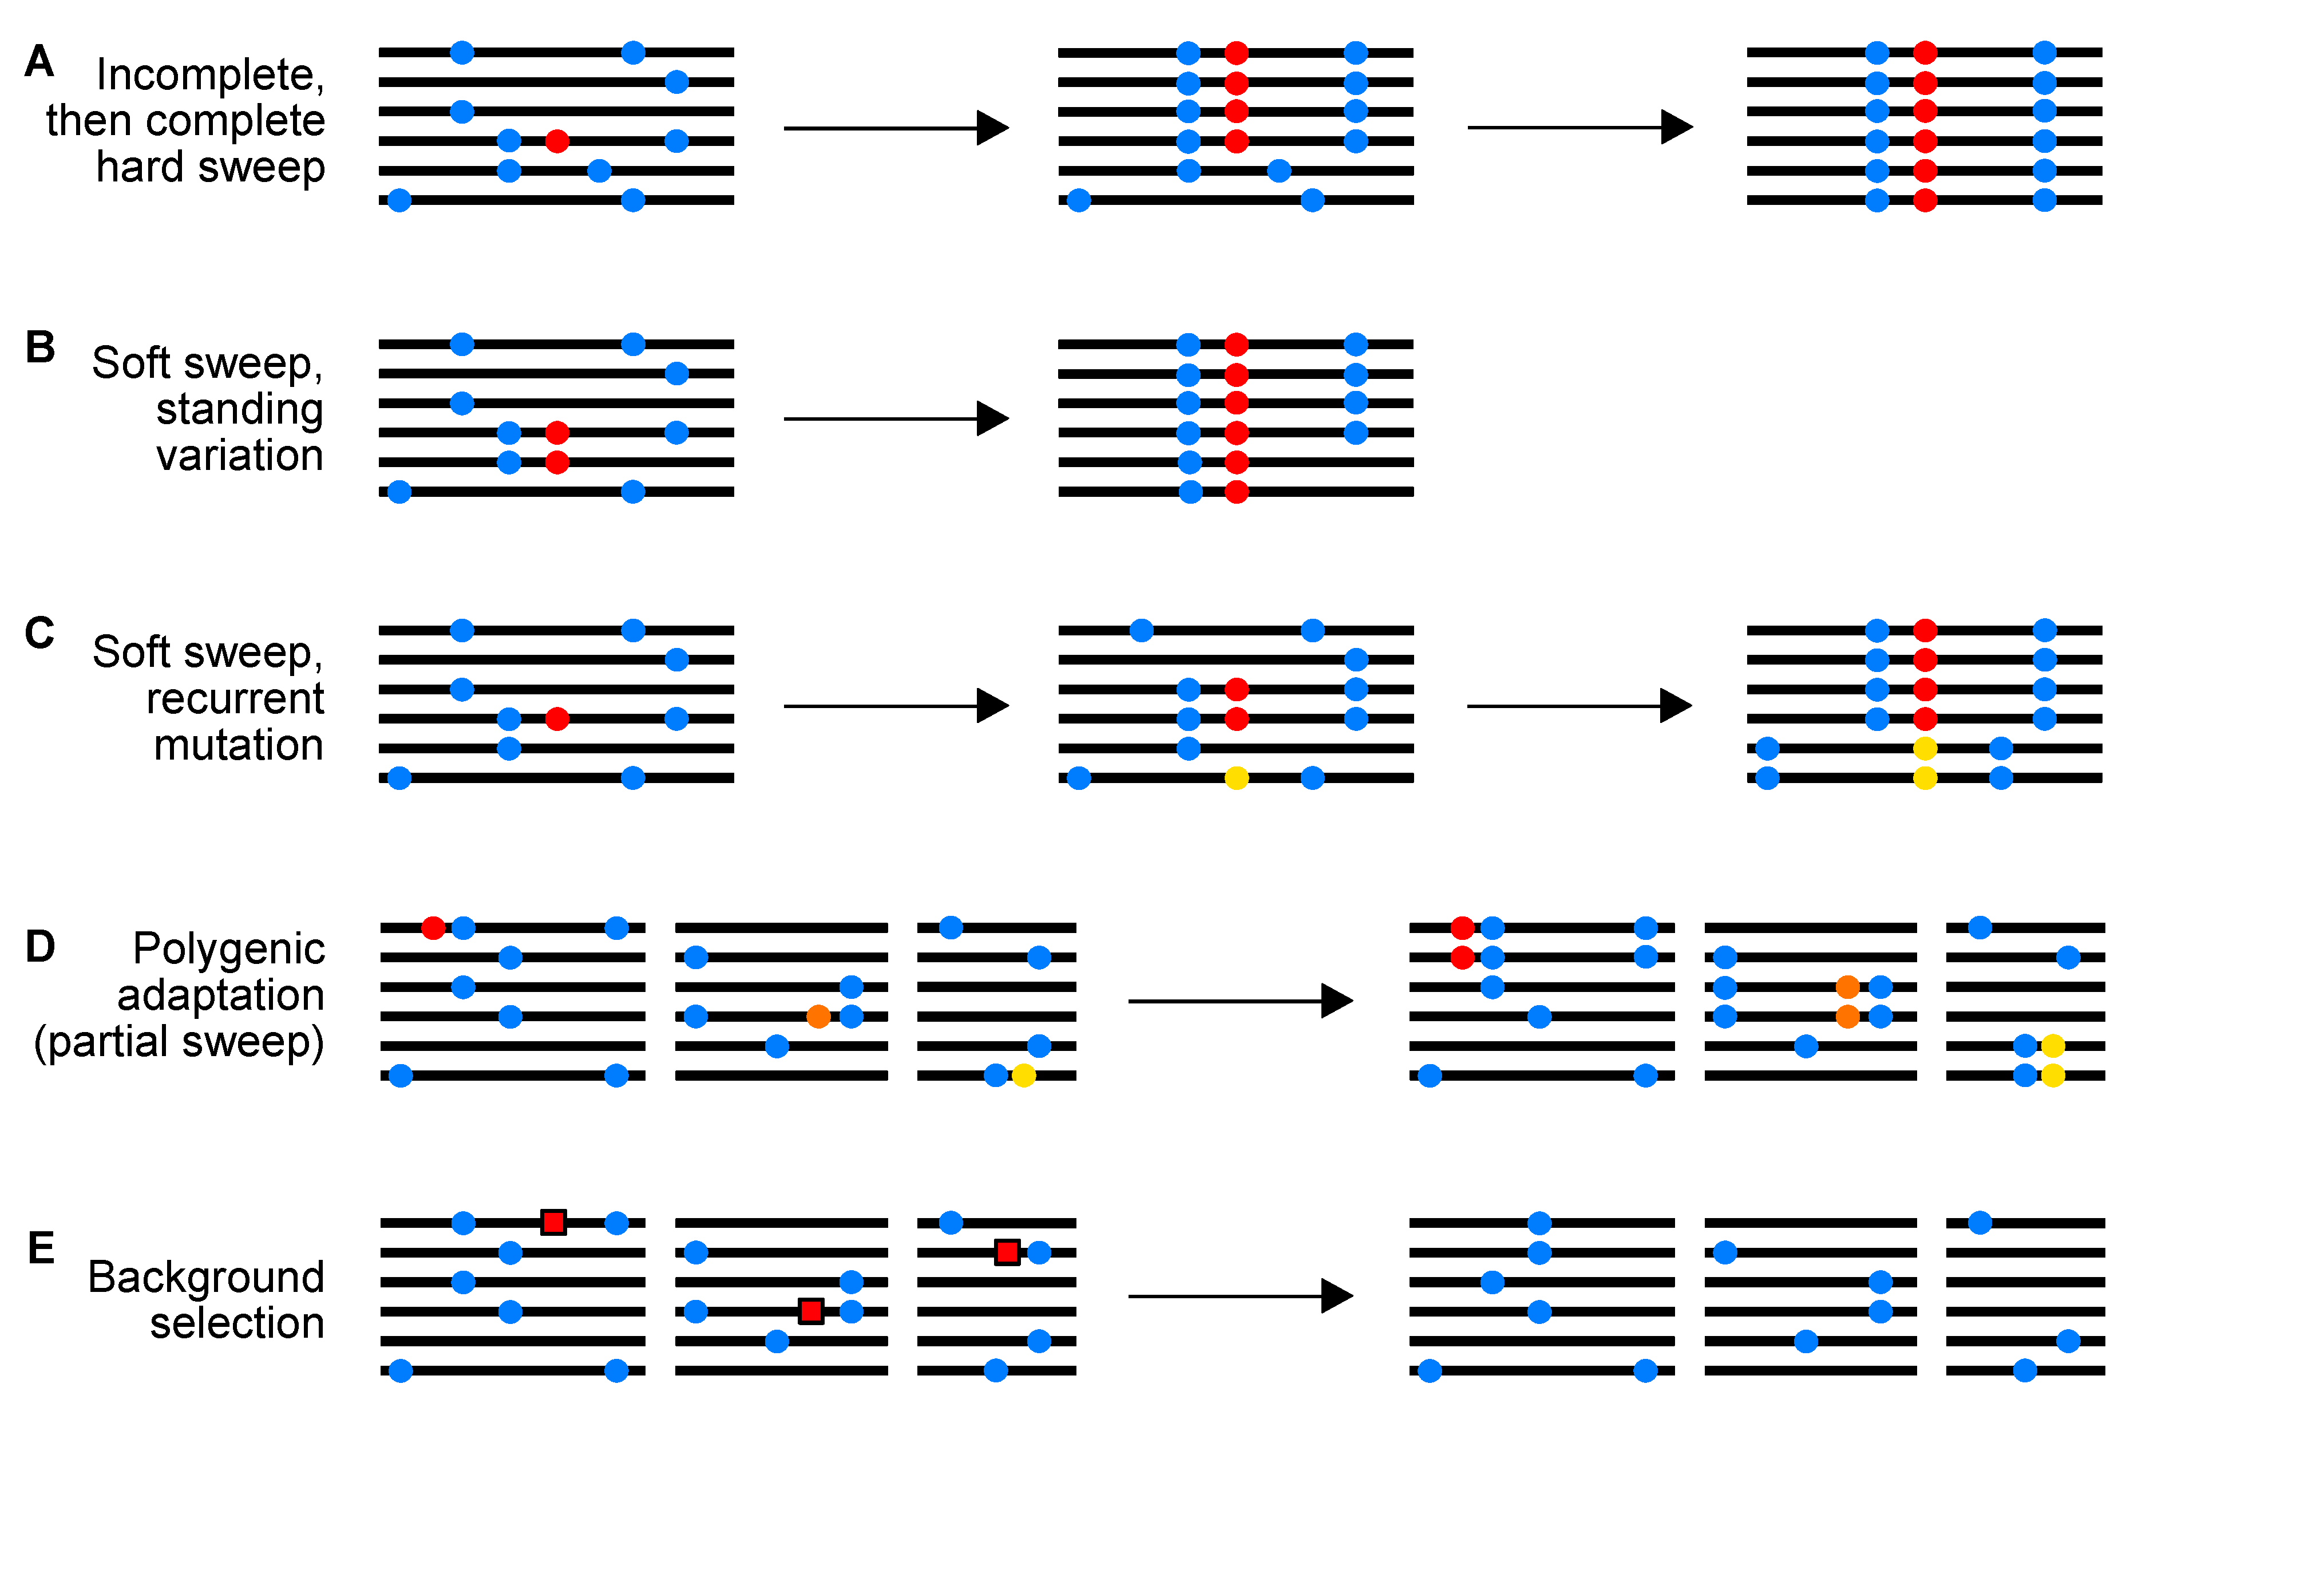
\includegraphics[width=\textwidth]{/Users/s0784966/Dropbox/Thesis/chapter1/figure_sweeps_no_legend.pdf}}
 \caption[Selective sweeps and background selection]{Selective sweeps and background selection. Blue circles represent neutral alleles, red, yellow and orange circles represent advantageous alleles, and red squares represent deleterious alleles. Reproduced from \cite{RN352}, courtesy of Ben Jackson.}.
 
 \label{fig:sweepCartoon}
\end{figure}


\subsubsection{Hard/classic sweeps} 
 
The most well-studied model of sweeps. A new advantageous mutation rapidly increases in frequency to eventual fixation (shown in Figure \ref{fig:sweepCartoon}-A). As it sweeps, the adaptive allele carries with it a portion of the haplotype on which it arose, reducing levels of neutral diversity in the surrounding area \citep{RN124,RN235}. 
 
\subsubsection{Soft sweeps} 
  
A neutral allele segregating in a population may become favoured (due, for example, to a change in the environment). The segregating allele may be associated with multiple haplotypes, and as it rises in frequency, so do the multiple haplotypes (shown in \ref{fig:sweepCartoon}-B). A similar process, also termed a soft sweep, can occur if an advantageous mutation arises by multiple, distinct mutation events (shown in \ref{fig:sweepCartoon}-C). 
 
\subsubsection{Incomplete/partial sweeps} 
 
If an advantageous allele increases in frequency, but does not reach fixation, there will still be some loss of linked neutral diversity. In this review we use the term incomplete sweeps to describe sweeps that are polymorphic at the time of sampling, but may (or may not) eventually reach fixation (shown in \ref{fig:sweepCartoon}-A). The term partial sweep describes the situation wherein a sweeping allele becomes effectively neutral at a certain frequency in its trajectory (shown in \ref{fig:sweepCartoon}-D). The magnitude of both processes on linked neutral diversity depend on the frequency reached by the sweeping allele when selection is ‘turned off’ or on the time of sampling \citep{RN226}. Partial sweeps may be common in cases of adaptation involving selection on quantitative traits \citep{RN147}. 

\subsection{Background selection} 
As natural selection purges deleterious mutations, neutral alleles linked to the selected locus are also lost. The process of background selection is qualitatively similar to recurrent selective sweeps, since both processes reduce local genetic diversity \citep{RN110} and skew the site frequency spectrum towards rare variants \citep{RN287, RN113}. Models of background selection envisage a neutral site linked to many functional sites at different distances, such that the effects of selection at many sites accumulate to reduce diversity \citep{RN206,RN157}. 

\section[Using models of selective sweeps to estimate positive selection parameters]{Using models of selective sweeps to estimate positive selection parameters}
 
Population geneticists have long sought to understand the contribution of natural selection to molecular evolution. A variety of approaches have been proposed that use population genetic theory to quantify the rate and strength of positive selection acting in a species’ genome. In the following section, I discuss methods that use patterns of between-species nucleotide divergence and within-species diversity to estimate positive selection parameters from population genomic data. We also discuss recently proposed methods to detect positive selection from a population’s haplotype structure. The application of these tests has resulted in the detection of pervasive adaptive molecular evolution in multiple species.
 
If adaptive substitutions are common, selection is expected to leave footprints in genetic diversity at linked sites. In particular, as a positively selected mutation increases in frequency, it tends to reduce diversity at linked neutral loci. Theoretical analysis of this process, termed a selective sweep (\textit{see above}), has shown that the reduction in diversity at a linked neutral locus depends on the ratio of the strength of positive selection to the recombination rate. Thus, comparing diversity at multiple neutral loci linked to selected regions, in principle, should provide an indirect means for estimating parameters of positive selection.

If a population experiences recurrent selective sweeps, there are several patterns predicted by theory. Under recurrent hard selective sweeps, levels of genetic diversity are expected to be lower i) in regions of the genome with restricted recombination, ii) in regions experiencing many sweeps and iii) in the genomic regions surrounding the targets of selection themselves. Each of these of these predictions have been met in empirical studies, and each has been used to estimate parameters of positive selection.

\subsection[The correlation between diversity and the rate of recombination]{The correlation between diversity and the rate of recombination}

In the late 1980s, evidence began to emerge suggesting that genetic polymorphism are less frequent in genomic regions experiencing restricted crossing-over \citep{RN225,RN282}. Soon after, \cite{RN114} showed that there is a positive correlation between nucleotide diversity and the rate of crossing-over in \emph{D. melanogaster}, a pattern subsequently observed in other eukaryotic species \citep{RN117}. Begun and Aquadro pointed out that the correlation is qualitatively consistent with the action of recurrent selective sweeps. \cite{RN277} formulated expressions, based on the correlation between nucleotide diversity and the rate of recombination, to estimate the compound parameter $\lambda 2N_{e}s$, where $\lambda$ is the rate of sweeps per base pair per generation, $N_e$ is the effective population size and $s$ is the selection coefficient. They applied their method to the data of \cite{RN114}, estimating $\lambda2N_{e}s$ = 5.37 x $10^{-8}$, but their method could not disentangle the individual parameters. More recently, \cite{RN226} performed a similar analysis in \emph{D. melanogaster} to explore the effects of partial sweeps on parameter estimates. They showed that when partial sweeps are common, the rate of adaptive evolution is underestimated if the hard sweep model is assumed.
 
The correlation between diversity recombination observed by \cite{RN114} can also be explained by background selection, the reduction in neutral diversity caused by the removal of linked deleterious mutations \citep{RN132}. The process of background selection is qualitatively similar to recurrent selective sweeps, since both processes reduce local genetic diversity \citep{RN110} and skew the SFS towards rare variants \citep{RN287,RN133}. Models of background selection envisage a neutral site linked to many functional sites at different distances, such that the effects of selection accumulate to reduce diversity \citep{RN206, RN157}. The correlation between neutral diversity and the recombination rate predicted by background selection is quantitatively similar to that observed in \emph{D. melanogaster} \citep{RN281}. Indeed, recent studies suggest that background selection is a major determinant of nucleotide diversity variation at broad scales ($>$100Kbp) in humans \cite{RN120} and \emph{D. melanogaster} \citep{RN288, RN116}. It is clear, then, that background selection is a key confounding factor when attempting to make inferences about positive selection.
 
\subsection[Correlations between neutral diversity and non-neutral divergence]{Correlation between neutral diversity and non-neutral divergence}

If there is a constant fraction of adaptive substitutions, $\alpha$, across the genome for a given class of sites, regions that evolve at higher rates should experience a greater number of selective sweeps. Under a model of recurrent sweeps, it follows that there should be a negative correlation between nucleotide divergence at selected sites and diversity at linked neutral sites. This was first described in \textit{Drosophila melanogaster} by \cite{RN283}, and has been subsequently reported in other \textit{Drosophila} species \citep{RN284}. Assuming a single rate of sweeps ($\lambda$) and a constant scaled strength of positive selection ($2N_es$) for a given class of sites, \cite{RN283} generalised formulae of \cite{RN277} based on the correlation between synonymous site diversity and non-synonymous site divergence to estimate  $\lambda 2N_es$ = $3 \times 10^{-8}$ for the X-chromosome in \textit{D. melanogaster}. Note that this $\lambda 2N_es$ estimate is similar to that obtained based on the correlation of synonymous site diversity and recombination rate (\cite*{RN277}; see above). Using an estimate of $\alpha = 0.50$ obtained from a MK-based analysis, \cite{RN283} decomposed the $\lambda 2N_es$ compound parameter, and inferred that $s \approx 0.001\%$ and $\lambda$ = $3.6 x 10^{-11}$ /bp/generation, suggesting that adaptation of protein-coding genes in \textit{D. melanogaster} is driven by moderately weak selection (i.e., assuming \textit{D. melanogaster} $N_e =10^6$, $2N_es \approx 40$). In a related study, \cite{RN289} estimated $\lambda 2N_es \approx 10^{-7}$ in \textit{D. simulans}, also by examining the correlation between mean neutral diversity and selected (nonsynonymous) divergence. However, their model also included the heterogeneity in levels of diversity, which is related to the rate and strength of sweeps in a different way to the mean, and allowed the individual parameters to be fitted by regression. The estimates of the compound parameter $\lambda 2N_es$ are similar between the two studies, though \cite{RN289} estimated that $s \approx 1\%$ (compared to Andolfatto’s estimate of $s \approx 0.001 \%$) and $\lambda = 3.6 \times 10^{-12}$ /bp/generation. The discrepancies between the studies may be due to differences in biology between the species, or may reflect methodological differences: For example, if the majority of adaptive substitutions are driven by weakly selected sweeps, which will leave a relatively small signal in levels of  polymorphism, the MK-based method may more sensitively detect them, perhaps explaining the higher rate of sweeps inferred by \cite{RN283}. On the other hand, strongly selected sweeps will leave a larger footprint in levels of diversity, so will be more readily detected using the approach of \cite{RN289}, perhaps explaining why they inferred a lower overall rate of sweeps, with higher selection coefficients (for a full description, see \citealt{RN171}). In both cases, inferences based on variation in polymorphism may reflect processes other than the fixation of adaptive alleles that have gone to fixation, such as partial sweeps and background selection, as these will affect patterns of diversity but not necessarily divergence. Related to this, the approach employed by \cite{RN283} has recently been extended by \cite{RN323}, by estimating the correlation between synonymous site diversity and non-synonymous divergence in the presence of both background selection and gene conversion in \textit{D. melanogaster}. They found that ignoring background selection tends to increase and decrease estimates of selection strength and rate, respectively. The parameter values estimated in their study suggest that 0.02\% of new mutations at nonsynonymous sites are strongly selected ($s \approx 0.03\%$, assuming $N_e$ = $10^6$ for \textit{D. melanogaster}).
 
\subsection[Patterns of diversity around the targets of selection]{Patterns of diversity around the targets of selection}
 
An individual hard selective sweep is expected to leave a trough in genetic diversity around the selected site. If a large proportion of amino acid substitutions are adaptive, as suggested by MK-type analyses (see \citealt{RN215}), collating patterns of diversity around all substitutions of a given type should reveal a trough in diversity. Such a pattern is not expected around a “control” class of sites, such as synonymous sites. This test, proposed by \cite{RN167}, was first applied it to \textit{D. simulans}, and the above pattern was found. By fitting a hard sweeps model to the shape of the diversity trough, they estimated α values of  5\% and 13\%, depending on whether one or two classes of beneficial mutational effects were fitted. Note that their estimates of α are substantially lower than those obtained using MK-based methods for \textit{D. melanogaster} \citealt{RN283}. \cite{RN167} suggested that modes of selection other than hard sweeps may help explain to this discrepancy. However, even when modelling two classes of beneficial mutations, they found that amino acid substitutions are driven by strongly adaptive mutations ($s$ $sim0.5\%$ and $s$ $\sim0.01\%$). Their estimates of selection strength are therefore in broad agreement with the estimate of s $sim1\%$ obtained by \cite{RN289}, based on the correlation between synonymous diversity and non-synonymous divergence in \textit{D. simulans}. The \cite{RN167} test, then, suggests that adaptation in protein-coding genes is fairly frequent and driven by strong, hard sweeps.
 
The Sattath test has been applied in a variety of organisms, including humans \citep{RN162}, wild mice \citep{RN122}, \textit{Capsella grandiflora} \citep{RN236} and maize \citep{RN230}. In all but \textit{C. grandiflora}, researchers have found no difference in patterns of diversity around selected and neutral substitutions. These results have been interpreted as evidence that hard sweeps were rare in the recent history of both humans \citep{RN162} and maize \citep{RN230}. However, \cite{RN237} pointed out that the Sattath test will be underpowered if there is large variation in levels of functional constraint in the genome. Indeed, through their analyses \cite{RN237} found evidence for frequent adaptive substitutions in humans, particularly in regulatory sequence. To address the issues raised by \cite{RN237}, \cite{RN230} applied the Sattath test to substitutions in maize genes with the highest and lowest levels of functional constraint separately, but still found no difference in diversity pattern, suggesting either that hard sweeps have been rare in that species or that there is another confounding factor.
 
One possible explanation is that the species in which the Sattath test did/did not detect hard sweeps have distinct patterns of linkage disequilibrium (LD). LD decays to background levels within hundreds of base-pairs in \textit{D. simulans} \citep{RN283} and \textit{C. grandiflora} \citep{RN271}, whereas in humans, maize and wild mice it decays over distances closer to 10,000bp \citep{RN273,RN327, RN272}. It may be, then, that the Sattath test is only applicable when there is relatively short-range LD, such that the patterns of diversity around selected substitutions do not substantially overlap with the analysis windows around neutral ones. If this were the case, interpreting the similarity in troughs of diversity around selected and neutral substitutions as evidence for a paucity of hard selective sweeps may not be justified in organisms where LD decays over distances of a similar order of magnitude as the width of the diversity troughs themselves.
   	        	  
\section[Fitting genome wide patterns]{Fitting genome wide patterns}

	Methods to estimate the rate and strength of positive selection in the genome employ various combinations of nucleotide diversity, divergence, recombination rates and estimates of background selection effects as summary statistics, averaged over many regions of the genome. Recently, \cite{RN274} developed a method that fits a model of hard sweeps and background selection to genome-wide variation in nucleotide diversity and divergence (at both selected and neutral sites). In \textit{D. melanogaster}, they showed that hard sweeps can explain a large amount of genome-wide variation genetic diversity. For nonsynonymous sites, they found that $\alpha = 4.1\%$ for strongly selected mutations ($s \geq 0.03\%$) and $\alpha = 36.3\%$ for weakly selected mutations ($s \approx 0.0003\%$), summing to $\alpha = 40.4\%$, which is similar to the estimate obtained using the MK-test \citep{RN283}. Their results suggest that accounting for weakly selected mutations may help reconcile the discrepancy between MK-based estimates of the rate and strength of selection and parameters estimated from sweep model predictions, described above.

\cite{RN274} showed that a map of the effects of hard sweeps and background selection is capable of explaining a large amount of the variation in diversity across the genome, further demonstrating that the action of natural selection is pervasive, at least in \textit{D. melanogaster}. However, their method overestimated the rate of deleterious mutations, which the authors attribute to the presence of modes of adaptation other than hard sweeps in \textit{D. melanogaster}. 

\section[\cite{RN122}]{\cite{RN122}}


	The research I have performed throughout my PhD carries on from the work of \cite{RN122}, it is fitting, therefore, to give a brief description of the key findings from that study.
	
	\cite{RN122} sequenced the genomes of 10 wild-caught \textit{Mus musculus castaneus} individuals, using high-throughput sequencing methods. They sequenced individuals to high coverage, using multiple libraries of Illumina paired-end reads. Based on an analysis of population structure, the individuals sequenced were thought to represent a single admixed group. \cite{RN122} extracted polymorphism data from genomic regions surrounding both protein-coding exons and conserved non-coding elements (CNEs - which were inferred to be involved in gene regulation), and found dips (or troughs) in average diversity surrounding the elements themselves. As discussed above, \cite{RN122} applied the Sattath analysis to their data, but found that there was no difference in the average diversity around nonsynonymous/synonymous substitutions. They also modelled the contribution BGS made to the troughs in diversity around both protein-coding exons and CNEs using a population genetic model, and found that it could not fully explain the observed patterns of diversity. Our understanding of the factors that shape nucleotide diversity across the mouse genome are, thus, somewhat unclear.

\section[Thesis aims]{Thesis aims}

	The aim of this thesis is to further our understanding of the factors that shape variation in genetic diversity across the mammalian genome using the house mouse as a model. Particularly, I focus on the contributions of background selection and selective sweeps to variation in genetic diversity across the mouse genome. 

	\begin{itemize}
	
	\item In Chapter 2, I leverage information from patterns of linkage disequilibrium across the mouse genome to construct recombination rate maps for the mouse genome. I use these to investigate the relationship between nucleotide diversity and recombination rate. 
	
	\item In Chapter 3, I estimate the distribution of fitness effects both advantageous and deleterious mutations for multiple classes of sites in the mouse genome. I use these estimates to parametrise forward-in-time population genetic simulations. By analysing these simulations, I attempt to dissect the contributions of selective sweeps and background selection to troughs in diversity around functional elements.
	
	\item In Chapter 4, I fit a model incorporating the effects of selective sweeps and background selection to troughs in diversity around functional elements in mice. Using the parameters that provide the best fit to the data, I ask whether adaptation in protein-coding or  regulatory regions contributes most to fitness change in mice.
	
	\end{itemize}


	% Boot up the Chapter 2: Recombination file
	\chapter{The recombination landscape in wild house mice inferred using population genomic data}
\chaptermark{Recombination in wild mice}

\externaldocument{/Users/s0784966/Dropbox/Thesis/chapter2Appendix/chapter2appendix.tex}

\section{Abstract}
 
Characterizing variation in the rate of recombination across the genome is important for understanding several evolutionary processes. Previous analysis of the recombination landscape in laboratory mice has revealed that the different subspecies have different suites of recombination hotspots. It is unknown, however, whether hotspots identified in laboratory strains reflect the hotspot diversity of natural populations or whether broad-scale variation in the rate of recombination is conserved between subspecies. In this study, we constructed fine-scale recombination rate maps for a natural population of the Eastern house mouse, \textit{Mus musculus castaneus}. We performed simulations to assess the accuracy of recombination rate inference in the presence of phase errors, and we used a novel approach to quantify phase error. The spatial distribution of recombination events is strongly positively correlated between our \textit{castaneus} map and a map constructed using inbred lines derived predominantly from \textit{M. m. domesticus}. Recombination hotspots in wild \textit{castaneus} show little overlap, however, with the locations of double-strand breaks in wild-derived house mouse strains. Finally, we also find that genetic diversity in \textit{\textit{M. m. castaneus}} is positively correlated with the rate of recombination, consistent with pervasive natural selection operating in the genome. Our study suggests that recombination rate variation is conserved at broad scales between house mouse subspecies, but it is not strongly conserved at fine scales.

\section{Introduction}
 
In many species, crossing-over events are not uniformly distributed across chromosomes. Understanding this variation and its causes is important for many aspects of molecular evolution. Experiments in laboratory strains or managed populations that examine the inheritance of markers through pedigrees have produced direct estimates of crossing-over rates in different genomic regions. Studies of this kind are impractical for many wild populations, however, because pedigrees are largely unknown (but see \citealt{RN250}). In mice, there have been several genetic maps published (e.g., \citealt{RN183,RN263,RN232,RN266}), typically using the classical inbred laboratory strains, which are predominantly derived from the Western European house mouse subspecies, \textit{Mus musculus domesticus} \citep{RN243}. Recombination rate variation in laboratory strains may not, therefore, reflect rates and patterns in wild mice of other subspecies. In addition, recombination rate modifiers may have become fixed in the process of laboratory strain management. On the other hand, directly estimating recombination rates in wild house mice is not feasible without both a population’s pedigree and many genotyped individuals (but see \citealt{RN267}). 
 
        	Patterns of linkage disequilibrium (LD) in a sample of individuals drawn from a population can be used to infer variation in the rate of recombination across the genome. Coalescent-based methods have been developed to indirectly estimate recombination rates at very fine scales \citep{RN261, RN182, RN257, RN260, RN213}. Recombination rates estimated in this way reflect long term variation in crossing-over in the population’s history, and are averages between the sexes. Methods using LD have been applied to explore variation in recombination rates among mammals and other eukaryotes, and have demonstrated that recombination hotspots are associated with specific genomic features \citep{RN246, RN247, RN258}.

The underlying mechanisms explaining the locations of recombination events have been the focus of much research. In house mice and in most other mammals, the PRDM9 zinc-finger protein binds to specific DNA motifs, resulting in an increased probability of double-strand breaks (DSBs), which can then be resolved by reciprocal crossing-over or gene conversion \citep{RN245, RN256}. Accordingly, it has been shown that recombination hotspots are enriched for PRDM9 binding sites \citep{RN262, RN156}. PRDM9-knockout mice still exhibit hotspots, but in dramatically different genomic regions \citep{RN254}. Variation in PRDM9, specifically in the exon encoding the zinc-finger array, results in different binding motifs \citep{RN269}. \cite{RN246} generated a line of mice in which the exon encoding the portion of the PRDM9 protein specifying the DNA binding motif was replaced with the orthologous human sequence. The recombination hotspots they observed in this ‘humanized’ line of mice were enriched for the human PRDM9 binding motif. 

Great ape species each have different PRDM9 alleles \citep{RN264} and relatively little hotspot sharing \citep{RN214, RN221}. The broad-scale recombination landscapes of the great apes are, however, strongly positively correlated \citep{RN221}, suggesting that hotspots evolve rapidly, but that the overall genetic map changes more slowly. Indeed, broad-scale recombination rates are positively correlated between closely related species pairs with different hotspot locations \citep{RN174}, and between species that share hotspots or lack them altogether \citep{RN258,RN259}.
 
It has been suggested that a population ancestral to the \textit{M. musculus} subspecies complex split into the present-day subspecies around 350,000 years ago \citep{RN315}. In this time, functionally distinct PRDM9 alleles and distinct suites of hotspots evolved in the different subspecies \citep{RN249}. In addition, there is variation in the recombination rate at relatively broad scales across several regions of the genome between members of the \textit{M. musculus} subspecies complex \citep{RN244}, and recombination rates vary between recently diverged \textit{M. m. domesticus} populations \citep{RN267}. \cite{RN156} analysed single nucleotide polymorphism (SNP) data for classical laboratory strains of mice and used an LD-based approach to estimate the sex-averaged recombination landscape for the 19 autosomes. Their genetic map is similar to a genetic map generated using crosses by \cite{RN232}. However, both studies were conducted using inbred lines whose ancestry is largely \textit{M. m. domesticus} \citep{RN243}, so their recombination landscapes may be different from other members of the \textit{M. musculus} subspecies complex.
 
In this study, we constructed genetic maps for the house mouse subspecies \textit{M. m. castaneus}. We used the genome sequences of 10 wild-caught individuals of \textit{M. m. castaneus} from the species’ assumed ancestral range, originally reported by \cite{RN122}. In our analysis, we first phased SNPs and estimated rates of error in phasing. Secondly, we simulated data to assess the power of estimating recombination rates based on only 10 individuals and the extent by which phase errors lead to biased estimates of the rate of recombination. Finally, using an LD-based approach, we inferred a sex-averaged genetic map and compared this to previously published maps for \textit{M. musculus}. We show that broad-scale variation in recombination rates in \textit{M. m. castaneus} is similar to that seen in the classical inbred strains. However, we show that the locations of potential recombination hotspots in \textit{M. m. castaneus} exhibit little overlap with those reported in wild-derived laboratory strains.

\section{Materials and Methods}
 
\subsection{Polymorphism data for \textit{Mus musculus castaneus}}
 
We analysed the genome sequences of 10 wild-caught \textit{M. m. castaneus} individuals \citep{RN122}. Samples were from North-West India, a region that is believed to be within the ancestral range of the house mouse. Mice from this region have the highest genetic diversity among the \textit{M. musculus} subspecies \citep{RN233}. In addition, the individuals sequenced showed little evidence for substantial inbreeding and a population structure analysis suggested that they represent a single population \citep{RN158}. \cite{RN122} sequenced individual genomes to high coverage using multiple libraries of Illumina paired-end reads, and mapped these to the mm9 reference genome using BWA \citep{RN251}. Mean coverage was $>20x$ and the proportion of the genome with >10x coverage was more than 80\% for all individuals sampled \citep{RN122}. Variants were called with the Samtools mpileup function \citep{RN252} using an allele frequency spectrum (AFS) prior. The AFS was obtained by iteratively calling variants until the spectrum converged. After the first iteration, all SNPs at frequencies >0.5 were swapped into the mm9 genome to construct a reference genome for \textit{M. m. castaneus}, which was used for subsequent variant calling (for further details see \citealt{RN122}). The variant call format (VCF) files generated by \cite{RN122} were used in this study. In addition, alignments of \textit{Mus famulus} and \textit{Rattus norvegicus} to the mm9 genome, also generated by \cite{RN122}, were used as outgroups.
 
	For the purpose of estimating recombination rates, variable sites were filtered on the basis of the following conditions. Insertion/deletion polymorphisms were excluded, because the method used to phase variants cannot process these sites. Sites at which more than two alleles segregated and those that failed the Samtools Hardy-Weinberg equilibrium test ($p$ < 0.002) were also excluded. The hypermutability of CpG sites violates the assumption of a single mutation rate. We defined sites as CpG-prone if they were preceded by a C or followed by a G in \textit{M. m. castaneus}, \textit{M. famulus} or \textit{R. norvegicus}. 
 
\subsection{Inferring phase and estimating switch error rates}
 
LDhelmet estimates recombination rates from a sample of phased chromosomes or haplotypes drawn from a population. To infer haplotypes, heterozygous SNPs called in \textit{M. m. castaneus} were phased using read-aware phasing in ShapeIt2 \citep{RN231}, which phases variants at the level of whole chromosomes using sequencing reads that span multiple heterozygous sites (phase-informative reads, PIRs), and LD. Incorrectly phased heterozygous sites, termed switch errors, tend to upwardly bias estimates of the recombination rate, because they appear identical to legitimate crossing-over events. To assess the impact of incorrect phasing on recombination rate inference, we quantified the switch error rate as follows. The sample of \textit{M. m. castaneus} comprised seven females and three males. The X-chromosome variants in males therefore represent perfectly phased haplotypes. We merged the BAM alignments of short reads for the X-chromosomes of the three males (samples H12, H28 and H34 from \citealt{RN122}) to make three datasets of pseudo-females where the true haplotypes are known (H12+H28 = H40; H12+H34 = H46; H28 + H34 = H62). We then jointly re-called variants in the seven female samples plus the three pseudo-females using an identical pipeline as \cite{RN122}, using the same AFS prior.
 
Switch error rates in Shapeit2 are sensitive both to coverage and quality (per genotype and per variant) \citep{RN231}. We explored the effects of different filter parameters on switch error rates using the X-chromosomes of the pseudo-females. We filtered SNPs based on combinations of variant and genotype quality scores (QUAL and GQ, respectively) and on an individual’s sequencing depth (DP) (Table \ref{tab:C2ST1}). For the individual-specific statistics (DP and GQ), if a single individual failed a particular filter, then that SNP was excluded from further analyses. By comparing the known X-chromosome haplotypes and those inferred by ShapeIt2, we calculated switch error rates as the ratio of incorrectly resolved heterozygous SNPs to the total number of heterozygous SNPs for each pseudo-female individual. We used these results to apply filter parameters to the autosomal data that generated a low switch error rate, while maintaining a high number of heterozygous SNPs. We obtained 20 phased haplotypes for each of the 19 mouse autosomes and 14 for the X-chromosome (plus the 3 from the male samples). With these, we estimated the recombination rate landscape for \textit{M. m. castaneus}.
 
\subsection{Estimating genetic maps and validation of the approach}
 
	LDhelmet (v1.7; \citealt{RN213}) generates a sex-averaged genetic map from a sample of haplotypes assumed to be drawn from a randomly mating population. Briefly, LDhelmet examines patterns of LD in a sample of phased chromosomal regions and uses a composite likelihood approach to infer recombination rates between adjacent SNPs. LDhelmet appears to perform well for species of large effective population size ($N_e$) and has been shown to be robust to the effects of selective sweeps, which appear to reduce diversity in and around functional elements of the \textit{M. m. castaneus} genome \citep{RN122}. The analyses of \cite{RN213}, in which the software was tested, were performed with a larger number of haplotypes than we have in our sample. To assess whether our smaller sample size still gives reliable genetic maps, we validated and parameterized LDhelmet using simulated datasets (see below). It should be noted, however, that model underlying LDhelmet assumes recombination-drift equilibrium. Violation of this assumption may therefore result in biased recombination rate estimates. 
 
	A key parameter in LDhelmet is the block penalty, which determines the extent by which likelihood is penalized by spatial variation in the recombination rate, such that a high block penalty results in a smoother recombination map. We performed simulations to determine the block penalty that produces the most accurate estimates of the recombination rate in chromosomes that have diversity and base content similar to \textit{M. m. castaneus}. Chromosomes with constant values of $\rho$ ($4N_er$) ranging from 2 x $10^{-6}$ to 2 x $10^1$ were simulated in SLiM v1.8 \citep{RN148}. For each value of $\rho$, 0.5Mbp of neutrally evolving sequence was simulated for populations of N = 1,000 diploid individuals. Mutation rates in the simulations were set using the compound parameter $\theta$ = $4N_e\mu$, where $\mu$ is the per-base, per-generation mutation rate. The mutation and recombination rates of the simulations were scaled to $\theta /4N$ and $\rho /4N$, respectively. $\theta$ was set to 0.01 in the simulations, because this value is close to the genome-wide average for our data, based on pairwise differences. Simulations were run for 10,000 generations in order to achieve equilibrium diversity, at which time 10 diploid individuals were sampled. Each simulation was repeated 20 times, resulting in 10Mbp of sequence for each value of ρ. The SLiM output files were converted to sequence data suitable for analysis by LDhelmet using a custom Python script that incorporated the mutation rate matrix estimated for non-CpG prone sites in \textit{M. m. castaneus} (see below). Following \cite{RN213}, we inferred recombination rates from the simulated data in windows of 4,400 SNPs with a 200 SNP overlap between windows. We analysed the simulated data using LDhelmet with block penalties of 10, 25, 50 and 100. The default parameters of LDhelmet are tuned to analyze Drosophila melanogaster data \citep{RN213}. Since the \textit{D. melanogaster} population studied by \cite{RN213} has comparable nucleotide diversity to \textit{M. m. castaneus}, we used default values for other parameters, with the exception of the block penalty.
 
	Errors in phase inference, discussed above, may bias our estimates of the recombination rate, since they appear to break apart patterns of LD. We assessed the impact of these errors on recombination rate inference by incorporating them into the simulated data at a rate estimated from the pseudo-female individuals. For each of the 10 individuals drawn from the simulated populations, switch errors were randomly introduced at heterozygous positions at the rate estimated using the SNP filter set chosen on the basis of the pseudo-female analysis (see Results). We then inferred recombination rates for the simulated population using these error-prone data, as above. We assessed the effect of switch errors on recombination rate inference by comparing estimates from the simulated data with and without switch errors. It is worth noting that switch errors may undo crossing-over events and thereby reduce inferred recombination rates if they affect heterozygous SNPs located at recombination breakpoints.

\subsection{Recombination rate estimation for \textit{\textit{M. m. castaneus}}}
        	
         We used LDhelmet \citep{RN213} to estimate recombination rate landscapes for each of the \textit{M. m. castaneus} autosomes and the X-chromosome. A drawback of LD-based approaches is that they estimate sex-averaged recombination rates. This is a limitation of our study as there are known differences in recombination rates between the sexes in \textit{M. musculus} \citep{RN232,RN266}.
 
        	We used \textit{M. famulus} and \textit{R. norvegicus} as outgroups to assign ancestral states for polymorphic sites. LDhelmet incorporates the mutation matrix and a prior probability on the ancestral allele at each variable position as parameters in the model. We obtained these parameters as follows. For non-CpG prone polymorphic sites, if the two outgroups shared the same allele, we assigned that allele as ancestral, and such sites were then used to populate the mutation matrix \citep{RN213}. This approach ignores the possibility of back mutation and homoplasy. To account for this uncertainty, LDhelmet incorporates a prior probability on the ancestral base. Following \cite{RN258}, at resolvable sites (i.e., where both outgroups agreed) the ancestral base was given a prior probability of 0.91, with 0.03 assigned to each of the three remaining bases. This was done to provide high confidence in the ancestral allele, but also to include the possibility of ancestral allele misinference. At unresolved sites (i.e., if the outgroups disagreed or there were alignment gaps in either outgroup), we used the stationary distribution of allele frequencies from the mutation rate matrix as the prior (Table \ref{tab:C2ST2}).
 
We analysed a total of 44,835,801 SNPs in LDhelmet to construct genetic maps for the \textit{M. m. castaneus} autosomes and the X-chromosome. Following \cite{RN213}, windows of 4,400 SNPs, overlapping by 200 SNPs on either side were analysed. We ran LDhelmet for a total of 1,000,000 iterations, discarding the first 100,000 as burn-in. A block penalty of 100 was chosen to obtain conservatively estimated broad-scale genetic maps. For the purposes of identifying recombination hotspots, we re-ran the LDhelmet analysis with a block penalty of 10. We analysed all sites that passed the filters chosen using the pseudo-female phasing analysis regardless of CpG status; note that excluding CpG-prone sites removes ~50\% of the available data and thus would substantially reduce the power to infer recombination rates. We assumed $\theta$ = 0.01, the approximate genome-wide level of neutral diversity in \textit{M. m. castaneus}, and included ancestral allele priors and the mutation rate matrix for non-CpG sites as parameters in the model. Following the analyses, we removed overlapping SNPs and concatenated SNP windows to obtain recombination maps for whole chromosomes. 

It is worthwhile noting that our genetic maps were constructed with genotype calls made using the mm9 version of the mouse reference genome. This version was released in 2007 and there have been subsequent versions released since then. However, previously published genetic maps for \textit{M. musculus} were constructed using mm9, so we used that reference to make comparisons (see below).
 
\subsection{Broad-scale comparison to previously published maps}
 
We compared the \textit{M. m. castaneus} genetic map inferred using a block penalty of 100 with two previously published maps for \textit{M. musculus}. The first map was generated by analyzing the inheritance patterns of markers in crosses between inbred lines \citep{RN232} (downloaded from http://cgd.jax.org/mousemapconverter/). We refer to this map as the Cox map. The second map was generated by \cite{RN146} by analyzing SNPs in classical inbred mouse lines using LDhat \citep{RN260}, the software upon which LDhelmet is based (available at http://www.genetics.org/content/early/2012/05/04/genetics.112.141036). We refer to this map as the Brunschwig map. The Cox and Brunschwig maps were constructed using far fewer markers than the present study, i.e., ~500,000 and ~10,000 SNPs, respectively, compared to the ~45,000,000 used to generate ours. Recombination rate variation in the Cox and Brunschwig maps likely reflects that of \textit{M. m. domesticus}, since both were generated using classical strains of laboratory mice, which are predominantly of \textit{M. m. domesticus} origin \citep{RN243}. For example, in the classical inbred strains analysed by \cite{RN213}, the mean genome-wide ancestry attributable to \textit{M. m. domesticus}, \textit{M. m. musculus} and \textit{M. m. castaneus} are 94.8\%, 5.0\% and 0.2\%, respectively (data downloaded from the Mouse Phylogeny Viewer \citep{RN280} http://msub.csbio.unc.edu). The ancestry proportions for all classical strains, 60 of which were analysed by \cite{RN156}, are similar \citep{RN243}.

Recombination rates in the Brunschwig map and our \textit{castaneus} map were estimated in units of $\rho$ = $4N_er$. For comparison purposes, we converted these units to cM/Mb using frequency-weighted means, as follows. LDhat and LDhelmet provide estimates of $\rho$ (per Kbp and bp, respectively) between pairs of adjacent SNPs. For each chromosome, we calculated cumulative $\rho$, while accounting for differences in the physical distance between adjacent SNPs by using the number of bases separating a pair of SNPs to weight that pair’s contribution to the total. By setting the total map length for each chromosome to that of \cite{RN232}, we converted the cumulative $\rho$ at each analysed SNP position to cM values.
 
At the level of whole chromosomes, we compared mean recombination rate estimates for \textit{castaneus} with several previously published maps. Frequency-weighted mean recombination rates (in terms of $\rho$) for each chromosome in the \textit{castaneus} and Brunschwig maps were compared with cM/Mb values obtained by \cite{RN232} and with independent estimates of per chromosome recombination rates \citep{RN184}. Pearson correlations were calculated for each comparison 
 
At the Mbp scale, we compared variation in recombination rates across the autosomes in the different maps using windows of varying length. We calculated Pearson correlations between the frequency weighted-mean recombination rates (in cM/Mb) in non-overlapping windows of 1Mbp to 20Mbp for the castaneus, Cox and Brunschwig maps. For visual comparison of the \textit{castaneus} and Cox maps, we plotted recombination rates in sliding windows of 10Mbp, offset by 1Mb. 

\subsection{Fine-scale recombination rate variation}

To assess the distribution of recombination events in \textit{M. m. castaneus} on a fine scale, we used Gini coefficients and Lorenz curves as quantitative measures of the extent of heterogeneity (e.g., \citealt{RN333}). In the context of a genetic map, Gini coefficients close to zero represent more uniform distributions of crossing-over rates, whereas values closer to one indicate that recombination events are restricted to a small number of locations. We analysed genetic maps generated using a block penalty of 10 to construct Lorenz curves and calculated their Gini coefficients for each chromosome separately.

	Recombination hotspots can be operationally defined as small windows of the genome that exhibit elevated rates of recombination relative to surrounding regions. To estimate the locations of potential recombination hotspots, we adapted a script used by \cite{RN258}. We divided the genome into non-overlapping windows of 2Kbp, and, using the maps generated with a block penalty of 10, classified as putative hotspots all windows where the recombination rate was at least 5x greater than the recombination rate in the surrounding 80Kbp. Recombination hotspots may be wider than 2Kbp, so neighbouring analysis windows that exhibited elevated recombination rates were merged.

	We investigated whether fine-scale recombination rate variation in wild-caught \textit{M. m. castaneus} is similar to that reported for wild-derived inbred lines. \cite{RN249} generated sequencing reads corresponding to the locations of DSBs (hereafter DSB hotspots) in inbred strains of mice derived from each of the principal \textit{M. musculus} subspecies and \textit{M. m. molossinus}, an inter-sub-specific hybrid of \textit{M. m. castaneus} and \textit{M. m. musculus}. We used the overlap between our putative hotspots and their DSB hotspots for testing similarity. However, the coordinates of DSB hotspots were reported with respect to the mm10 genome \citep{RN249}. To allow comparisons with our putative hotspots, we converted the coordinates of DSB breaks in the mm10 reference to mm9 coordinates using the UCSC LiftOver tool (https://genome.ucsc.edu/cgi-bin/hgLiftOver), with default parameters. We compared the locations of putative hotspots identified in our \textit{castaneus} map with the locations of DSB hotspots using BedTools v2.17.0 \citep{RN279} by counting the number that overlapped. To determine the number of overlaps expected to be seen by chance, we used a randomization approach as follows. The locations of our putative hotspots were randomized with respect to chromosome, and these shuffled coordinates were compared to the locations of DSB hotspots. For each of the inbred strains analysed by \cite{RN249} this procedure was repeated 1,000 times. The maximum number of overlapping DSB and putative \textit{castaneus} hotspots observed across all 1,000 replicates was taken as an approximate 0.1\% significance threshold.
 
\subsection{Examining the correlation between recombination rate and properties of protein coding genes}

We used our \textit{castaneus} map to examine the relationship between recombination rates and nucleotide diversity and divergence as follows. We obtained the coordinates of the canonical spliceforms of protein coding genes, orthologous between mouse and rat from Ensembl Biomart (Ensembl Database 67; http://www.ensembl.org/info/website/ archives/index.html). For each protein coding gene, we calculated the frequency-weighted mean recombination rate from the broad-scale map. Using the approximate \textit{castaneus} reference described above, along with the outgroup alignments, we obtained the locations of 4-fold degenerate synonymous sites and current GC content for each gene. If a site was annotated as 4-fold in all three species considered, it was used for further analysis. We removed poor quality alignments between mouse and rat that exhibited spurious excesses of mismatched sites, where >80\% of sites were missing. We also excluded five genes where there were mismatches with the rat sequence at all non-CpG prone 4-fold sites, since it is likely that these also represent incorrect alignments. After filtering, there were a total of 18,171 protein-coding genes for analysis.

We examined the correlation between the local recombination rate in protein-coding genes and nucleotide diversity, divergence from the rat and GC-content. Variation in the mutation rate across the genome is a potentially important confounding factor. For example, if the recombination rate and mutation rate are positively correlated, we would expect a positive correlation between neutral nucleotide diversity and recombination rate. Because of this, we also examined the correlation between the ratio of nucleotide diversity to divergence from \textit{R. norvegicus} at putatively neutral sites and the rate of recombination. We calculated correlations for all sites and for non-CpG-prone sites only. We used non-parametric Kendall rank correlations for all comparisons.

Analyses were conducted using Python scripts, except for the correlation analyses, which were conducted using R (R Core Team 2016) and hotspot identification, which was done using a Python script adapted from one provided by \cite{RN258}. 

\subsection{Data availability}

	The authors confirm that all data necessary for performing the analyses described in the article are fully described in the text. Recombination maps are available in a compressed form from \textit{https://github.com/TBooker/M.m.castaneus\textunderscore recombination-maps}.

\section{Results}
 
\subsection{SNP phasing and estimating the switch error rate}
 
To infer genetic maps using our sample of individuals, we required phased SNPs. Taking advantage of the high sequencing depth of the sample generated by \cite{RN122}, and using a total of 44,835,801 SNPs (Table \ref{tab:C2ST3}), we phased SNPs using ShapeIt2, an approach that uses LD and sequencing reads to resolve haplotypes. 
 
We quantified the switch error rate incurred when inferring phase by analyzing pseudo-female individuals. After filtering variants, ShapeIt2 returned low switch error rates for all parameter combinations tested (Table \ref{tab:C2ST1}). We therefore applied a set of filters (GQ > 15, QUAL > 30) to apply to the actual data that predicted a mean switch error rate of 0.46\% (Table \ref{tab:C2ST1}). When applied to the actual data these filters removed 44\% of the total number of called SNPs (Table \ref{tab:C2ST3}). More stringent filtering resulted in slightly lower mean switch error rates, but also removed many more variants (Table \ref{tab:C2ST1}), reducing our ability to estimate recombination rates at a fine scale.
 
\subsection{Simulations to validate the application of LDhelmet}

We used simulations to assess the performance of LDhelmet when applied to our dataset. In the absence of switch errors, LDhelmet accurately inferred the average recombination rate down to values of $\rho bp^{-1}$ = 2 x $10^{-4}$. Below this value, LDhelmet overestimated the scaled recombination rate (Figure \ref{fig:C2F1}). With switch errors incorporated into simulated data, LDhelmet accurately estimated $\rho /bp$ in the range 2 x $10^{-3}$ to 2 x $10^2$. When the true $\rho bp^{-1}$ was $<$ 2 x $106{-3}$, however, LDhelmet overestimated the mean recombination rate for 0.5Mbp regions (Figure \ref{fig:C2F1}). This behavior was consistent for all block penalties tested (Figure \ref{fig:C2SF1}). We found that inferred rates of recombination typically fell within the range accurately estimated by LDhelmet (Table \ref{tab:C2T1}; Figure \ref{fig:C2SF2}).
 
  \begin{figure}[h]
   \centering      
   \noindent\makebox[\textwidth]{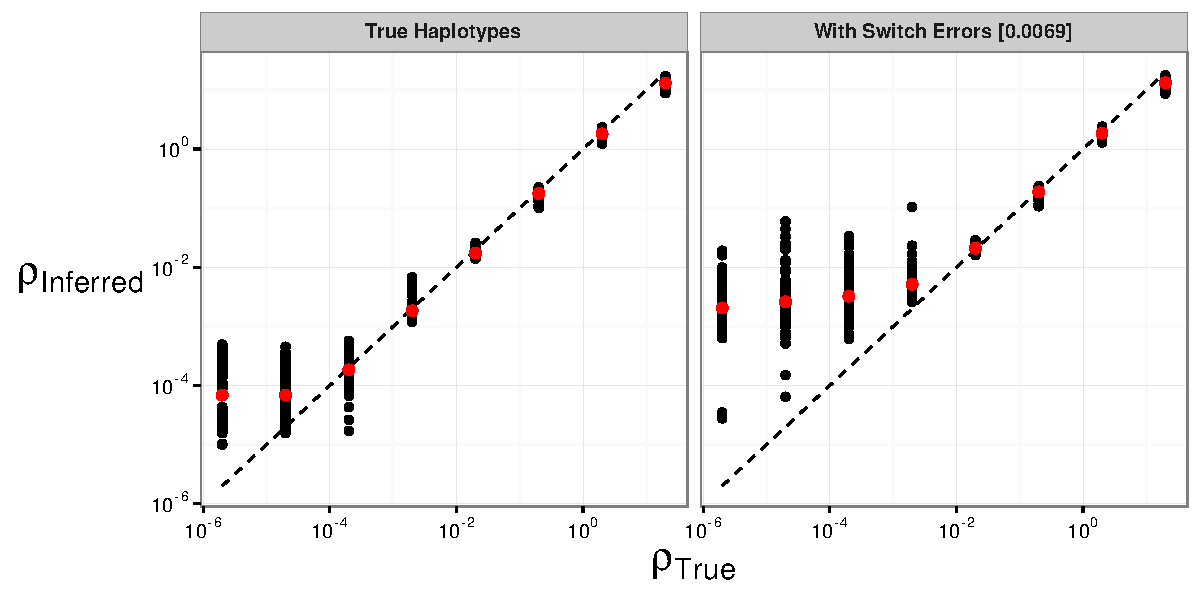
\includegraphics[width=\textwidth]{/Users/s0784966/Dropbox/Thesis/chapter2/Figures/Figure1.pdf}}
 \caption[The effect of switch errors on recombination rate inference]{The effect of switch errors on the mean recombination rate inferred using LDhelmet with a block penalty of 100. Each black point represents results for a window of 4000 SNPs, with 200 SNPs overlapping between adjacent windows, using sequences simulated in SLiM for a constant value of $\rho/bp$. Red points are mean values. Switch errors were randomly incorporated at heterozygous SNPs with probability 0.0046. The dotted line shows the value when the inferred and true rates are equal}
\label{fig:C2F1}
\end{figure}

\subsection{Recombination rates in the \textit{\textit{M. m. castaneus}} genome}
 
We constructed two maps of recombination rate variation for \textit{M. m. castaneus} using LDhelmet. The first was a broad-scale map constructed using a block penalty of 100 (hereafter referred to as the broad-scale map). For the second fine-scale map, we used a block penalty of 10 (hereafter referred to as the fine-scale map). A comparison of broad and fine-scale maps for a representative region of the genome is shown in Figure \ref{fig:C2SF2}. We analysed a total of 44,835,801 phased SNPs across the 19 mouse autosomes and the X-chromosome. From the broad-scale map, the frequency-weighted mean estimate of $\rho /bp$ for the autosomes was 0.0092. This value is higher than the lower detection limit suggested by the simulations with and without switch errors (Figure \ref{fig:C2F1}). For the X-chromosome, the frequency-weighted mean $\rho /bp$ was 0.0026, which is still above the lower detection limit (Figure \ref{fig:C2F1}). The lower SNP density on the X-chromosome (Table \ref{tab:C2ST3}) and the smaller number of alleles available (17 compared to 20 used for the autosomes) may reduce precision. 
 
We assessed variation in whole-chromosome recombination rates between our LD-based \textit{castaneus} map and direct estimates of recombination rates published in earlier studies. Comparing the mean recombination rates of whole chromosomes provides us with a baseline for which we have two a priori expectations. Firstly, we expect that chromosome 19, the shortest in physical length, should have the highest mean recombination rate, since at least one crossing-over event is required per meiosis per chromosome. Secondly, we expect that the X-chromosome, which only undergoes recombination in females, should have the lowest rate. These expectations are borne out in the results (Table \ref{tab:C2T1}), and are consistent with previous studies \citep{RN184, RN232}. We also found that frequency-weighted chromosomal recombination rates (inferred in terms of $\rho = 4N_er$) were highly correlated with the direct estimates (in cM/Mbp) from \cite{RN184} (Pearson correlation coefficient = 0.59, $p$ = 0.005) and \cite{RN232} (Pearson correlation coefficient = 0.68, $p$ = 0.001). Excluding the X-chromosomes does not substantially change these correlations. These results therefore suggest that our analysis captures real variation in the rate of recombination on the scale of whole chromosomes. 


\begin{figure}[h]
   \centering      
   \noindent\makebox[\textwidth]{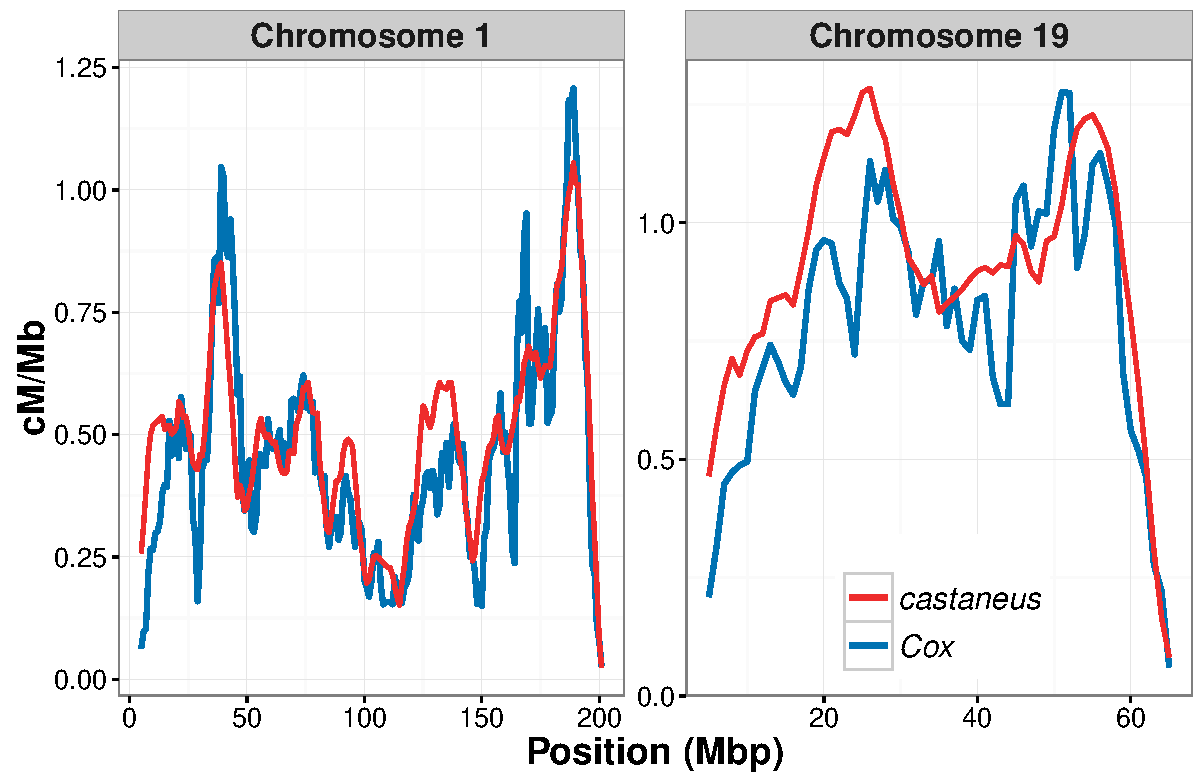
\includegraphics[width=\textwidth]{/Users/s0784966/Dropbox/Thesis/chapter2/Figures/Figure2.pdf}}
 \caption[Comparison of LD-based and pedigree-based recombination maps]{Comparison of sex-averaged recombination rates for chromosomes 1 and 19 of \emph{M. m. castaneus} inferred by LDhelmet (red) with rates estimated in the pedigree-based study of \cite{RN232} (blue). Recombination rates were scaled to units of centimorgans per megabase for the \textit{castaneus} map by setting the total map length of each chromosome to the corresponding map length of \cite{RN232}.}
\label{fig:C2F2}

\end{figure}

\linespread{1}

\begin{sidewaystable}
\caption[Summary of recombination rates per chromosomes]{Summary of sex-averaged recombination rates \emph{M. m castaneus} compared with the rates from Brunschwig et al. (2012) and Cox et al. (2009). Rates for the castaneus and Brunschwig maps are presented in terms of $4N_{e}r/bp$. Estimates of $N_e$ were obtained by assuming the recombination rates from Cox et al. (2009).}
 \begin{tabular}{c c c c c c} 
  \hline
 Chromosome & Cox cM/Mb & Freq. Weighted Mean & $N_e$ Estimate & Freq. Weighted Mean & $N_e$ Estimate \\ [0.5ex] 

 \hline
 1 & 0.50 & 0.0079 & 395,000 & 0.000015 & 745\\
 2 & 0.57 & 0.0088 & 386,000 & 0.000015 & 653\\
 3 & 0.52 & 0.0083 & 400,000 & 0.000014 & 693\\
 4 & 0.56 & 0.0091 & 408,000 & 0.000020 & 889\\
 5 & 0.59 & 0.0090 & 382,000 & 0.000015 & 646\\
 6 & 0.53 & 0.0089 & 421,000 & 0.000015 & 728\\
 7 & 0.58 & 0.0100 & 429,000 & 0.000019 & 801\\
 8 & 0.58 & 0.0094 & 404,000 & 0.000014 & 610\\
 9 & 0.61 & 0.0096 & 394,000 & 0.000018 & 749\\
 10 & 0.61 & 0.0096 & 392,000 & 0.000023 & 928\\
 11 & 0.70 & 0.0102 & 365,000 & 0.000019 & 689\\
 12 & 0.53 & 0.0089 & 420,000 & 0.000019 & 897\\
 13 & 0.56 & 0.0095 & 426,000 & 0.000014 & 629\\
 14 & 0.53 & 0.0084 & 395,000 & 0.000013 & 632\\
 15 & 0.56 & 0.0083 & 371,000 & 0.000024 & 1,080\\
 16 & 0.59 & 0.0091 & 386,000 & 0.000017 & 721\\
 17 & 0.65 & 0.0087 & 335,000 & 0.000052 & 2,020\\
 18 & 0.66 & 0.0098 & 371,000 & 0.000021 & 785\\
 19 & 0.94 & 0.0122 & 323,000 & 0.000026 & 681\\
 X & 0.48 & 0.0026 & 137,000 & - & -\\
 Mean & - & 0.0092 & - & 0.000020 &  -\\[1ex] 
 \hline
\end{tabular}    

\end{sidewaystable}


\linespread{2}

\subsection{Comparison of the \textit{M. m. castaneus} map with maps constructed using inbred lines}
 
        	We then compared intra-chromosomal variation in recombination rates between our broad-scale \textit{castaneus} map and previously published maps. Figure \ref{fig:C2F2} shows a comparison of recombination rates inferred from the \textit{castaneus} and Cox maps for the longest and shortest autosomes, chromosomes 1 and 19, respectively. It is clear that the \textit{castaneus} and Cox maps are very similar (see also Figure \ref{fig:C2SF3}). We compared recombination rates in the \textit{castaneus} and Cox maps in genomic intervals of various sizes and found that correlation coefficients were >0.8 for window sizes of 8Mbp and above (Figure \ref{fig:C2F3}). The correlations are smaller if chromosomes are considered separately (Figure \ref{fig:C2SF4}). Although the correlation coefficients are generally high (Figure \ref{fig:C2F3}), there are several regions of the genome where the \textit{castaneus} and Cox maps have substantially different recombination rates, for example in the center of chromosome 9 (Figure \ref{fig:C2SF3}). The Cox and \textit{castaneus} maps are more similar to one another than either are to the Brunschwig map (Figure \ref{fig:C2F3}). This is presumably because the Brunschwig map was constructed with a relatively low SNP density and by an LD-based approach using a sample of inbred mouse strains, which violates key assumptions of the method. Population structure in the lines analysed by \cite{RN156} or the subspecies from which they were derived would elevate LD, resulting in lower chromosome-wide values of $\rho$. The average scaled recombination rate estimates differ substantially between the \textit{castaneus} and Brunschwig maps, i.e., the \textit{castaneus} chromosomal estimates are ~500x higher (Table \ref{tab:C2T1}). This is also reflected in $N_e$, estimated on the basis of the frequency-weighted average recombination rates for each chromosome. Independent polymorphism data suggest that effective populations sizes for \textit{M. m. castaneus} and \textit{M. m. domesticus} are approximately 100,000 and 500,000 respectively \citep{RN255,RN315}. Estimates of $N_e$ from the \textit{castaneus} map are therefore in line with expectation, while those from the Brunschwig map are not (Table \ref{tab:C2T1}).


\linespread{1}
\begin{figure}[h]
   \centering      
   \noindent\makebox[\textwidth]{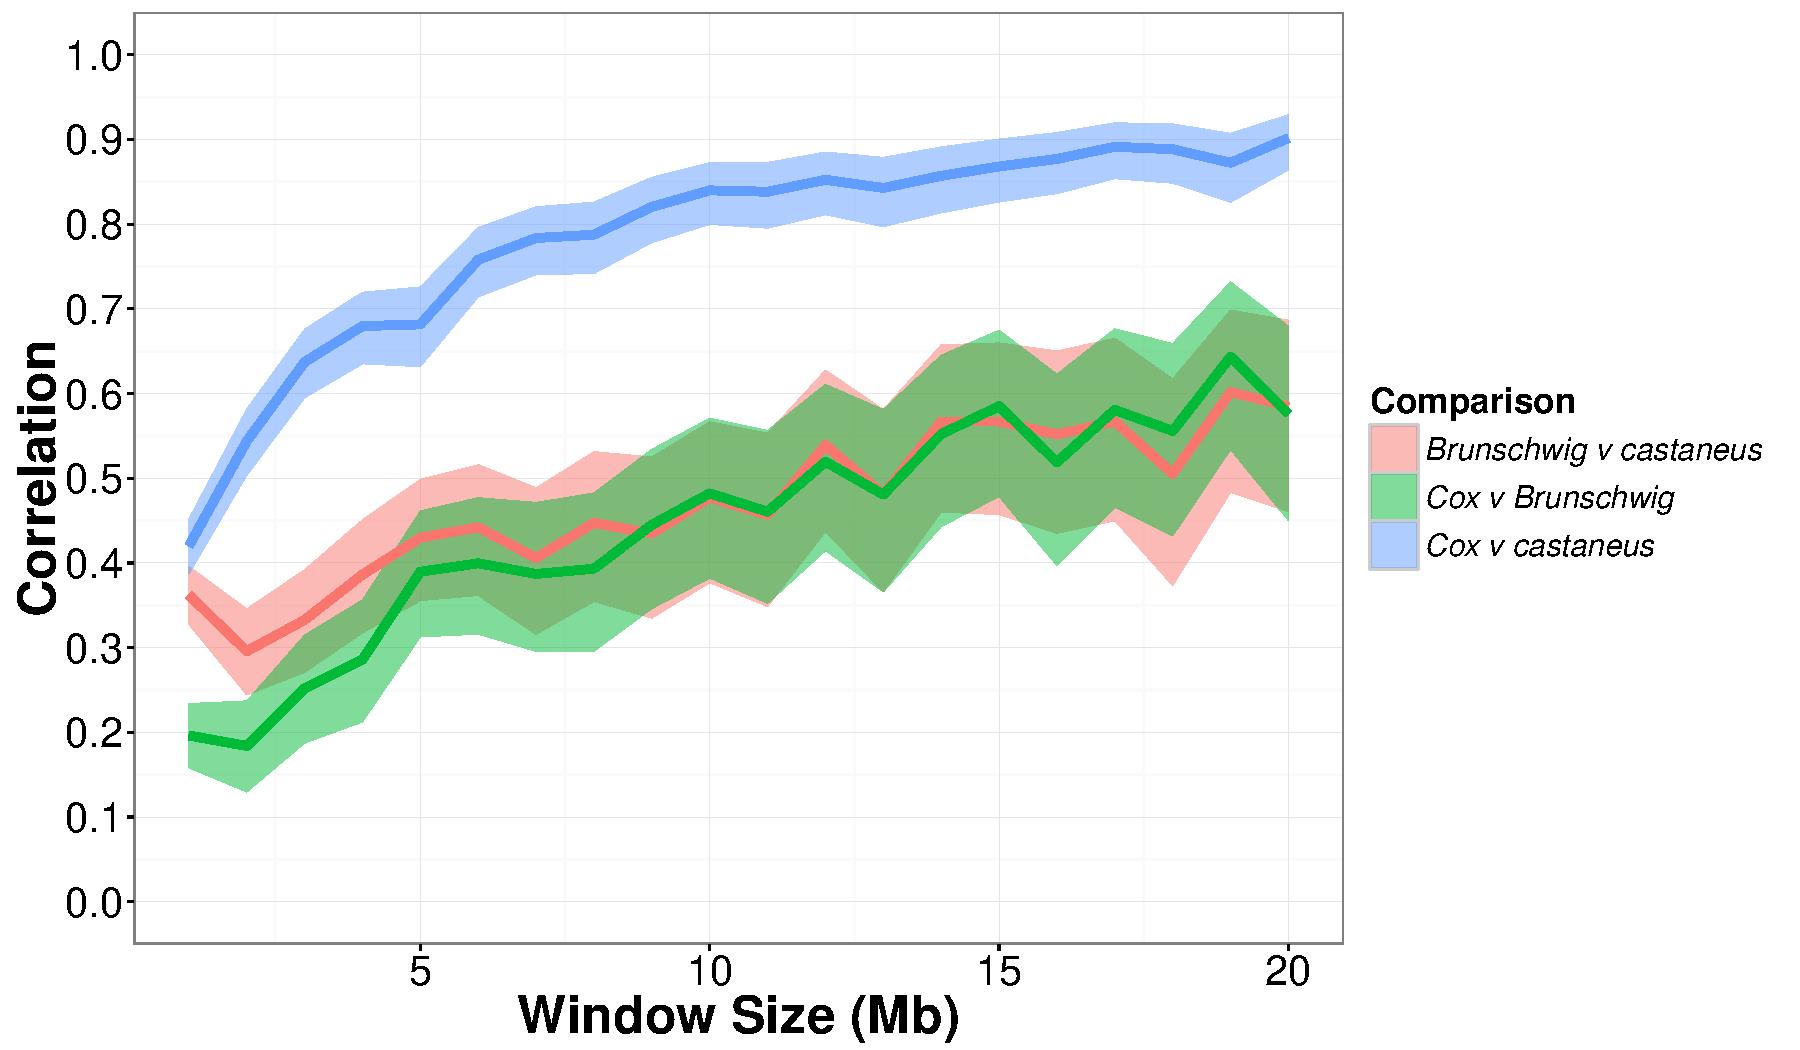
\includegraphics[width=\textwidth]{/Users/s0784966/Dropbox/Thesis/chapter2/Figures/Figure3.pdf}}
 \caption[Broad-scale correlations between recombiantion maps for \emph{Mus musculus castaneus} and \emph{Mus musculus domesticus}]{Pearson correlation coefficients between the recombination map inferred for \emph{M. m. castaneus}, the \cite{RN156} map and the \cite{RN232} map. Correlations were calculated in nonoverlapping windows of varying size across all autosomes. Confidence intervals (95\%) are indicated by shading}
\label{fig:C2F3}
\end{figure}
\linespread{2}

\subsection{Analysis of fine-scale recombination rates }

	To locate potential recombination hotspots in wild \textit{M. m. castaneus}, we generated a fine-scale map, from which we identified 39,972 potential recombination hotspots. For each chromosome, there was an average of 15 hotspots per Mbp. The total number of putative hotspots is more than twice the number identified in CAST/EiJ, an inbred strain derived from wild \textit{M. m. castaneus} \citep{RN249}.

	To obtain a measure of the amount of fine-scale recombination rate heterogeneity across the genome, we constructed Lorenz curves and calculated their Gini coefficients (Figure \ref{fig:C2SF5}). The mean Gini coefficient for all chromosomes was 0.78. This estimate is very similar to that of \cite{RN333} median Gini coefficient of 0.77 for chromosome 1, obtained from a high-density map of crossing-over locations in inbred mice \citep{RN263}. The Gini coefficients calculated from our fine-scale map suggest that the distribution of recombination rates in wild and inbred mice are similarly heterogeneous. However, the Lorenz curve for the X-chromosome is clearly distinct from that of the autosomes (Figure \ref{fig:C2SF5}), and its Gini coefficient is 0.95. 

There was only a small amount of overlap between the locations of putative recombination hotspots we identified in wild \textit{castaneus} and the locations of DSB hotspots observed in wild-derived inbred strains \citep{RN249} (Table \ref{tab:C2ST4}). As may be expected, DSB hotspots in the inbred strain derived from \textit{M. m. castaneus} (CAST) exhibited the greatest amount of overlap with the locations of recombination hotspots identified in \textit{M. m. castaneus}. Of all DSB hotspots in CAST, 12.2\% (or 4.1\% after correcting for the null expectation) overlapped with one of the putative hotspots we identified. Such a low proportion strongly suggests that, even within the \textit{M. m. castaneus} subspecies, the locations of recombination hotspots are highly variable. The PWD strain, which was derived from wild \textit{M. m. musculus}, exhibited the second highest amount of overlap. Less than 1\% of the DSB hotspots in each of the three strains derived from \textit{M. m. domesticus} overlapped with putative hotspots in \textit{M. m. castaneus}, after correcting for the number of overlaps expected to be seen by chance. Table \ref{tab:C2ST4} shows the overlap for each of the strains analysed by \cite{RN249}.

\subsection{Correlation between recombination rate and properties of protein coding genes}

	There is evidence of pervasive natural selection acting in protein-coding genes and conserved non-coding elements of the murid genome \citep{RN158, RN170, RN122}. This is expected to reduce diversity at linked neutral sites via background selection and/or selective sweeps, and is therefore expected to generate a positive correlation between diversity and recombination rate, as has been observed in multiple species \citep{RN117}. 

	We examined the correlation between genetic diversity and recombination rate to determine whether our map captures variation in $N_e$ across the genome. We found that the rate of recombination at autosomal protein-coding genes is significantly and positively correlated with genetic diversity of putatively neutral sites (Table \ref{tab:C2T2}). Furthermore, the correlation between recombination rate and neutral diversity scaled by divergence (from the rat) was both positive and significant, regardless of base context (Table \ref{tab:C2T2}; Figure \ref{fig:C2F2}). This indicates that natural selection may have a role in reducing diversity via hitchhiking and/or background selection.

	Biased gene conversion can influence levels of between-species nucleotide substitution \citep{RN331}. GC-biased gene conversion (gcBGC), where G/C alleles are preferentially chosen as the repair template following double-strand breaks, can generate a positive correlation between nucleotide divergence and recombination rate \citep{RN330}. Gene conversion occurs whether or not a DSB is resolved by crossing-over \citep{RN331} and models of gcBGC predict an increase in the rates of nucleotide substitution in regions of high crossing-over \citep{RN330}. Indeed, human-chimp divergence is positively correlated with rates of crossing-over when considering all base contexts. Consistent with this, we found that 4-fold site nucleotide divergence was significantly positively correlated with recombination rate for the case of all sites (Table \ref{tab:C2T2}). In the case of non-CpG-prone sites, however, we found only a weak negative correlation (Table \ref{tab:C2T2}). A recent study by \cite{RN332} found a positive correlation between human-chimp divergence and recombination rate that persisted after removing CpG-prone sites, so further study is required to analyze the effects of gene conversion on patterns of divergence in mice.

\linespread{1}
%\captionsetup{font=script, labelfont=bf , textfont=it}
\begin{table}[h]



 \begin{tabular}{c c c c } \\[ 0.5ex ]
 \hline 
& \multicolumn{2}{c}{Correlation Coefficient}\\ [0.5ex] \cline{2-3}
& Non-CpG Prone Sites & All Sites\\
\hline
Nucleotide diversity ($\pi$) & 0.090 & 0.20 \\
Divergence from rat ($d_{rat}$) & -0.038 & 0.062 \\
Corrected diversity ($\pi/d_{rat}$) & 0.10 & 0.18 \\
\hline

\end{tabular}
\caption[Correlations between recombination rate and genetic diversity]{Correlation coefficients between recombination rate and pairwise nucleotide diversity and divergence from the rat at fourfold degenerate sites for protein coding genes}
\end{table}

\linespread{2}

\section{Discussion}
 
	Our analyses suggest that the recombination landscapes of wild house mice and their laboratory counterparts are similar at broad-scales, but are dissimilar at fine-scales. Our broad-scale map captures variation in the recombination rate similar to that observed in a more traditional linkage map, both at the level of whole chromosomes and genomic windows of varying sizes. However, we found that a relatively small proportion of double-strand break (DSB) hotspots identified in wild-derived strains \citep{RN249} overlapped with putative recombination hotspots in \textit{M. m. castaneus}. This suggests that recombination rates are highly variable within and between the subspecies at the kilobase scale. We discuss potential reasons for this below.
 
	Recombination landscapes inferred using coalescent approaches, as in this study, reflect ancestral variation in recombination rates. In \textit{M. m. castaneus}, we have shown that this ancestral variation is highly correlated with contemporary recombination rate variation in inbred mice derived from \textit{M. m. domesticus}, suggesting that the broad-scale genetic map has not evolved substantially since the subspecies shared a common ancestor, around 350,000 years ago \citep{RN315}. At a finer scale however, there is considerable variation in the locations of recombination hotspots between the \textit{M. musculus} subspecies. This was also observed in studies of the great-apes, which suggested that the locations of recombination hotspots have strongly diverged between species, but that broad-scale patterns are relatively conserved \citep{RN222, RN221}. There are, however, several relatively large regions of the genome showing substantially different recombination rates between our \textit{M. m. castaneus} map and the Cox map. For example, there are recombination rate peaks in \textit{M. m. castaneus} on chromosomes 4, 5, 14 and 15, which are not present in the Cox map (Figure \ref{fig:C2SF3}). Directly estimating recombination rates at fine scales in \textit{M. m. castaneus} individuals could potentially reveal whether the broad-scale differences in recombination rate, mentioned above, are present in modern day populations. 

The positive correlation between the \textit{castaneus} map and the Cox map (constructed using a pedigree-based approach) is weaker for the X-chromosome than for autosomes of similar physical length (e.g., chromosomes 2 and 3)(Figure \ref{fig:C2SF4}). However, SNP density on the \textit{M. m. castaneus} X-chromosome is substantially lower than the autosomes (Table \ref{tab:C2ST3}). Greater physical distance between adjacent SNPs restricts the resolution of recombination rates in the coalescent-based approach. Thus, in our study, recombination rates are resolved at finer scales on the autosomes than on the X-chromosome. Additionally, we inferred recombination rates on the X-chromosome using 17 gene copies rather than the 20 used for the autosomes. Our findings are consistent, however, with the results of \cite{RN244}, who constructed linkage maps in \textit{M. m. castaneus} and \textit{M. m. musculus} (both by crossing with \textit{M. m. domesticus}) using a small number of markers. In that study, the authors found multiple genomic intervals that significantly differed in genetic map distance between the two subspecies, and a disproportionate number of differences were on the X-chromosome. Thus, their results and ours suggest that the recombination landscape of the X-chromosome has evolved faster than that of the autosomes. 

A recent study by \cite{RN221} examined pairs of great ape species, and found that correlations between recombination maps (at the 1Mbp scale) declined with genetic divergence. For example, between humans and gorillas, genetic divergence is ~1.4\%, while the Spearman-rank correlation of their respective recombination rate maps is ~0.5. Genetic divergence between \textit{M. m. castaneus} and \textit{M. m. domesticus} is reported to be ~0.5\% \citep{RN255}, and we find a Spearman-rank correlation of 0.47 between the \textit{castaneus} map and the Cox map, also at the 1Mbp scale. Although this is only a single data point, it suggests that recombination rate differences may have accumulated faster relative to divergence between \textit{M. m. castaneus} and \textit{M. m. domesticus} than they have between great ape species. The recombination maps constructed for the great apes by \cite{RN221}  were all generated using the same methodology, which is not the case for the comparison we make between our map and that of \cite{RN232}, so quantitative comparisons between the studies should be treated with caution. Performing a comparative analysis of recombination rates in the different subspecies of house mice and related mouse species (for example, \textit{Mus caroli} and \textit{Mus spretus}) using LD-based methods may help us understand whether the rate of evolution of the recombination landscape in wild mice is more rapid than in the great apes.

The locations of the vast majority of recombination hotspots in mice are directed by the binding of the PRDM9 protein \citep{RN254}, and there are unique landscapes of DSB hotspots associated with the different PRDM9 alleles present in different wild-derived inbred strains \citep{RN249}. However, in natural populations there is a great diversity of PRDM9 alleles in each of the \textit{M. musculus} subspecies \citep{RN292}, therefore the binding motif will vary, causing different suites of hotspot locations. Thus, the DSB hotspot maps obtained by \cite{RN249} likely represent a fraction of the diversity of hotspot locations in wild \textit{M. musculus} populations. Indeed, we found that only 12\% of the DSB hotspots reported for CAST/EiJ by \cite{RN249} overlapped with hotspots we inferred for \textit{M. m. castaneus} (Table \ref{tab:C2ST4}). However, the mean Gini coefficient we estimated for \textit{M. m. castaneus} was almost identical to the value obtained by \cite{RN333} from crossing-over data of \textit{M. musculus}. This similarity suggests that while the locations of hotspots may differ, the distribution of recombination rates is similarly heterogeneous in wild and inbred mice.

The \textit{castaneus} map constructed in this study appears to be more similar to the Cox map than the Brunschwig map (Figure \ref{fig:C2F3}). There are number of potential reasons for this. Firstly, we used a much larger number of markers to resolve recombination rates than \cite{RN156}. Secondly, it seems probable that population structure within and between the inbred and wild-derived lines studied by \cite{RN156} could have resulted in biased estimates of the recombination rate. The Brunschwig map does, however, capture true variation in the recombination rate, since their map is also highly correlated with the Cox map (Pearson correlation >0.4) for all genomic windows wider than 8Mbp (Figure \ref{fig:C2F3}). Indeed, \cite{RN156} showed by simulation that hotspots are detectable by analysis of inbred lines, and validated their hotspots against the locations of those observed in crosses among classical strains of \textit{M. m. domesticus} \citep{RN180}. This suggests that while estimates of the recombination rate in the \cite{RN156} map may have been downwardly biased by population structure (see above), variation in the rate and locations of hotspots were still accurately detected.
 
By simulating the effect of switch errors on estimates of the recombination rate, we inferred the range over which $\rho$/bp is accurately estimated. Switch errors appear identical to legitimate crossing-over events and, if they are randomly distributed along chromosomes, a specific rate of error will resemble a constant rate of crossing-over. The rate of switch error will then determine a detection threshold below which recombination cannot be accurately inferred. We investigated this detection threshold by introducing switch errors, at random, into simulated data at the rate we estimated using the X-chromosome. We found that, in the presence of switch errors, LDhelmet consistently overestimates the recombination rate when the true value is below 2 x $10^{-3}$ $\rho /bp$ (Figure \ref{fig:C2F1}; Figure \ref{fig:C2SF1}). This highlights a possible source of bias affecting LD-based recombination mapping studies that use inferred haplotypes, and suggests that error in phase inference needs to be carefully considered.

        	We obtained an estimate of the switch error rate, using a novel approach that took advantage of the hemizygous sex chromosomes of males. This allowed us to assess the extent by which switch errors affected our ability to infer recombination rates. Our inferred switch error rate may not fully represent that of the autosomes, however, because multiple factors influence the ability to phase variants (i.e., LD, SNP density, sample size, depth of coverage and read length), and some of these factors differ between the X-chromosome and the autosomes. The sex-averaged recombination rate for the X-chromosome is expected to be 3/4 that of the autosomes, so it will likely have elevated LD, and thus there will be higher power to infer phase. In contrast, X-linked nucleotide diversity in \textit{M. m. castaneus} is approximately one-half that of the autosomes \citep{RN238}, so there would be a higher number of phase informative reads on the autosomes. While it is difficult to assess whether the switch error rates we estimated from the X-chromosome will be similar to those on the autosomes, the analysis allowed us to explore the effects of different SNP filters on the error rate.
 
	Consistent with studies in a variety of organisms \citep{RN117}, we found a positive correlation between genetic diversity at putatively neutral sites and the rate of recombination. Both unscaled nucleotide diversity and diversity divided by divergence between mouse and rat, a proxy for the mutation rate, are positively correlated with the recombination rate (Table \ref{tab:C2T2}). \cite{RN168} found evidence suggesting that recombination may be mutagenic, although insufficient to account for the correlations they observed. The Kendall correlation between $\pi/d_{rat}$ and recombination rate is 0.20 for all 4-fold sites (Table \ref{tab:C2T2}), which is similar in magnitude to the corresponding value of 0.09 reported by \cite{RN168} in humans. The correlations we report may be downwardly biased, however, because switch errors may result in inflated recombination rates for genomic regions where the recombination rate is low (see above). Genes that have recombination rates lower than the detection limit set by the switch error rate may be reported as having inflated $\rho /bp$ (Figure \ref{fig:C2F1}; Figure \ref{fig:C2SF1}), and this would have the effect of reducing correlation statistics. It is difficult to assess the extent of this bias, however, and in any case the correlations we observed between diversity and recombination suggest that our recombination map does indeed capture real variation in $N_e$ across the genome. This indicates that a recombination mediated process influences levels of genetic diversity. Previously, \cite{RN122} showed that there are reductions in nucleotide diversity surrounding protein coding exons in \textit{M. m. castaneus}, characteristic of natural selection acting within exons reducing diversity at linked sites. Their results and ours suggest pervasive natural selection in the \textit{M. m. castaneus} genome. In contrast, a previous study in wild mice found that, while \textit{M. m. musculus} exhibited a significant correlation between diversity and recombination, the relationship was non-significant for both \textit{M. m. castaneus} and \textit{M. m. domesticus} \citep{RN315}. This study analysed only 27 loci, so was perhaps underpowered to detect a relatively weak correlation. It should be noted, however, that the measure of recombination rate we used ($\rho /bp$) and neutral genetic diversity are both functions of the effective population size, so the positive correlation we detected could be partly driven by random fluctuations of $N_e$ across the genome.

	Furthering our understanding of the evolution of the recombination landscape in house mice would be helped by comparing fine-scale rates in the different subspecies. In this study we have assumed that inbred lines derived from \textit{M. m. domesticus} reflect natural variation in recombination rates in that subspecies, though this is not necessarily the case. Directly comparing natural population samples of the different subspecies may help reconcile several potentially conflicting results. For example, the hotspots we detected in our study show more overlap with \textit{M. m. musculus} than with \textit{M. m. domesticus}, based on the DSB hotspots reported by \cite{RN249}. However, overall rates of crossing-over in male \textit{M. m. musculus} are higher than in either \textit{M. m. castaneus} or \textit{M. m. domesticus} \citep{RN270}. Additionally, there is evidence of recombination rate modifiers of large effect segregating within \textit{M. m. musculus} populations \citep{RN244}. So, although overall rates of crossing-over in \textit{M. m. musculus} are higher than in the other species, its recombination landscape may be more similar to \textit{M. m. castaneus} than to \textit{M. m. domesticus}. A broad survey comparing recombination rate landscapes in the different subspecies of mice would most efficiently be performed using LD-based approaches.  

In conclusion, we find that sex-averaged estimates of the ancestral recombination landscape for \textit{M. m. castaneus} are highly correlated with contemporary estimates of the recombination rate observed in crosses of inbred lines that predominantly reflect \textit{M. m. domesticus} \citep{RN232}. It has previously been demonstrated that the turnover of hotspots has led to rapid evolution of fine-scale rates of recombination in the \textit{M. musculus} subspecies complex \citep{RN249} and our results suggest that even within \textit{M. m. castaneus} hotspot locations are variable. On a broad scale, however, our results suggest that the recombination landscape is very strongly conserved between \textit{M. m. castaneus} and \textit{M. m. domesticus} at least. In addition, our estimate of the switch-error rate implies that phasing errors lead to upwardly biased estimates of the recombination rate when the true rate is low. This is a source of bias that should be assessed in future studies. Finally, we showed that the variation in recombination rate is positively correlated with genetic diversity, suggesting that natural selection reduces diversity at linked sites across the \textit{M. m. castaneus} genome, consistent with the findings of \cite{RN122}. 
  
	% Boot up the Chapter 3: Introduction file
	\chapter{Understanding the factors that shape patterns of nucleotide diversity in the house mouse genome}
\chaptermark{Selection at linked sites in wild mice}

\externaldocument{\dir/chapter3Appendix/chapter3appendix.tex}

\section{Abstract}
	A major goal of population genetics has been to determine the extent by which selection at linked sites influences patterns of neutral nucleotide diversity in the genome. Multiple lines of evidence suggest that diversity is influenced by both positive and negative selection. For example, in many species there are troughs in diversity surrounding functional genomic elements, consistent with the action of either background selection (BGS) or selective sweeps. In this study, we investigated the causes of the diversity troughs that are observed in the wild house mouse genome. Using the unfolded site frequency spectrum (uSFS), we estimated the strength and frequencies of deleterious and advantageous mutations occurring in different functional elements in the genome. We then used these estimates to parameterize forward-in-time simulations of chromosomes, using realistic distributions of functional elements and recombination rate variation in order to determine if selection at linked sites can explain the observed patterns of nucleotide diversity. The simulations suggest that BGS alone cannot explain the dips in diversity around either exons or conserved non-coding elements (CNEs). A combination of BGS and selective sweeps produces deeper dips in diversity than BGS alone, but the inferred parameters of selection cannot fully explain the patterns observed in the genome. Our results provide evidence of sweeps shaping patterns of nucleotide diversity across the mouse genome, and also suggest that infrequent, strongly advantageous mutations play an important role in this. The limitations of using the uSFS for inferring the frequency and effects of advantageous mutations are discussed.

\section{Introduction}
 
	Starting with the discovery of a positive correlation between nucleotide polymorphism and the recombination rate in \textit{Drosophila} in the late 1980s and early 1990s \citep{RN225, RN114}, it has become clear that natural selection affects genetic diversity across the genomes of many species \citep{RN117, RN154}. More recently, models incorporating selection at sites linked to those under observation have been shown to explain a large amount of the variation in diversity across the genome \citep{RN120, RN228, RN116, RN274}. However, a persistent challenge has been to tease apart the contributions of positive and negative selection to the observed patterns.

	Because the fates of linked alleles are non-independent, selection acting at one site may have consequences for variation and evolution at another. In broad terms, there are two models describing the effects of directional selection on neutral genetic diversity at linked sites, selective sweeps (SSWs) and background selection (BGS). SSWs occur when positively selected alleles spread through a population, dragging with them the haplotype on which they arose \citep{RN124,RN235}. There are a number of different types of SSW (reviewed in \citealt{RN352}), but in the present study, when not made explicit, we use the term selective sweep to refer to the effects of a single de novo advantageous mutation being driven to fixation by selection. BGS, on the other hand, occurs because the removal of deleterious mutations results in a loss of genetic diversity at linked neutral sites \citep{RN132, RN115}. The magnitudes of the effects of SSWs and BGS depend on the strength of selection, the rate of recombination and the mutation rate \citep{RN206, RN157, RN235}. SSWs and BGS have qualitatively similar effects on genetic diversity, however, and many polymorphism summary statistics have little power to distinguish between them \cite{RN339, RN115}. 

	Several studies have attempted to differentiate between BGS and SSWs. For example, \cite{RN167} examined patterns of nucleotide diversity around recent nucleotide substitutions in \textit{Drosophila simulans}. Averaging across the entire genome, they observed a trough in diversity around nonsynonymous substitutions, whereas diversity was relatively constant around synonymous ones. This difference is expected under a model of recurrent SSWs, but not under BGS. Their results provide evidence that SSWs have been frequent in \textit{D. simulans} since the species shared a common ancestor with \textit{Drosophila melanogaster} (the outgroup used in that study). Similar results have been reported for \textit{Capsella grandiflora} \citep{RN236}. In humans \citep{RN162}, house mice \citep{RN122} and maize \citep{RN230}, however, there is very little difference between the patterns of diversity around putatively neutral and potentially adaptive substitutions. These results have been interpreted as evidence that hard SSWs are infrequent in those species. However, \cite{RN237} argued that the proportion of neutral amino acid substitutions in regions of the genome with low functional constraint (and thus weak BGS effects) will be higher than the proportion occurring in regions with high functional constraint (and thus stronger BGS effects), so the Sattath test will be difficult to interpret in species with genomes exhibiting highly variable levels of functional constraint, such as humans and mice (but see \citealt{RN230}). Indeed, \cite{RN237} found evidence that adaptive substitutions are fairly frequent in both protein-coding and non-coding portions of the human genome, suggesting that SSWs are common. Furthermore, \cite{RN365} analysed reductions in nucleotide diversity in genomic regions close to genes in the great apes and concluded that strong SSWs, rather than BGS, are required to explain the observed patterns. In that study, although the authors examined a wide range of selection parameters, they did not attempt to identify parameters of selection specific to any ape species.

	There are a number of methods for estimating the frequency and strength of advantageous mutations using models of selection at linked sites \citep{RN352}. Recently, \cite{RN274} produced a map of the expected nucleotide diversity in \textit{D. melanogaster} by fitting a model incorporating both BGS and hard SSWs to the genome-wide patterns of genetic diversity and the divergence between \textit{D. melanogaster} and \textit{D. simulans}. They concluded that sweeps are required to explain much of the genome-wide variation in diversity. Their analysis conditioned the effects of sweeps on the locations of recent substitutions, which is reasonable in \textit{D. melanogaster} where there is a reduction in mean diversity around nonsynonymous substitutions, but not around synonymous ones \citep{RN274}. As described above, this is not the case for wild mice. Indeed, even randomly selected synonymous and nonsynonymous sites in \textit{Mus musculus}, regardless of whether they have experienced a recent substitution, exhibit almost identical reductions in diversity in surrounding regions \cite{RN122}. Conditioning a sweep model on the locations of recent substitutions in mice may, therefore, produce spurious parameter estimates. Furthermore, the selection parameters estimated by \cite{RN122} were inferred solely from variation in nucleotide diversity. There is information in the distribution of allele frequencies, the site frequency spectrum (SFS), that can be used to estimate the distribution of fitness effects (DFE) for both deleterious and advantageous mutations \citep{RN164, RN201, RN210, RN354}. In the present study, we estimate the DFE using such methods, and then use our estimates to parameterise simulations modelling BGS and SSWs.

	In this study, we attempt to understand the influence of natural selection on variation at linked sites in the house mouse, \textit{Mus musculus}. Specifically, we analyse \textit{M. m. castaneus}, a sub-species which has been estimated to have a long-term effective population size ($N_e$) of around 500,000 \citep{RN233, RN158}, making it a powerful system in which to study molecular evolution in mammals. Both protein-coding genes and phylogenetically conserved non-coding elements (CNEs, which have roles in the regulation of gene expression \citep{RN353}) exhibit signatures of natural selection in \textit{M. m. castaneus} \citep{RN122}. In particular, \cite{RN122} showed that there are substantial reductions in diversity surrounding protein-coding exons and CNEs, consistent with selection reducing diversity at linked sites. The trough in diversity surrounding exons was found to be ~10x wider than the trough surrounding CNEs, suggesting that selection is typically stronger on protein sequences than regulatory sequences. These results, therefore, suggest that selection at linked sites affects nucleotide diversity across large portions of the genome. However, our understanding of the forces that have shaped patterns of diversity is incomplete.

	We analyse data on wild-caught \textit{M. m. castaneus} individuals to obtain estimates of the distribution of fitness effects (DFE) for several classes of functional elements in the mouse genome and then use these to parametrise forward-in-time simulations. We analyse several aspects of our simulation data: 1) the patterns of genetic diversity and the distribution of allele frequencies around both protein-coding exons and conserved non-coding elements; 2) the rates of substitution in different functional elements; and 3) the patterns of diversity around nonsynonymous and synonymous substitutions.
\section{Materials and Methods}

\subsection{Samples and polymorphism data}
 
	We analysed the genome sequences of 10 wild-caught \textit{M. m. castaneus} individuals sequenced by \cite{RN122}. The individuals were sampled from an area that is thought to include the ancestral range of the species\citep{RN233}. A population structure analysis suggested that the individuals chosen for sequencing came from a single randomly mating population \citep{RN158}. Sampled individuals were sequenced to an average depth of ~30x using Illumina technology. Reads were mapped to version mm9 of the mouse genome and variants called as described in \cite{RN122}. Only single nucleotide polymorphisms were considered, and insertion/deletion polymorphisms were excluded from downstream analyses. We used the genome sequences of \textit{Mus famulus} and \textit{Rattus norvegicus} as outgroups in this study. For \textit{M. famulus}, a single individual was sequenced to high coverage and mapped to the mm9 genome \citep{RN122}. For \textit{R. norvegicus}, we used the whole genome alignment of the mouse (mm9) and rat (rn4) reference genomes from UCSC. 

	For the DFE-alpha analysis (see below), the underlying model assumes a single, constant mutation rate. Hypermutable CpG sites strongly violate this assumption, so CpG-prone sites were excluded as a conservative way to remove CpG sites from our analyses. A site was labelled as CpG-prone if it is preceded by a C or followed by a G in the 5’ to 3’ direction in either \textit{M. m. castaneus}, \textit{M. famulus} or \textit{R. norvegicus}. Additionally, sites that failed a Hardy-Weinberg equilibrium test (p < 0.002) were excluded from further analysis, because they may represent alignment errors.
 
\subsection{Functional elements in the murid genome}
        
	In this study, we considered three different classes of functional elements in the genome: the exons and untranslated regions (UTRs) of protein-coding genes and conserved non-coding elements (CNEs).

	Coordinates for canonical splice-forms of protein-coding gene orthologs between \textit{Mus musculus} and \textit{Rattus norvegicus} were obtained from version 67 of the Ensembl database. We used these to identify untranslated regions (UTRs) as well as 4-fold and 0-fold degenerate sites in the coding regions. We made no distinction between 3’ and 5’ UTRs in the analysis. Genes containing alignment gaps affecting >80\% of sites in either outgroup and genes containing overlapping reading frames were excluded. This left a total of 18,171 autosomal protein-coding genes.
 
	The locations of conserved non-coding elements (CNEs) in the house mouse genome were identified as described by \cite{RN122}. 

Estimating the parameters of the distribution of fitness effects (DFE) for a particular class of sites using DFE-alpha (see below) requires neutrally evolving sequences for comparison. When analysing 0-fold degenerate sites and UTRs, we used 4-fold degenerate sites as the comparator. For CNEs, we used non-conserved sequence in the flanks of CNEs. \citep{RN122} found that, compared to the genome-wide average, nucleotide divergence between mouse and rat in the ~500bp on either side of CNEs is ~20\% lower than that of intergenic DNA distant from CNEs, suggesting functional constraint in these regions. For the purpose of obtaining a quasi-neutrally evolving reference class of sequence and to avoid these potentially functional sequences, we therefore used sequence flanking the edges of each CNE, offset by 500bps. For each CNE, the total amount of flanking sequence used in the analysis was equal to the length of the focal CNE, split evenly between the upstream and downstream regions. CNE-flanking sequences overlapping with another annotated feature (i.e. exon, UTR or CNE) or the flanking sequence of another CNE were excluded.

\subsection{The site frequency spectrum around functional elements}
 
	For distances of up to 100Kbp on either side of exons and 5Kbp on either side of CNEs, the non-CpG-prone sites in non-overlapping windows of 1Kbp and 100bp, respectively, were extracted. For each analysis window, we calculated the genetic distance to the focal element in terms of the population-scaled recombination rate ($\rho = 4N_er$) using the \textit{M. m. castaneus} recombination map we constructed in an earlier study \citep{RN340}. Sites within analysis windows that overlapped with any of the annotated features described above, or that contained missing data in \textit{M. m. castaneus} or either outgroup were excluded. The data for analysis windows were collated based on either physical or genetic distances distance from the nearest CNE or exon, from which we calculated nucleotide diversity and Tajima’s $D$.

\subsection{Overview of DFE-alpha analysis}

	The distribution of allele frequencies in a sample, referred to as the site frequency spectrum (SFS), provides information on evolutionary processes. Under neutrality the SFS reflects past demographic processes, such as population expansions and bottlenecks, and potentially the effects of selection at linked sites. The allele frequency distribution will also be distorted if focal sites are subject to functional constraints. The SFS therefore contains information on the strengths and frequencies of mutations with different selective effects, known as the distribution of fitness effects (hereafter the DFE). Note that balancing selection may maintain alleles at intermediate frequencies \citep{RN103}, but we assume that the contribution of this form of selection to overall genomic diversity is negligible.

	DFE-alpha estimates selection parameters using information contained in the SFS by a two-step procedure \citep{RN164}. First, a demographic model is fitted to data for a class of putatively neutral sites. Conditional on the demographic parameter estimates, the DFE is then estimated for the selected sites. In the absence of knowledge of ancestral or derived alleles, the ‘folded’ SFS can be used to estimate the demographic model and the DFE for harmful variants (hereafter referred to as the dDFE) \citep{RN164}. If information from one or more outgroup species is available, and the ancestral state for a segregating site can be inferred, one can construct the ‘unfolded’ SFS (uSFS). In the presence of positive selection, such that advantageous alleles segregate at an appreciable frequency, the parameters of the distribution of fitness effects for advantageous mutations can be estimated from the uSFS \citep{RN210, RN321, RN354}. In this study, we estimate the proportion of new mutations occurring at a site that are advantageous ($p_a$) and the strength of selection acting on them ($N_es_a$).

\subsection{Inference of the uSFS and the DFE}
 
	We inferred the distributions of derived allele frequencies in our sample for 0-fold and 4-fold sites, UTRs, CNEs and CNE-flanks using \textit{M. famulus} and \textit{R. norvegicus} as outgroups, using the two-outgroup method implemented in ml-est-sfs v1.1 \citep{RN321}. This method employs a two-step procedure conceived to address the biases inherent in parsimony methods. The first step estimates the rate parameters for the tree under the Jukes-Cantor model by maximum likelihood assuming a single mutation rate. Conditional on the rate parameters, the individual elements of the uSFS are then estimated.
 
	DFE-alpha fits discrete population size models, allowing up to two changes in population size through time. For each class of putatively neutral sites, one-, two- and three-epoch models were fitted by maximum likelihood and the models with the best fit (as judged by likelihood ratio tests) were used in further analyses. When fitting the three-epoch model, we ran DFE-alpha (v2.16) 10 times with a range of different search algorithm starting values, in order to check convergence. We explored the effect of fitting the demographic model to a smaller number of individuals by down-sampling the 4-fold sites dataset to 5 and 8 individuals, with respect to frequency.

	In the cases of 4-fold sites and CNE-flanks, the inferred uSFSs exhibited a higher proportion of high frequency derived alleles than expected under the best-fitting demographic model (Figure \ref{fig:C3S1}) (hereafter referred to as an uptick). Such an increase is not possible under the single population, single locus demographic models assumed. There are several possible explanations for the uptick: 1) mis-inference of the uSFS due to an inadequacy of the model assumed in ml-est-sfs; 2) failure to capture the demographic history of \textit{M. m. castaneus} by the models implemented in DFE-alpha; 3) sequencing errors in \textit{M. m. castaneus} or either outgroup generating spurious signals of divergence; 4) SSWs, since they can drag linked alleles to high frequencies \citep{RN287,RN343}; 5) cryptic population sub-division in our sample of mouse individuals; and 6) positive selection, acting on the putatively neutral sites themselves. We think this latter explanation is unlikely, however, since there is little evidence for selection on synonymous codon usage in \textit{Mus musculus} \citep{RN195}. With the exception of direct selection affecting the putatively neutral class of sites, the above sources of bias should also affect the selected class of sites \citep{RN275, RN276, RN321}. We therefore corrected the selected sites uSFS prior to inferring selection parameters by subtracting the proportional deviation between the neutral uSFS expected under the best-fitting demographic model and the observed neutral uSFS (following \citealt{RN321}; see Supplementary Methods). 
 
	Simultaneous inference of the DFE for harmful mutations (dDFE) and adaptive mutation parameters was performed using DFE-alpha (v.2.16) \citep{RN210}. A gamma distribution has previously been used to model the dDFE, since it can take a variety of shapes and has only two parameters \citep{RN109}. However, more parameter-rich discrete point mass distributions provide a better fit to nonsynonymous polymorphism site data in wild house mice \citep{RN178}. We therefore compared the fit of one, two and three discrete class dDFEs and the gamma distribution, and also included one or more classes of advantageous mutations. Nested DFE models were compared using likelihood ratio tests, and non-nested models were compared using Akaike’s Information Criteria (AIC). Goodness of fit was also assessed by comparing observed and expected uSFSs using the $\chi^2$ ­statistic, but the numbers of sites in the $i^{th}$ and $n-i^{th}$ classes are non-independent, so formal hypothesis tests were not performed.

	We constructed profile likelihoods to obtain confidence intervals. Two unit reductions in $logL$, on either side of the maximum likelihood estimates (MLEs) were taken as approximate 95\% confidence limits. 

\subsection{Two methods for inferring the rates and effects of advantageous mutations based on the uSFS}

	It has been suggested that estimates of the DFE obtained based on the uSFS may be biased if sites fixed for the derived allele are included in calculations \cite{RN354}. Sites fixed for the derived allele are typically a frequent class in the uSFS, and therefore strongly influence parameter estimates. Bias can arise, for example, if the selection strength has changed since the split with the outgroup, such that the number of sites fixed for the derived allele do not reflect the selection regime that generated current levels of polymorphism. If nucleotide divergence and polymorphism are decoupled in this way, selection parameter estimated from only polymorphism data (and sites fixed for ancestral alleles) may therefore be less biased than those obtained when using the full uSFS. To investigate this possibility, we estimated selection parameters either utilising the full uSFS (we refer to this method as Model A) or by analysing the uSFS while fitting an additional parameter (Supplementary Methods), such that sites fixed for the derived allele do not contribute to estimates of the selection parameters (we refer to this method as Model B). 

Certain alleles present in a sample of individuals drawn from a population may appear to be fixed that are, in fact, polymorphic. Attributing such polymorphisms to between-species divergence may then influence estimates of the DFE by increasing the number of sites fixed for the derived allele (note that this would only affect estimates obtained under Model A). We corrected the effect of polymorphism attributed to divergence using an iterative approach as follows. When fitting selection or demographic models, DFE-alpha produces a vector of expected allele frequencies. Using this vector, we inferred the expected proportion of polymorphic sites that appear to be fixed for the derived allele. This proportion was then subtracted from the fixed derived class and distributed among the polymorphism bins according to the allele frequency vector. We then refitted the model using this corrected uSFS, and this procedure was applied iteratively until convergence (See Supplementary Methods). For each site class, convergence was achieved within five iterations and the selection parameters for each class did not substantially change between iterations. 
	
\subsection{Forward-in-time simulations modelling background selection and selective sweeps}
 
We performed forward-in-time simulations in SLiM v1.8 \citep{RN148} to assess whether the observed patterns of diversity around functional elements \citep{RN122} can be explained by SSWs or BGS caused by mutations originating in the elements themselves. These simulations focussed on either protein-coding exons or CNEs. We also ran SLiM simulations to model the accumulation of between-species divergence under our estimates of the DFE. In all our simulations, we either assumed the estimates of selection parameters obtained from the full uSFS (Model A) or those obtained when sites fixed for the derived allele do not contribute to parameter estimates (Model B).

Models of BGS and recurrent SSWs predict that the magnitudes of their effects are sensitive to the rate of recombination and mutation rate and the strength of selection \citep{RN277, RN157, RN226}. To parameterise our simulations, we used estimates of compound parameters scaled by Ne. For example, estimates of selection parameters obtained from DFE-alpha are expressed in terms of $N_es$ (where $s$ is the difference in fitness between homozygotes for ancestral and derived alleles, assuming semi-dominance). For a population where $N_e$ = 1,000 and $s$ = 0.05, for example, the strength of selection is therefore approximately equivalent to that of a population where $N_e$ = 10,000 and $s$ = 0.005. By scaling parameter values according to the population size of the simulations ($N_{sim}$), we modelled the much larger \textit{M. m. castaneus} population ($N_e$ ~ 500,000; \citealt{RN315}) in a computationally tractable way. However, this linear scaling can be problematic, particularly for strong positive selection \citep{RN198}. We compared patterns of diversity in simulations with population sizes of $N_{sim}$ = 100, 500, 750, 1,000 and 2,000 diploid individuals to assess the effect of the linear scaling given the selection, recombination and mutation parameters we assumed.

\subsubsection{1. Annotating simulated chromosomes}

	Functional elements are non-randomly distributed across the house mouse genome. For example, protein-coding exons are clustered into genes and CNEs are often found close to other CNEs \citep{RN122}. Incorporating this distribution into simulations is important when modelling BGS and recurrent SSWs, because their effects on neutral diversity depend on the density of functional sequence \citep{RN157,RN290}. We incorporated the distribution as follows. For each simulation replicate, we chose a random position on an autosome, which was itself randomly selected (with respect to length). The coordinates of the functional elements (exons, UTRs and CNEs) in the 500Kbp downstream of that position were used to annotate a simulated chromosome of the same length. For simulations focussing on exons (CNEs), we only used chromosomal regions that had at least one exon (CNE).

\subsubsection{2. Mutation, recombination and selection in simulations}
 
	We used an estimate of the population scaled mutation rate, $\theta = 4N_e \mu$, to set the mutation rate ($\mu$) in simulations, such that levels of neutral polymorphism approximately matched those of \textit{M. m. castaneus}. Diversity at putatively neutral sites located close to functional elements (for example, 4-fold synonymous sites) may be affected by BGS and SSWs. To correct for this, we used an estimate of $\theta$ = 0.0083, based on the average nucleotide diversity at non-CpG-prone sites at distances >75Kbp from protein-coding exons. This distance was used, because it the approximate distance beyond which nucleotide diversity remains flat. The mutation rate in simulations was thus set to 0.0083/$4N_{sim}$. 

	Variations in the effectiveness of selection at linked sites, due to variation in the rate of recombination across the genome, may not be captured by simulations that assume a single rate of crossing over. Recently, we generated a map of variation in the rate of crossing-over for \textit{M. m. castaneus} using a coalescent approach \citep{RN340}, quantified in terms of the population scaled recombination rate $\rho = 4N_er$. Recombination rate variation in the 500Kbp region used to obtain functional annotation was used to specify the genetic map for individual simulations. 

	We modelled natural selection at sites within protein-coding exons, UTRs and CNEs in the simulations using the estimates of selection parameters obtained from the DFE-alpha analysis. In the case of protein-coding exons, 25\% of sites were set to evolve neutrally (i.e. synonymous sites), and the fitness effects of the remaining 75\% were drawn from the DFE inferred for 0-fold sites (hereafter termed nonsynonymous sites in the simulations). For mutations in UTRs and CNEs, 100\% were drawn from the DFEs inferred for those elements. Population scaled selection coefficients were divided by $2N_[sim]$ to obtain values of $s$ for use in simulations. All selected mutations were assigned a dominance coefficient of 0.5, as assumed by DFE-alpha.
 
\subsubsection{3. Patterns of diversity around functional elements in simulations}
 
We examined the contributions of BGS and recurrent SSWs to the troughs in diversity observed around protein-coding exons and CNEs using forward-in-time simulations. Focussing on either protein-coding exons or CNEs, we performed three sets of simulations. The first incorporated only harmful mutations (causing BGS), the second only advantageous mutations (causing SSWs), and the third set incorporated both (causing both processes). Thus, under a given set of DFE estimates, we performed six sets of simulations (three sets focussing on exons and three sets focussing on CNEs). For each simulation set, 2,000 SLiM runs were performed, each using a randomly sampled 500Kbp region of the genome. In each SLiM run, populations of $N_[sim]$ = 1,000 diploid individuals were allowed to evolve for 10,000 generations ($10N_[sim]$) in order to approach mutation-selection-drift balance. At this point, 200 randomly chosen haploid chromosomes were sampled from the population and used to construct SFSs.
 
For each set of simulations, segregating sites in windows surrounding functional elements were analysed in the same way as for the \textit{M. m. castaneus} data (see above). The SFSs for all windows at the same distance from an element were collated. Analysis windows around protein-coding exons were oriented with respect to the strand orientation of the actual gene. Neutral sites near the tips of simulated chromosomes only experience selection at linked sites from one direction, so analysis windows located within 60Kbp of either end of a simulated chromosome were discarded. For a given distance to a functional element, we obtained confidence intervals around individual statistics by bootstrapping analysis window 1,000 times.

Mutation rate variation is expected to contribute to variation in nucleotide diversity. Nucleotide divergence between mouse and rat is relatively constant in the intergenic regions surrounding protein-coding exons \citep{RN122}, suggesting that mutation rate variation is not responsible for the troughs in diversity around exons. Around CNEs, however, there is a pronounced dip in nucleotide divergence between \textit{M. m. castaneus} and the rat. A likely explanation for this is that alignment-based approaches to identify CNEs fail to identify the edges of some elements, resulting in the inclusion of functionally constrained sequence in the analysis windows close to CNEs. This factor was not incorporated in our simulations, so in order to correct for this constraint, allowing us to compare diversity around CNEs in \textit{M. m. castaneus} with our simulation data, we scaled values as follows. We divided nucleotide diversity by between-species divergence, in this case mouse-rat divergence, giving a statistic ($\pi/d_[rat]$) that reflects diversity corrected for mutation rate variation. We then multiplied the π/drat values by the mean mouse-rat divergence in regions further than 3Kbp from the edges of CNEs to obtain values on the same scale as our simulation data.

When comparing the patterns of diversity around functional elements in our simulations with the observations from \textit{M. m. castaneus}, we used the root mean square (RMS) as a measure of goodness-of-fit. 
\begin{equation}
RMS = \sqrt{  \frac{1}{n_w}  \sum_{i=1}^{n_w} (\pi_{sim,i} - \pi_{obs,i})^2  }
\end{equation}

where $\pi_{sim,i}$ and $\pi_{obs,i}$ are the diversity values from simulations and \textit{M. m. castaneus}, respectively, in window i around a particular class of functional element and $n_w$ is the total number of analysis windows. Approximate confidence intervals for RMS values were obtained using the bootstrap replicates described above.

\subsubsection{4. Re-inferring the DFE based on simulated population data}

	We performed two additional sets of simulations to model the accumulation of between-species nucleotide divergence under the DFE estimates obtained by analysis of the full uSFS (i.e. Model A) and those obtained when sites fixed for the derived allele did not contribute to selection parameters (i.e. Model B). These simulations were the same as those described above, except that we ran them for additional generations to approximate the mouse-rat divergence. We ran 4,000 replicates of these simulations. Using polymorphic sites and sites fixed for the derived allele, we constructed the uSFS for each class of functional sites. 

	In order to model the mouse-rat divergence, we required a time frame to approximate the neutral divergence between those two species. Neutral divergence between \textit{M. m. castaneus} and \textit{R. norvegicus} ($K_{rat}$) is ~15\% at non-CpG-prone sites far from protein-coding exons. Under neutrality, divergence is expected to be equal to $2T\mu$, where $T$ is the time in generations since the two-species shared a common ancestor and $\mu$ is the mutation rate per base pair per generation. In the simulations, the mutation rate was 2.075 x $10^{-6}$ $bp^{-1}$ (recall that we scaled mutations rates using an estimate of $4N_e\mu$) and since $K_[rat]$ = 0.15, $T$ = 36,145 generations. We thus ran simulations incorporating both deleterious and advantageous mutations, focussing on exons, for 46,145 generations, discarding the first 10,000 as burn-in. At the final generation, we constructed the uSFS for synonymous and nonsynonymous sites from 20 randomly sampled haploid chromosomes. To obtain a proxy for mouse-rat divergence, we counted all substitutions that occurred after the $10N_{sim}$ burn-in phase plus any derived alleles present in all 20 haploid chromosomes.

	Using the uSFSs for synonymous and nonsynonymous sites obtained from the simulations, we estimated selection parameters using the methods described above. We first fitted one-, two- and three- epoch demographic models to simulated synonymous site data. For the simulations assuming Model A or Model B, we found that the three-epoch demographic model gave the best fit to the simulated synonymous site uSFS in both cases. Using the expected uSFS under the three-epoch model, we performed the demographic correction (Supplementary Methods) before estimating selection parameters. When estimating selection parameters based on simulation data, we used the same methods as used for the analysis of the \textit{M. m. castaneus} data, i.e. the DFE for Model A simulations was estimated using Model A etc.

\subsubsection{5. Patterns of diversity around recent nonsynonymous and synonymous substitutions}

	Comparisons of the average level of nucleotide diversity around recent synonymous and nonsynonymous substitutions have been used to test for positive selection 
\citep{RN162,RN167,RN122,RN236,RN230}. In \textit{M. m. castaneus} there is essentially no difference in diversity around recent substitutions at 0-fold and 4-fold sites \citep{RN122}. This could reflect a paucity of SSWs, or alternatively, this particular test may be unable to discriminate between BGS and SSWs in mice. Using our simulation data, in which SSWs are relatively frequent, we tested whether patterns of diversity around selected and neutral substitutions reveals the action of positive selection. In their study, \cite{RN122} used \textit{M. famulus} as an outgroup to locate recent substitutions, because it is much more closely related to \textit{M. musculus} than the rat. We obtained the locations of nucleotide substitutions in our simulations as follows. Neutral divergence between \textit{M. m. castaneus} and \textit{M. famulus} ($K_{fam}$) is 3.4\%. In the simulations, given that the mutation rate was 2.075 x $10^6$, 8,193 generations are sufficient to approximate the \textit{M. m. castaneus} lineage since its split with \textit{M. famulus} $K_{fam}$. Thus, all substitutions that occurred in 8,193 generations were analysed. Neutral diversity around synonymous and nonsynonymous substitutions in non-overlapping windows of 1,000bp up to 100Kbp from substituted sites were then extracted from the simulations. Sites in analysis windows that overlapped with functional elements were excluded. If two substitutions of the same type were located less than 100Kbp apart, analysis windows extended only to the midpoint of the two sites.
 

\section{Results}

	We investigated the causes of variation in genetic diversity around functional elements of house mice by analysing the genomes of 10 wild-caught individuals sequenced to high coverage \citep{RN122}. We compared nucleotide polymorphism and between-species divergence in three classes of functional sites (0-fold nonsynonymous sites, UTRs and CNEs) with polymorphism and divergence at linked, putatively neutral sequences (4-fold synonymous sites and CNE-flanks). The three classes of functional sites had lower levels of within-species polymorphism and between-species divergence than their neutral comparators (Table \ref{tab:CastSummaryStats}). This is expected if natural selection keeps deleterious alleles at low frequencies, preventing them from reaching fixation. Tajima’s $D$ is more negative for 0-fold sites, UTRs and CNEs than for their neutral comparators (Table \ref{tab:CastSummaryStats}), further indicating the action of purifying selection. It is notable that the two neutral site types exhibited negative Tajima’s $D$, indicating that rare variants are more frequent than expected in a Wright-Fisher population (Table \ref{tab:CastSummaryStats}). This is consistent either with a recent population expansion or the widespread effects of selection on linked sites, both of which may be relevant for this population \citep{RN122,RN340}. 
	
\linespread{1}

\begin{sidewaystable}
\caption[Summary of recombination rates per chromosomes]{Summary of sex-averaged recombination rates \emph{M. m castaneus} compared with the rates from Brunschwig et al. (2012) and Cox et al. (2009). Rates for the castaneus and Brunschwig maps are presented in terms of $4N_{e}r/bp$. Estimates of $N_e$ were obtained by assuming the recombination rates from Cox et al. (2009).}
 \begin{tabular}{c c c c c c} 
  \hline
 Chromosome & Cox cM/Mb & Freq. Weighted Mean & $N_e$ Estimate & Freq. Weighted Mean & $N_e$ Estimate \\ [0.5ex] 

 \hline
 1 & 0.50 & 0.0079 & 395,000 & 0.000015 & 745\\
 2 & 0.57 & 0.0088 & 386,000 & 0.000015 & 653\\
 3 & 0.52 & 0.0083 & 400,000 & 0.000014 & 693\\
 4 & 0.56 & 0.0091 & 408,000 & 0.000020 & 889\\
 5 & 0.59 & 0.0090 & 382,000 & 0.000015 & 646\\
 6 & 0.53 & 0.0089 & 421,000 & 0.000015 & 728\\
 7 & 0.58 & 0.0100 & 429,000 & 0.000019 & 801\\
 8 & 0.58 & 0.0094 & 404,000 & 0.000014 & 610\\
 9 & 0.61 & 0.0096 & 394,000 & 0.000018 & 749\\
 10 & 0.61 & 0.0096 & 392,000 & 0.000023 & 928\\
 11 & 0.70 & 0.0102 & 365,000 & 0.000019 & 689\\
 12 & 0.53 & 0.0089 & 420,000 & 0.000019 & 897\\
 13 & 0.56 & 0.0095 & 426,000 & 0.000014 & 629\\
 14 & 0.53 & 0.0084 & 395,000 & 0.000013 & 632\\
 15 & 0.56 & 0.0083 & 371,000 & 0.000024 & 1,080\\
 16 & 0.59 & 0.0091 & 386,000 & 0.000017 & 721\\
 17 & 0.65 & 0.0087 & 335,000 & 0.000052 & 2,020\\
 18 & 0.66 & 0.0098 & 371,000 & 0.000021 & 785\\
 19 & 0.94 & 0.0122 & 323,000 & 0.000026 & 681\\
 X & 0.48 & 0.0026 & 137,000 & - & -\\
 Mean & - & 0.0092 & - & 0.000020 &  -\\[1ex] 
 \hline
\end{tabular}    

\end{sidewaystable}


\linespread{2}

\subsection{Inferring the unfolded site frequency spectrum}

	The distribution of derived allele frequencies in a class of sites (the unfolded site frequency spectrum - uSFS) potentially contains information on the frequency and strength of selected mutations. We estimated the uSFSs for 0-fold sites, UTRs and CNEs using a probabilistic method incorporating information from two outgroups \citep{RN321}. This method attempts to correct for biases inherent in parsimony methods. 

	A population's demographic history is expected to affect the shape of the SFS. DFE-alpha attempts to correct this by fitting a population size change model to the neutral site class, and, conditional on the estimated demographic parameters, estimates the DFE for linked, selected sites. In the case of 4-fold sites and CNE flanks, a 3-epoch model provided the best fit to the data, based on likelihood ratio tests (Table \ref{tab:C3S1}) The trajectories of the inferred population size changes were similar in each case, i.e. a population bottleneck followed by an expansion (Table \ref{tab:C3S2}). However, the magnitude of the changes and the duration of each epoch differed somewhat (Table \ref{tab:C3S2}). A possible explanation is that the demographic parameter estimates are affected by selection at linked sites, which differs between site classes \citep{RN149, RN241, RN242}. 

	To investigate if the inferred parameters of the demographic model are sensitive to the number of sampled individuals, we fitted the 3-epoch model to the 4-fold site data, down-sampled to either 5 or 8 individuals. We found that the magnitude of the population expansion inferred increased with sample size (Table \ref{tab:C3S3}). This is presumably caused by an excess of rare variants (for example singletons), as expected under population expansion. Increasing the number of sampled individuals will lead to an increasingly precise estimate of the proportion of rare variants in the population. 

	We found that the 4-fold site and CNE-flank uSFSs exhibited an excess of high frequency derived alleles relative to expectations under the best-fitting neutral demographic models (Figure \ref{fig:C3S1}). For example, $\chi^2$-statistics for the difference between the observed and fitted number of sites for the last uSFS element (i.e. 19 derived alleles) were 245.9 and 505.6 for 4-fold sites and CNE-flanks, respectively. It is reasonable to assume that the differences between fitted and observed values are caused by processes that similarly affect the linked selected site class. We therefore corrected the 0-fold, UTR and CNE uSFSs by subtracting the proportional deviations between fitted and observed values for neutral site uSFSs prior to estimating selection parameters (see Supplementary Methods). Applying this correction (hereafter referred to as the demographic correction) appreciably reduced the proportion of high frequency derived variants (Figure \ref{fig:uSFS_data}).

 \begin{figure}[H]
   \centering      
   \noindent\makebox[\textwidth]{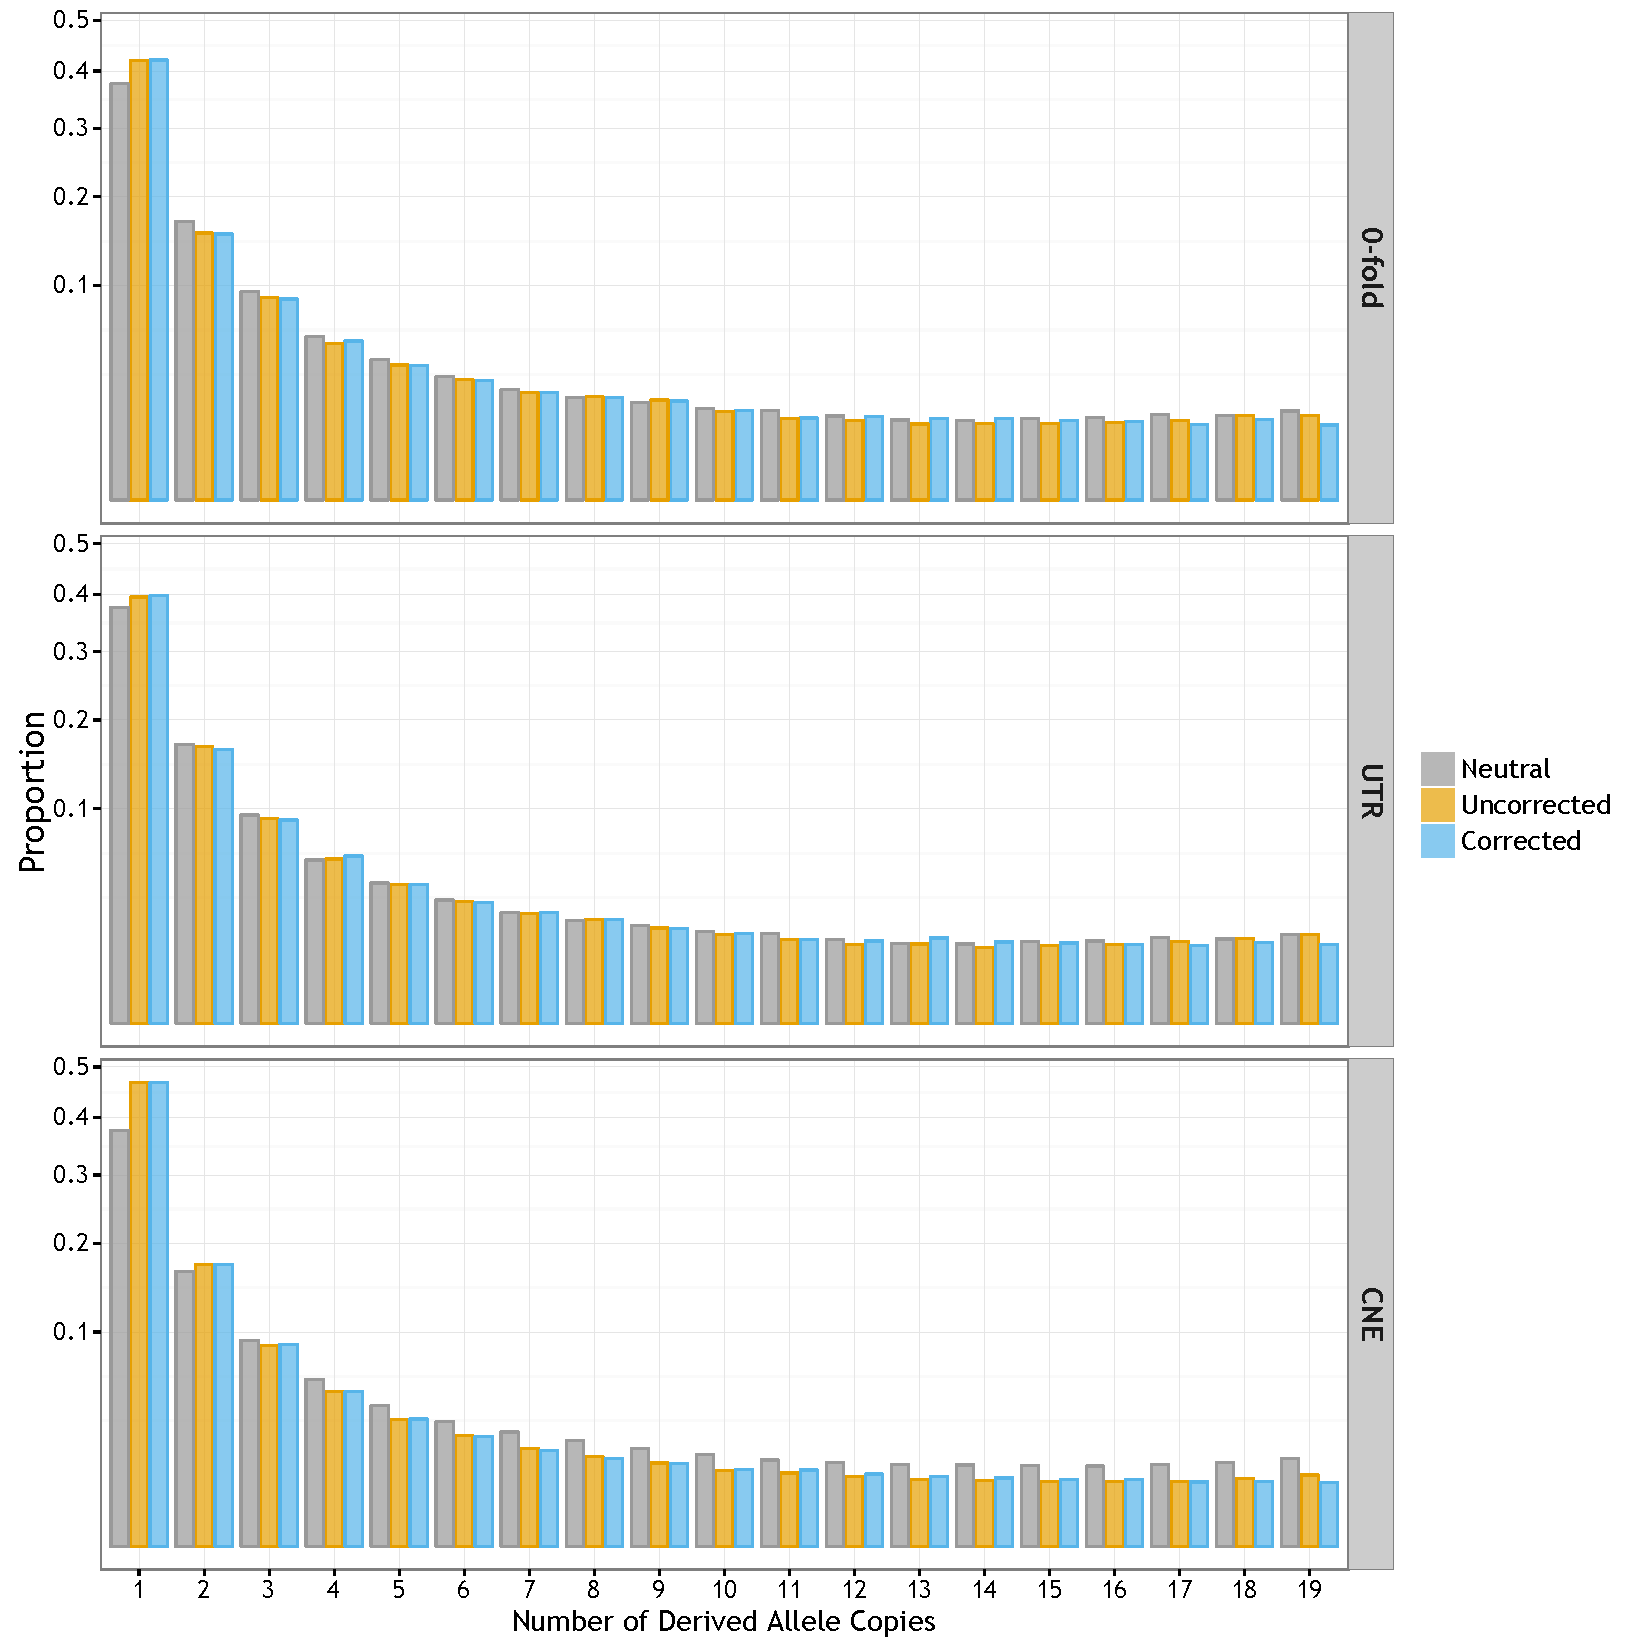
\includegraphics[width=\textwidth]{/Users/s0784966/Dropbox/Thesis/chapter3/Figures/uSFS_raw_comparison.pdf}}
 \caption[The uSFS for multiple classes of sites in the \textit{M. m. castaneus} genome]{The uSFS for three classes of functional sites (yellow and blue bars) compared to a putatively neutral comparator (grey bars). The neutral comparator for 0-fold sites and UTRs was 4-fold degenerate synonymous sites in both cases. For CNEs, the neutral comparator was CNE-flanking sequence. The expected uSFS under a demographic model fitted to a neutral comparator was used to correct the uSFS for the corresponding selected sites (see Methods).}
 \label{fig:uSFS_data}
\end{figure}


\subsection{Estimating the frequencies and strengths of deleterious and advantageous mutations}

	We estimated the DFE for harmful mutations (dDFE) and the rate and strength of advantageous mutations based on the uSFSs for the three different classes of functional sites using DFE-alpha under two different models (Table \ref{tab:DFEestimates}). The first, as described by \cite{RN210}, used the full uSFS, including sites fixed for the derived allele (hereafter Model A). The second (hereafter Model B), incorporated an additional parameter that absorbs the contribution of sites fixed for the derived allele (see Supplementary Methods). This was motivated by the possibility that between-species divergence may be decoupled from within-species polymorphism (e.g. due to changing selection regimes), and this could lead to spurious estimates of selection parameters \cite{RN165, RN354}. Since Model A is nested within Model B, the two can be compared using likelihood ratio tests. In the remainder of the study, results obtained under Model A are shown in parallel with results obtained under Model B. 

\linespread{1}
%\captionsetup{font=script, labelfont=bf , textfont=it}
\begin{table}[h]



 \begin{tabular}{c c c c } \\[ 0.5ex ]
 \hline 
& \multicolumn{2}{c}{Correlation Coefficient}\\ [0.5ex] \cline{2-3}
& Non-CpG Prone Sites & All Sites\\
\hline
Nucleotide diversity ($\pi$) & 0.090 & 0.20 \\
Divergence from rat ($d_{rat}$) & -0.038 & 0.062 \\
Corrected diversity ($\pi/d_{rat}$) & 0.10 & 0.18 \\
\hline

\end{tabular}
\caption[Correlations between recombination rate and genetic diversity]{Correlation coefficients between recombination rate and pairwise nucleotide diversity and divergence from the rat at fourfold degenerate sites for protein coding genes}
\end{table}

\linespread{2}

	We performed a comparison of different DFE models, including discrete distributions with one, two or three mutational effect classes and the gamma distribution including or not including advantageous mutations. For each class of functional sites, DFE models with several classes of deleterious mutational effects and a single class of advantageous effects gave the best fit (Table \ref{tab:C3S4}). For each class of functional sites, only a single class of advantageous mutations was supported, since additional classes of advantageous mutations did not significantly increase likelihoods (Table \ref{tab:C3S5}), presumably reflecting a lack of power. These best-fitting models were identified under both Model A or Model B. Parameter estimates pertaining to the dDFE were also similar between Models A and B (Table \ref{tab:DFEestimates}). 

	In this study, we estimated selection parameters based on the uSFS, whereas earlier studies on mice used the distribution of minor allele frequencies, i.e. the ‘folded’ SFS \citep{RN158, RN170, RN342, RN122, RN238}. A possible consequence of using the folded SFS is that advantageous mutations segregating at intermediate to high frequencies are allocated to the mildly deleterious class. In the case of 0-fold sites, for example, the best-fitting DFE did not include mutations with scaled effects in the range of 1 $<$ $\mid$ $2N_es$ $\mid$ $<$ 200 (Table \ref{tab:DFEestimates}). This contrasts with previous studies using the folded SFS, which identified an appreciable proportion of mutations in the 1 $<$ $\mid$ $2N_es$ $\mid$ $<$ 200 range \citep{RN122,RN178}. This difference may influence the reductions in diversity caused by background selection, so we performed simulations incorporating either the gamma dDFEs inferred from analysis of the folded SFS by \cite{RN122} or the discrete dDFEs inferred in the present study.
 
	For all classes of functional sites, we inferred that moderately positively selected mutations are fairly frequent under both Models A and B (Table \ref{tab:DFEestimates}). In the case of 0-fold sites, for example, the frequency of advantageous mutations was 0.3\% (under Model A). Across the three classes of sites, the scaled selection strengths of advantageous mutations were fairly similar (Table \ref{tab:DFEestimates}), i.e. $2N_es$ ~ 16, implying that $s$ is on the order of $10^{-5}$ (assuming $N_e$ = 500,000; \cite{RN315}). However, we found that estimates of the frequency of advantageous mutations ($p_a$) obtained under Model B for 0-fold sites and UTRs were ~ 3 times higher than those obtained under Model A. In the cases of both 0-fold sites and UTRs, Model B fitted significantly better than Model A, as judged by likelihood ratio tests (0-fold sites, $\chi^{2}_{1 d.f.} = 4.2$; $p$ = 0.04; UTRs, $\chi^{2}_{1 d.f.}= 9.9$; $p$ = 0.002). Interestingly, in the case of CNEs, Models A and B did not differ significantly in fit ($\chi^{2}_{1 d.f.} = 0.26$; $p$ = 0.60) and estimates of the advantageous mutation parameters were similar (Table \ref{tab:DFEestimates}). 

\subsection{Forward-in-time population genetic simulations}

        	We conducted forward-in-time simulations to examine whether estimates of the DFE obtained by analysis of the uSFS predict patterns of diversity observed around functional elements. In our simulations, we used estimates of selection parameters obtained by DFE-alpha for 0-fold sites, UTRs and CNEs assuming either Model A (i.e. from the full uSFS) or Model B (i.e. by absorbing the contribution of sites fixed for the derived allele with an additional parameter). The selection parameter estimates obtained under Models A and B resulted in major differences in the patterns of diversity around functional elements.

\subsubsection{i) Patterns of nucleotide diversity around functional elements in simulated populations}

	Using the selection parameter estimates obtained from DFE-alpha (Table \ref{tab:DFEestimates}), we performed simulations incorporating deleterious mutations, advantageous mutations or both advantageous and deleterious. Our analysis involved computing diversity in windows surrounding functional elements and comparing the diversity patterns with those seen in \textit{M. m. castaneus}. In order to aid visual comparisons, we divided nucleotide diversity ($\pi$) at all positions by the mean π at physical distances greater than 75Kbp and 4Kbp away from exons and CNEs, respectively. When comparisons were made on the scale of genetic distance, we divided $\pi$ by its mean at distances greater than $4N_er$ = 1,500 for protein-coding exons and $4N_er$ = 200 for CNEs. These distances were chosen because they are the values beyond which $\pi$ remains approximately constant. 

	In our simulations, we scaled recombination, mutation and selection parameters by N in a linear fashion. However, linear scaling can become problematic when selection coefficients are strong \citep{RN198}. To test whether linear scaling was appropriate for the parameters we estimated, we simulated populations with N = 100, 500, 750, 1,000 and 2,000. We found that patterns of genetic diversity converged in populations with $N$ = 750, 1,000 and 2,000 (Figure \ref{fig:C3S2}). The following simulations results were obtained assuming $N$ = 1,000. 


	Simulations incorporating only deleterious mutations predicted a chromosome-wide reduction in genetic diversity. Around exons and CNEs, diversity plateaued at ~94\% of the neutral expectation (Figure \ref{fig:C3S3}-\ref{fig:C3S4}). Simulations involving only BGS did not fully predict the observed troughs in diversity around functional elements. Specifically, the predicted troughs in diversity around both protein-coding exons and CNEs, were not as wide nor as deep as those observed in the real data (Figures \ref{fig:piRef_physical}-\ref{fig:piRef_genetic}; \ref{fig:C3S3}-\ref{fig:C3S4}). Similar predictions were obtained for Models A or B (Figures \ref{fig:piRef_physical}-\ref{fig:piRef_genetic}; \ref{fig:C3S3}-\ref{fig:C3S4}) and for the gamma dDFEs inferred by \cite{RN122} (Figure \ref{fig:C3S5}). Our simulations incorporating deleterious mutations suggest, then, that while BGS affects overall genetic diversity across much of the genome, positive selection presumably also makes a substantial contribution to the dips in diversity around functional elements.
	
 \begin{figure}[H]
   \centering      
   \noindent\makebox[\textwidth]{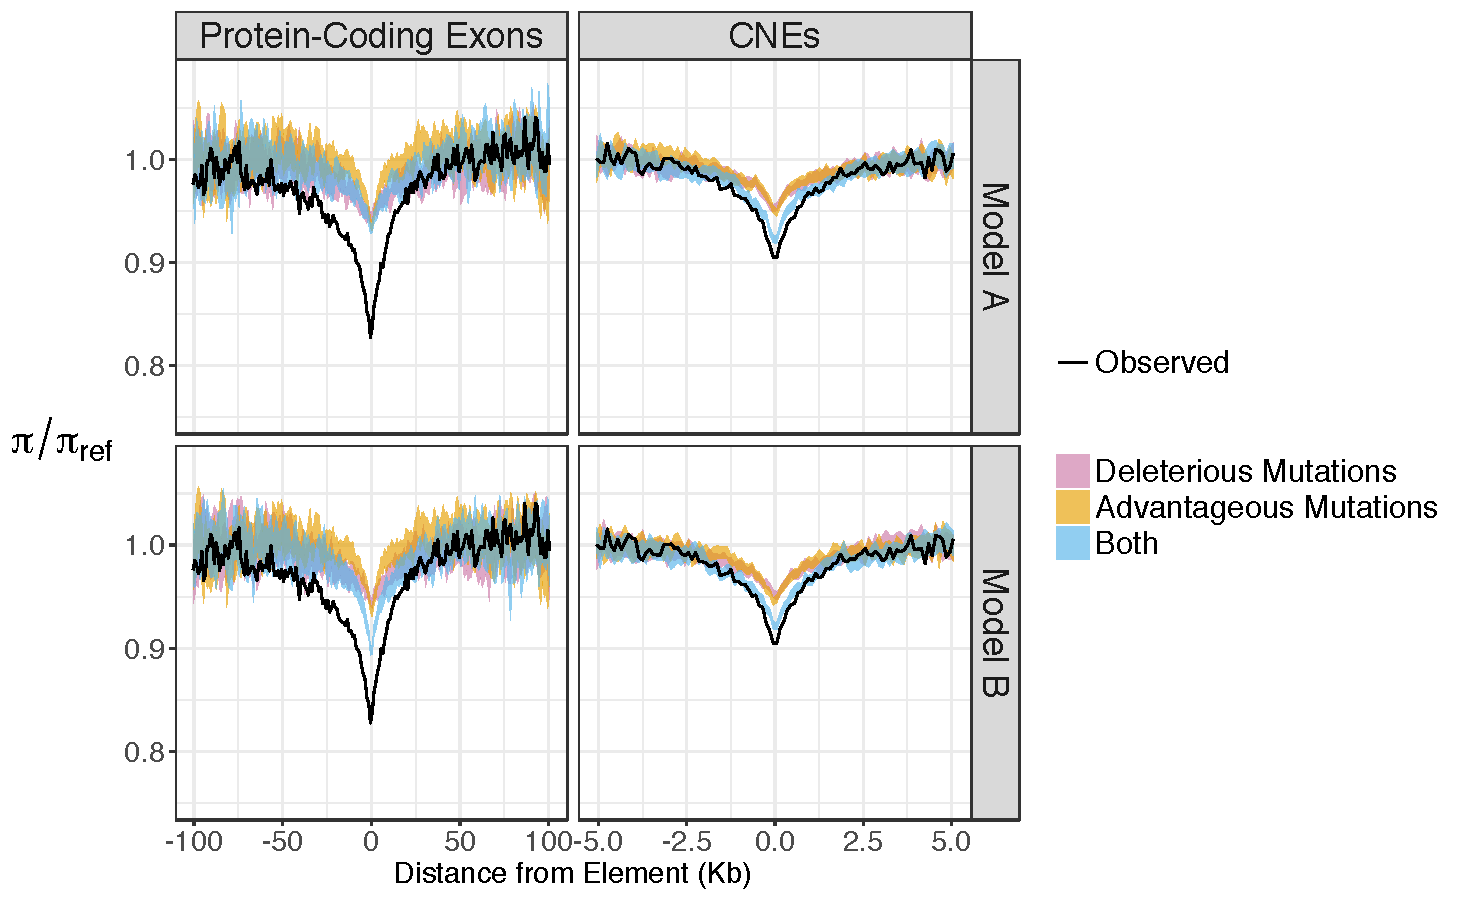
\includegraphics[width=\textwidth]{/Users/s0784966/Dropbox/Thesis/chapter3/Figures/Pi_ref_2x2.pdf}}
 \caption[Reductions in diversity caused by background selection and selective sweeps in simulated data - physical distance]{Estimates of scaled diversity ($\pi / \pi_{Ref}$) around protein-coding exons and CNEs (black lines) in \textit{M. m. castaneus} compared to results from simulations (colored ribbons). The panels show diversity observed in simulated populations assuming DFE estimates obtained by analysis of the full uSFS (Model A) or when sites fixed for the derived allele do not influence selection parameters (Model B). Colored ribbons represent 95\% confidence intervals obtained from 1,000 bootstrap samples.}
 \label{fig:piRef_physical}
\end{figure}

 \begin{figure}[H]
   \centering      
   \noindent\makebox[\textwidth]{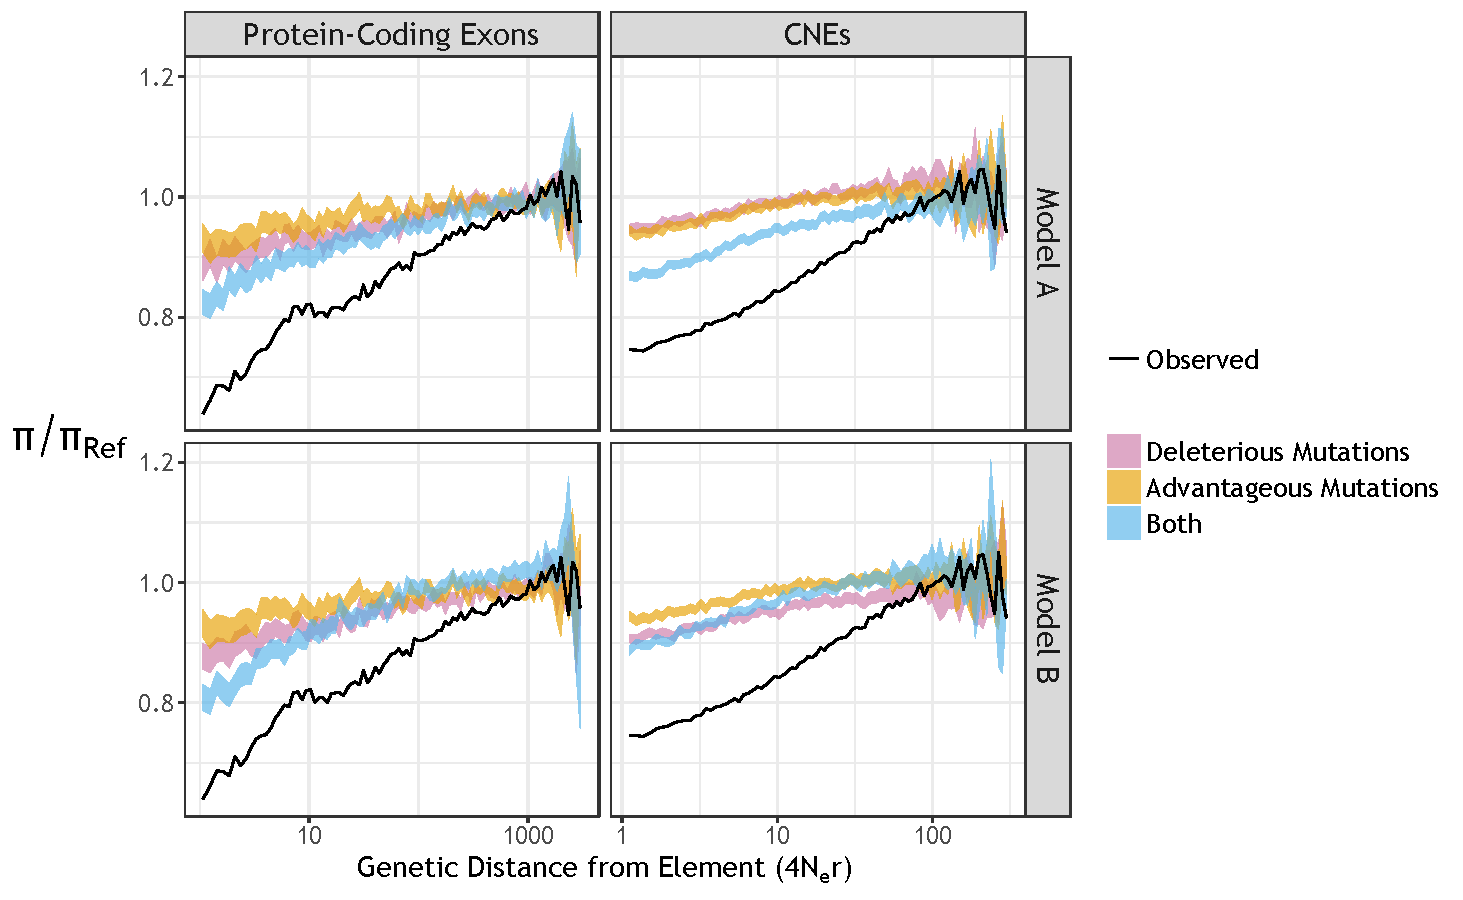
\includegraphics[width=\textwidth]{/Users/s0784966/Dropbox/Thesis/chapter3/Figures/Pi_ref_Genetic_2x2.pdf}}
 \caption[Reductions in diversity caused by background selection and selective sweeps in simulated data - genetic distance]{Estimates of scaled diversity ($\pi / \pi_{Ref}$) plotted against genetic distance from exons and conserved non-coding elements (CNEs) in \textit{M. m. castaneus} compared to results from simulations (colored ribbons). The panels show diversity observed in simulated populations assuming DFE estimates obtained by analysis of the full uSFS (Model A) or when sites fixed for the derived allele do not influence selection parameters (Model B). Nucleotide diversity ($\pi$) is scaled by the mean diversity at population-scaled genetic distances ($4N_er$) more than 1,500 from exons and 200 from CNEs ($\pi_{Ref}$). Colored ribbons represent 95\% confidence intervals obtained from 1,000 bootstrap samples. Diversity downstream of functional elements is shown.}
 \label{fig:piRef_genetic}
\end{figure}

	In our simulations of exons and surrounding regions, recurrent SSWs produced troughs in diversity, but they were both narrower and shallower than those observed in the house mouse. However, the results are sensitive to the model used to estimate selection parameters (Figure \ref{fig:piRef_physical}; Table \ref{tab:RMS}). Assuming the selection parameters estimated under Model A (i.e. analysing the full uSFS) we found that advantageous mutations produced a small dip in diversity around exons, which was both shallower and narrower than the one generated by deleterious mutations alone (Figure \ref{fig:piRef_physical}; Table \ref{tab:RMS}). In contrast, the advantageous mutation parameters estimated under Model B (i.e. where sites fixed for the derived allele do not influence selection parameters) resulted in a marked trough in diversity around exons in simulations (Figure \ref{fig:piRef_physical}; Table \ref{tab:RMS}). In simulations incorporating both advantageous and deleterious mutations, the troughs in diversity around exons were not as large as those observed in\textit{M. m. castaneus} (Figure \ref{fig:piRef_physical}; Table \ref{tab:RMS}), and even at very large distances from exons, diversity was around 90\% of neutral expectation (Figure \ref{fig:C3S3}). Assuming Model B selection parameters resulted in a trough in diversity that was both deeper and wider than the one generated when assuming Model A parameters (Figure \ref{fig:piRef_physical}). The differences between Model A simulations and Model B simulations presumably arise because under Model B the frequency of advantageous nonsynonymous mutations was ~3 times higher than under Model A (Table \ref{tab:DFEestimates}). When analysis windows are binned based on genetic distance rather than physical distance, the differences between observed and simulated diversity patterns are even more striking (Figure \ref{fig:piRef_genetic} and Figure \ref{fig:C3S4}). 


	We also carried out simulations focussing on CNEs and found that the combined effects of BGS and recurrent SSWs, as generated by our estimates of selection parameters, resulted in diversity troughs that were slightly shallower than observed (Figure \ref{fig:piRef_physical}; Table \ref{tab:RMS}). Selection parameters obtained under Models A and B produced similar results. The troughs in diversity around CNEs in simulations incorporating only advantageous mutations were slightly shallower than the ones generated by deleterious mutations alone (Figure \ref{fig:C3S4}). The troughs in diversity around CNEs in our simulations were also slightly shallower than those observed (Figure \ref{fig:piRef_physical}). This could be because we failed to detect infrequent, strongly selected advantageous mutations in CNEs or we underestimated the true frequency of advantageous mutations occurring in those elements. When plotted on the scale of genetic distance, the differences between our simulated data and the \textit{M. m. castaneus} data become strikingly apparent (Figure \ref{fig:piRef_genetic}). 


\subsubsection{ii) The site frequency spectrum around functional elements}

	SSWs and BGS are known to affect the shape of the SFS for linked neutral sites \citep{RN287, RN234, RN343}. SSWs and BGS generate troughs in diversity at linked sites (Figures \ref{fig:piRef_physical} and \ref{fig:piRef_genetic}), but nucleotide diversity on its own does not contain information about the shape of the SFS. Tajima’s $D$ is a useful statistic for this purpose, because it is reduced when there is an excess of rare polymorphisms relative to the neutral expectation and increased when intermediate frequency variants are more common \citep{RN90}. We therefore compared Tajima’s $D$ in the regions surrounding functional elements in simulations with values observed in the real data. It is notable that average Tajima’s $D$ is far lower in \textit{M. m. castaneus} than in our simulations (Figure \ref{fig:TajimaPlot}). This likely reflects a genome-wide process, such as population size change, that we have not modelled.

 \begin{figure}[H]
   \centering      
   \noindent\makebox[\textwidth]{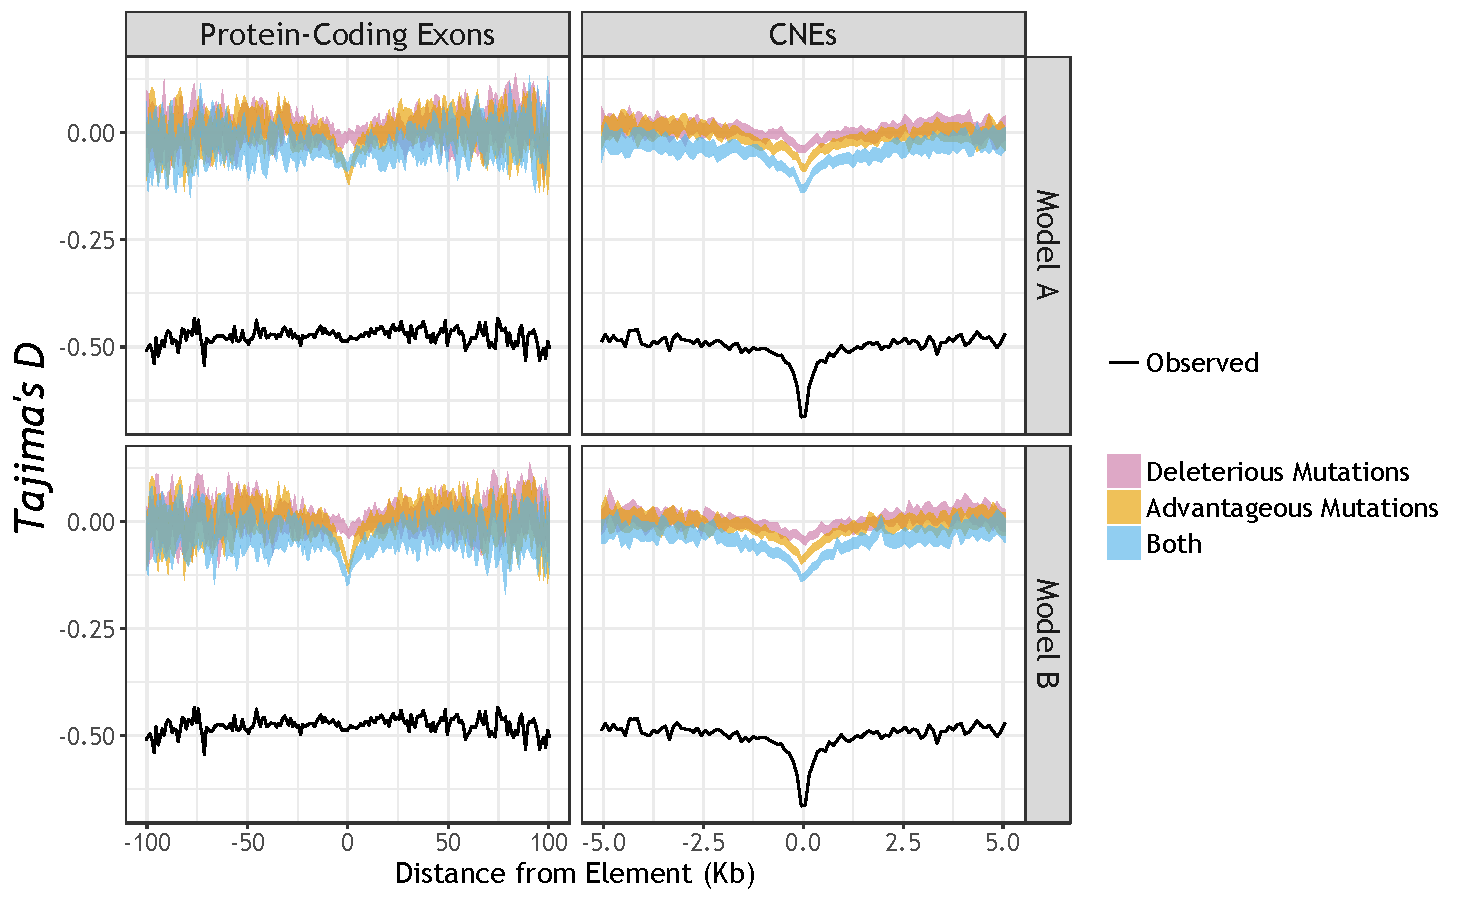
\includegraphics[width=\textwidth]{/Users/s0784966/Dropbox/Thesis/chapter3/Figures/Tajima_ExonCNE.pdf}}
 \caption[Tajima's $D$ around functional elements in \textit{M. m. castaneus} and simulated populations]{Tajima’s $D$ around protein-coding exons and CNEs in \textit{M. m. castaneus} compared to simulated data. The black lines show Tajima’s $D$ computed from the \textit{M. m. castaneus} genome sequence data around protein-coding exons or CNEs. The coloured ribbons show the 95\% bootstrap intervals from simulated data assuming the DFEs estimated under either Model A (i.e. analysing the full uSFS) or Model B (i.e. fixed derived sites do not contribute to the likelihood for selection parameters)}
 \label{fig:TajimaPlot}
\end{figure}


	If we assume selection parameters obtained under Model A, Tajima’s $D$ around protein-coding exons is relatively invariant, and matches the pattern observed in the real data fairly well (Figure \ref{fig:TajimaPlot}). However, under Model B, the simulations exhibit a marked dip in Tajima’s $D$, which is not observed in the real data (Figure \ref{fig:TajimaPlot}).

	In the case of CNEs, we observed a trough in Tajima’s $D$ in the real data (Figure \ref{fig:TajimaPlot}), and simulations predict similar troughs under Models A and B (Figure 4). However, the trough in Tajima’s $D$ may be caused by the presence of functionally constrained sequences in the immediate flanks of CNEs (See Methods), making a comparison between the simulations and the observed data problematic.

\subsubsection{iii) Rates of substitution in functional elements}

Incorporating information from sites fixed for the derived allele when estimating the DFE (as in Model A) or disregarding this information (as in Model B) had a striking effect on estimates of the frequency and effects of advantageous mutations (Table \ref{tab:DFEestimates}). In the case of 0-fold sites, for example, $p_a$ was ~3x higher under Model B than Model A (Table \ref{tab:DFEestimates}). We therefore investigated the extent by which such differences affect the divergence at selected sites under the two models. Nucleotide divergence at putatively neutral sites between the mouse and the rat is approximately 15\%, so we simulated an expected neutral divergence of 7.5\% for one lineage. 

We compared the ratio of nucleotide divergence at selected sites to the divergence at neutral sites ($d_[sel]/d_[neut]$) between the simulated and observed data. In simulations that assumed the selection parameters obtained under Model A, $d_{sel}/d_{neut}$ values were similar to those observed in \textit{M. m. castaneus} for all classes of selected sites (Table \ref{tab:Divergence}). Under Model B, however, the simulations predicted substantially more substitutions at nonsynonymous sites and UTRs than were seen in the real data (Table \ref{tab:Divergence}). This suggests that, under Model B, the frequency of advantageous mutations for 0-fold sites and UTRs may be overestimated.

\subsubsection{iv) Examining the uSFS and estimating the DFE from simulated data}

	BGS and SSWs both perturb allele frequencies at linked neutral sites, distorting site frequency spectra, which can lead to the inference of spurious demographic histories \citep{RN149, RN241, RN242}. By fitting a model incorporating three epochs of population size to the putatively neutral site data, we inferred that \textit{M. m. castaneus} has experienced a population bottleneck followed by an expansion (Table \ref{tab:C3S2}). To investigate the possibility that the inferred demographic histories could be an artefact of selection at linked sites, we fitted demographic models to the uSFS obtained from simulated synonymous sites. Visual comparison of the uSFS from simulated populations with the uSFS obtained from \textit{M. m. castaneus} reveals that our simulations do not fully capture the excess of high frequency variants observed in the mouse population (Figure \ref{fig:C3S6}). However, for simulations assuming the selection parameters obtained under either Model A or B, a 3-epoch population size model gave the best fit to the data. The estimated demographic histories were somewhat different between simulations assuming Model A or Model B, but in each case a population bottleneck followed by an expansion was inferred (Table \ref{tab:C3S6}). This is an interesting observation: our simulations assumed a constant population size, but selection at linked sites appears to distort the neutral uSFS, such that a demographic history similar to the one inferred from the real data is estimated (Table \ref{tab:C3S6}).  

	Our simulations also indicate that selection parameters are difficult to accurately infer using the uSFS alone. In the case of Model A simulations, the selection strength and frequency of deleterious mutations was accurately estimated, as was the combined frequency of all effectively neutral mutations (Table \ref{tab:C3S6}). However, in Model A simulations, DFE-alpha did not accurately estimate the strength and frequency of advantageous mutations. Estimates of selection parameters in Model B simulations were similar to the input parameters, but a notable exception was that the frequency of advantageous mutations ($p_a$) was overestimated (Table \ref{tab:C3S6}). These results suggest that some features of the uSFS inferred for \textit{M. m. castaneus} have been captured by our simulated data. However, the demographic correction which we applied to the uSFS before estimating selection parameters (see Supplementary Methods), had a substantially greater impact on the \textit{M. m. castaneus} data than for the simulated data, particularly in the case of high frequency derived alleles (Figure \ref{fig:C3S6}). A possible explanation is that strong SSWs, which cause a greater increase in the proportions of high frequency derived alleles for linked sites \citep{RN343}, have left a signal in the neutral site uSFS, but these cannot be accurately inferred from the selected site uSFS itself. If this were the case, then there may be information in the uSFS for linked neutrally evolving sites that could be used when estimating selection parameters. This would require the expected uSFS arising under the joint effects of SSWs and BGS.

\linespread{1}
\begin{table}[H]
\centering
\caption[The root mean square difference between values of $\pi$ around functional elements predicted in simulations and $\pi$ observed in \textit{M. m. castaneus}.]{The root mean square difference between values of $\pi$ around functional elements predicted in simulations and $\pi$ observed in \textit{M. m. castaneus}. Confidence intervals were obtained from 1,000 bootstrap samples (see Methods). Values shown are for the patterns of diversity when measured on the scale of physical distance.}
\begin{adjustbox}{max width=\textwidth}

\begin{tabular}{cccccc}
\toprule
           &                &         \multicolumn{2}{c}{Exons} &         \multicolumn{2}{c}{CNEs}  \\

           &                         &  Median &        95\% range &  Median &        95\% range \\ \midrule
   \multirow{3}{*}{Model A} &   Deleterious Mutations &  0.0327 &  0.0311 - 0.0343 &  0.0164 &  0.0151 - 0.0179 \\
        &  Advantageous Mutations &  0.0422 &  0.0403 - 0.0442 &  0.0177 &  0.0161 - 0.0195 \\
        &                    Both &  0.0312 &  0.0297 - 0.0340 &    0.01 &  0.0088 - 0.0113 \\ \hdashline
   \multirow{3}{*}{Model B} &   Deleterious Mutations &  0.0331 &  0.0314 - 0.0351 &  0.0157 &  0.0144 - 0.0171 \\
        &  Advantageous Mutations &   0.038 &  0.0355 - 0.0406 &  0.0162 &  0.0147 - 0.0179 \\
        &                    Both &  0.0274 &  0.0253 - 0.0294 &  0.0088 &  0.0078 - 0.0101 \\
\bottomrule
\end{tabular}
\end{adjustbox}
\label{tab:RMS}
\end{table}
\linespread{2}


\subsubsection{v) Patterns of diversity around sites that have recently experienced a substitution}

	In general, it has been difficult to discriminate between BGS and SSWs, because their effects on genetic diversity and the site frequency spectrum are qualitatively similar. It has been suggested that the two processes can be teased apart by taking advantage of the fact that hard SSWs should be centred on a nucleotide substitution, whereas this is not the case for BGS. Comparing the average genetic diversity in regions surrounding recent putatively selected and putatively neutral substitutions (e.g. 0-fold and 4-fold sites, respectively) may therefore reveal the action of SSWs \citep{RN162, RN167}. \cite{RN122} performed such an analysis in \textit{M. m. castaneus} using the closely related \textit{M. famulus} as an outgroup, and found that the profiles of neutral diversity around 0-fold and 4-fold substitutions were virtually identical. Similar findings have been reported in other species \citep{RN162,RN230}. One interpretation of these results is that hard SSWs are rare. To investigate this, we measured the average neutral diversity around nonsynonymous and synonymous substitutions in simulations for the case of frequent hard SSWs.


 \begin{figure}[H]
   \centering      
   \noindent\makebox[\textwidth]{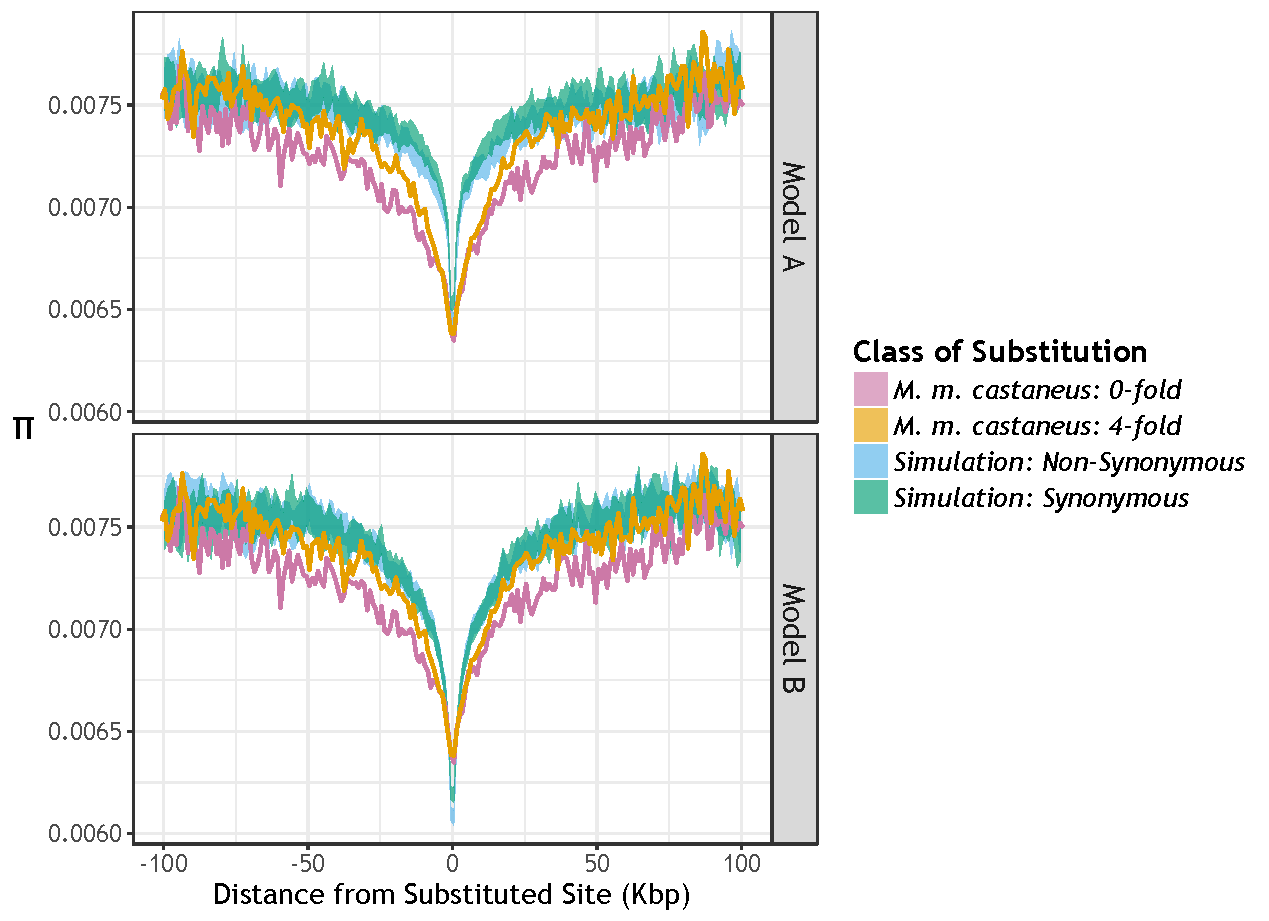
\includegraphics[width=\textwidth]{/Users/s0784966/Dropbox/Thesis/chapter3/Figures/SubstitutionPlot.pdf}}
 \caption[Reductions in nucleotide diversity around recent substitutions in \textit{M. m. castaneus} and simulated populations]{Nucleotide diversity ($\pi$) around substituted sites in \textit{M. m. castaneus} compared to the same pattern obtained from simulation data. Nucleotide diversity in \textit{M. m. castaneus} was scaled by divergence between mouse and rat to correct for variation in local mutation rates. The \textit{M. m. castaneus} data are from \cite{RN122}. }
 \label{fig:SattathPlot}
\end{figure}


	In our simulations, we measured diversity around substitutions occurring on a time-scale equivalent to the divergence time between \textit{M. m. castaneus} and \textit{M. famulus}. The average diversities around nonsynonymous and synonymous substitutions in the simulated data were very similar, regardless of whether simulations assumed Model A or Model B selection parameters (Figure \ref{fig:SattathPlot}). However, the troughs in diversity around substitutions were deeper in the simulations assuming Model B (Figure \ref{fig:SattathPlot}), reflecting the higher frequency of advantageous mutations (Table \ref{tab:DFEestimates}). In the immediate vicinity of nonsynonymous substitutions, diversity was lower than the corresponding value for synonymous substitutions (Figure \ref{fig:SattathPlot}). However, the differences are slight, so it would be difficult to draw firm conclusions about the action of either SSWs or BGS. Taken together, these results suggest that analysing patterns of diversity around recent substitutions does not provide enough information to convincingly discriminate between SSWs and BGS in \textit{M. m. castaneus}, even when hard sweeps are fairly frequent. Further analysis is required to assess whether this is also the case for other organisms.

\linespread{1}
\begin{table}[H]
\centering
\caption[Accumulation of divergence in simulated populations]{Comparison of the accumulation of nucleotide divergence in simulated populations between different functional site types. In the cases of 0-fold sites and UTRs, $d_{neu}$ refers to 4-fold sites. For CNEs, $d_{neu}$ refers to CNE flanking sites. In all simulations, $d_{neu}$ was set to 7.5\%.}

\begin{tabular}{cccccc}
\toprule
            & 							& \multicolumn{4}{c}{Simulation DFE}\\
            &  \textit{M. m. castaneus} &        \multicolumn{2}{c}{Model A}             &    \multicolumn{2}{c}{Model B} \\ \hdashline
 Site Class &       $d_{sel}$/$d_{neu}$ &          $d$ (\%) &  $d_{sel}$/$d_{neu}$ &      d (\%) &  $d_{sel}$/$d_{neu}$ \\ \midrule
     0-fold &           0.225           &           1.66 &      0.221 &       2.26 &      0.301 \\
        UTR &           0.757           &           5.76 &      0.767 &       6.85 &      0.914 \\
        CNE &           0.406           &           3.31 &       0.44 &       3.07 &      0.409 \\
\bottomrule
\end{tabular}
\label{tab:Divergence}
\end{table}
\linespread{2}

\section{Discussion}

There are a number of observations suggesting that natural selection is pervasive in the murid genome. First, there is a positive correlation between synonymous site diversity and the rate of recombination \citep{RN340}. Secondly, there is reduced diversity on the X-chromosome compared to the autosomes, which cannot readily be explained by neutral or demographic processes \citep{RN233}. Thirdly, there are troughs in genetic diversity surrounding functional elements, such as protein-coding exons and CNEs, which are consistent with the action of BGS and/or SSWs \citep{RN122}. In this paper, we analysed the sequences of 10 \textit{M. m. castaneus} individuals sampled from the ancestral range of the species \citep{RN122}. We estimated the DFEs for several classes of functional sites (0-fold nonsynonymous sites, UTRs and CNEs), and used these estimates to parametrise forward-in-time simulations. We investigated whether the simulations predict the observed troughs in diversity around functional elements along with the between-species divergence observed between mice and rats.

\subsection{Estimating selection parameters based on the uSFS}

	Relative to putatively neutral comparators, 0-fold sites, UTRs and CNEs all exhibited reduced nucleotide diversity, reduced nucleotide divergence and an excess of low frequency variants (Table \ref{tab:CastSummaryStats}; Figure \ref{fig:uSFS_data}), consistent with the action of natural selection \citep{RN158, RN122}. The estimates of the DFEs included substantial proportions of strongly deleterious mutations (Table \ref{tab:DFEestimates}). In addition, the best-fitting models also included a single class of advantageous mutations. Although additional classes were not statistically supported, in reality, there is almost certainly a distribution of advantageous selection coefficients \citep{RN181, RN345}. A visual examination of the fitted and observed uSFSs, however, shows that the estimated DFEs fitted the data very well (Figure \ref{fig:C3S7}), suggesting that there is limited information in the uSFS to estimate a range of positive selection coefficients. 

	When estimating the DFE for a particular class of sites, we analysed either the full uSFS including sites fixed for the derived allele (Model A) or we ignored sites fixed for the derived allele (i.e. Model B). Recently,\cite{RN354} showed that selection parameters can be accurately estimated from the uSFS in simulations that ignored between-species divergence, if the frequency of advantageous mutations ($p_a$) is sufficiently high. In our analysis of 0-fold sites and UTRs, Model B gave a significantly better fit and higher estimates pa than Model A (Table \ref{tab:DFEestimates}). For CNEs, however, Models A and B did not significantly differ in fit, and the selection parameter estimates were very similar (Table \ref{tab:DFEestimates}). The goodness-of-fit and parameter estimates obtained under Models A and B may differ if the processes that generated between species-divergence are decoupled from the processes that produce within species diversity. There are several factors that could potentially cause such a decoupling. 1) Past demographic processes may have distorted the uSFS in ways not captured by the corrections we applied; 2) there may be error in assigning alleles as ancestral or derived; 3) the nature of the DFE may have changed since the accumulation of between-species differences began; and 4) there could be rare, strongly advantageous mutations that contribute to divergence, but contribute negligibly to polymorphism. It is difficult to know which of these factors affected the outcome of our analyses. However, we found that Model B gave a better fit to the uSFS than Model A for 0-fold sites and UTRs, but not CNEs. There is an a priori expectation that the strength of selection on protein-coding sequences is greater than regulatory sequences \cite{RN122}, so we think the latter factor is likely to have been important. 

\subsection{Patterns of diversity and Tajima’s D around functional elements}

	We performed simulations incorporating our estimates of deleterious and advantageous mutation parameters to dissect the contribution of BGS and selective sweeps to diversity dips around functional elements. Our simulations suggest that BGS and SSWs both produce genome-wide reductions in neutral diversity (Figures \ref{fig:C3S3}-\ref{fig:C3S4}), but neither process on its own fully explains the troughs in diversity around protein-coding exons and CNEs, regardless of which model (A or B) is used to estimate selection parameters (Figures \ref{fig:piRef_physical}-\ref{fig:piRef_genetic}). Around protein-coding exons, the combined effects of advantageous and deleterious mutations generated a shallower trough in diversity than the one observed (Figure \ref{fig:piRef_physical}). These patterns are qualitatively similar when analysing physical or genetic distances, but the differences between observed and simulated patterns are more apparent when analysing genetic distances (Figure \ref{fig:piRef_genetic}). A possible explanation for this is that rare, strongly selected advantageous mutations are undetectable by analyses based on the uSFS (discussed below). In contrast, the combined effects of BGS and SSWs predicted troughs in diversity surrounding CNEs that closely match those observed, when measured on the physical scale (Figure \ref{fig:piRef_physical}). Troughs of diversity around CNEs on the scale of genetic distance are not nearly so similar in simulated populations to those observed in \textit{M. m. castaneus} as they are on the physical scale. Specifically, the observed trough in diversity around CNEs on the genetic distance scale is both deeper and wider than in simulated populations. Analysing patterns of diversity on the physical scale is analogous to assuming that there is a uniform recombination rate across the genome. Our results highlight the importance of incorporating recombination rate variation when performing such analyses, particularly in species that exhibit highly variable recombination rates.

	There is an excess of rare variants in \textit{M. m. castaneus} relative to the neutral expectation, as indicated by a strongly negative Tajima’s $D$s for putatively neutral sites (Table 1) and for regions surrounding exons and CNEs (Figure \ref{fig:TajimaPlot}). Our simulations incorporating both advantageous and deleterious mutations also exhibited negative Tajima’s $D$, but not nearly so negative as in the real data (Figure \ref{fig:TajimaPlot}). This difference between the observed data and the simulations indicates that there may be processes generating an excess of rare variants, such as a recent population expansion, which were not incorporated in the simulations.

\subsection{Rates of nucleotide substitutions in simulations}

	Our simulations suggest that the frequency of advantageous mutations (pa) estimated for 0-fold sites and UTRs under Model B may be unrealistically high. This is because several aspects of the results were incompatible with the observed data. Firstly, we found that the substitution rates for simulated nonsynonymous and UTR sites were higher than those observed between mouse and rat (Table \ref{tab:Divergence}). Secondly, we observed a pronounced dip in Tajima’s $D$ around simulated exons, which is not present in the real data (Figure \ref{fig:TajimaPlot}), suggesting that under Model B, either the strength or frequency of positive selection at 0-fold sites is overestimated. 

\subsection{Do our results provide evidence for strongly selected advantageous mutations?}

	Estimation of the strength and frequency of advantageous mutations based on the uSFS relies on the presence of positively selected variants segregating within the population \citep{RN201, RN210, RN354}. The frequency of advantageous mutations may impose a limit on the parameters of positive selection that can be accurately estimated. Indeed, \cite{RN354} recently showed that $p_a$ may be overestimated when analysing the uSFS, if the true value of $p_a$ is low. 

	If advantageous mutations are infrequent, those with larger effects on fitness will be less likely to observed segregating than those with milder effects, as strongly selected mutations have shorter sojourn times than weakly selected ones \cite{RN400,RN401}. This could explain why the selection parameters we estimated fail to predict the troughs in diversity observed in the real data (Figure \ref{fig:piRef_physical}). Furthermore, the fact that Model B gave a better fit than Model A for 0-fold sites and UTRs suggests that polymorphism and divergence have become decoupled for those sites. This is also consistent with the presence of infrequent, strongly selected mutations that become fixed rapidly and are thus not commonly observed as polymorphisms.

	Relevant to this point, an interesting comparison can be made between two recent studies to estimate the frequency and strength of positive selection using the same \textit{D. melanogaster} dataset. The first, by \cite{RN321}, used the uSFS analysis methods of \cite{RN210} (i.e. Model A in the present study), and estimated the frequency of advantageous mutations ($p_a$) = $4.5 x 10^{-3}$ and the scaled strength of selection ($2N_es_a$) = 23.0 for 0-fold nonsynonymous sites. In the second study,  \cite{RN290} estimated $p_a$ = 2.2 x $10^{-4}$ and $2N_es_a$ = 241, based on the correlation between synonymous site diversity and nonsynonymous site divergence. Although the individual parameter estimates differ substantially, the compound parameter $2N_es_ap_a$ (which approximates the rate of SSWs) was similar between the studies (0.055 and 0.104 for \cite{RN290} and cite{RN321} respectively). It is expected that synonymous site diversity is reduced by SSWs, so the method used by \cite{RN290} may be sensitive to the presence of strongly selected mutations, whereas the \cite{RN321} approach may have been more sensitive to weakly selected ones. It seems plausible then, that the two studies capture different aspects of the DFE for advantageous mutations (a similar argument was made by \citealt{RN171}). Supporting this view, \cite{RN274} recently estimated the DFE in \textit{D. melanogaster}, incorporating both strongly and weakly selected advantageous mutations, by fitting a model incorporating BGS and SSWs to genome-wide variation in genetic diversity. They inferred that weakly selected mutations are far more frequent than strongly selected ones, but that both contribute to variation in genetic diversity across the \textit{D. melanogaster} genome. In the present study, we used similar methods as \cite{RN321} to estimate the frequency and strength of advantageous mutations, so the estimated parameters of positive selection may represent only weakly selected mutations. Indeed, patterns of diversity at microsatellite loci suggest that there are strongly selected, infrequent sweeps in multiple European \textit{M. musculus} populations \citep{RN355}, so infrequent strong sweeps may be a general feature of mouse evolution.

	We tested the hypothesis that undetected, strongly selected mutations are chiefly responsible for the reductions in diversity around functional elements by performing additional simulations. In this exercise, we assumed far stronger selection on advantageous mutations for protein-coding regions than we estimated for 0-fold sites (Table \ref{tab:C3S7}). When modelling strong selection, we reduced pa such that rate of sweeps (proportional to the product $2N_es_ap_a$) was either that estimated from the uSFS under Model A, or double that value (Table \ref{tab:C3S7}). As can be seen in Figure \ref{fig:strongSelection}, increasing the strength of selection acting on advantageous mutations, while simultaneously decreasing the $p_a$ parameter resulted in troughs in diversity around protein-coding exons that were both deeper and wider than those observed in \textit{M. m. castaneus}. By chance, we identified a set of parameters ($2N_es_a$ = 400; $p_a$ = 0002) that can provide a relatively close correspondence between simulated and observed patterns of diversity. However, it must be stressed that these parameters were chosen arbitrarily and that there is no statistical support for them.

\begin{figure}[H]
   \centering      
   \noindent\makebox[\textwidth]{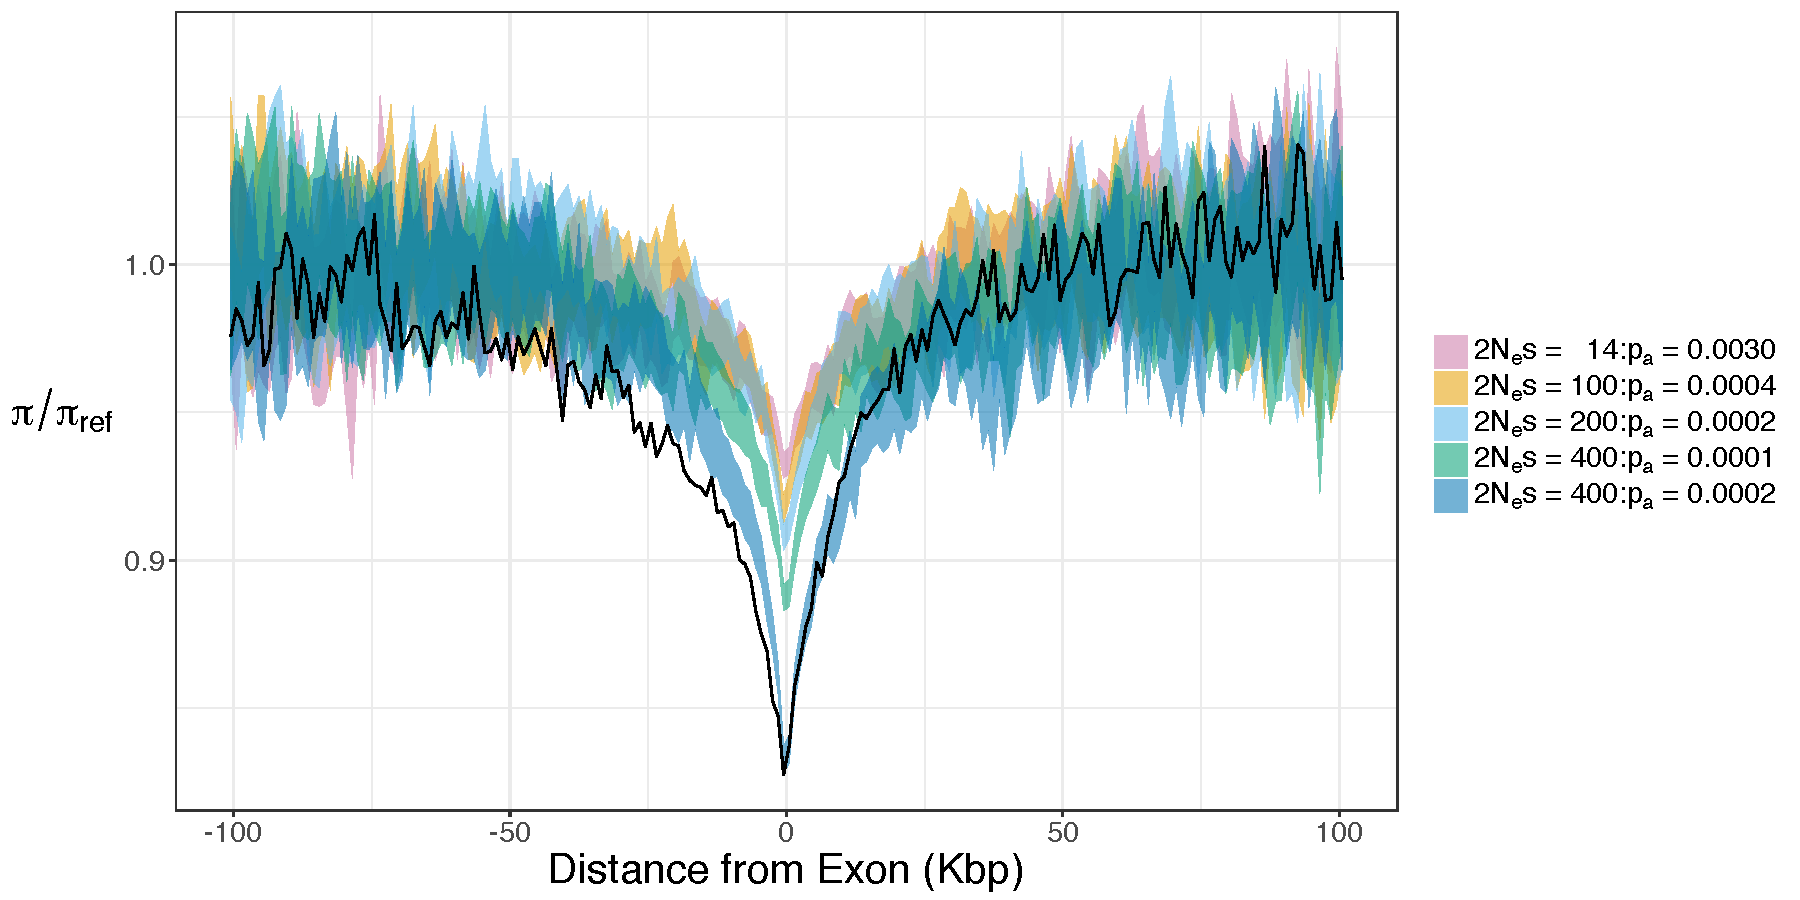
\includegraphics[width=\textwidth]{/Users/s0784966/Dropbox/Thesis/chapter3/Figures/StrongSelectionPiRed.pdf}}
 \caption[Reductions in diversity around exons caused by strong positive selection]{Patterns of nucleotide diversity around protein-coding exons in simulations assuming strongly selected advantageous mutations. Nucleotide diversity in \textit{M. m. castaneus} is shown in black. Nucleotide diversity ($\pi$) is scaled by the mean diversity at distances more than 75 Kbp from exons ($\pi_{Ref}$). Coloured ribbons represent 95\% confidence intervals obtained from 1,000 bootstrap samples.}
 \label{fig:strongSelection}
\end{figure}

	Although strongly selected mutations can generate a similar trough in average diversity around protein-coding exons as observed in the real data, they do not produce the apparent genome-wide reduction in Tajima’s $D$ observed in \textit{M. m. castaneus} (Figure \ref{fig:C3S8}). Indeed, in all simulations modelling strongly advantageous mutations, we observed a trough in Tajima’s $D$ that plateaued at values close to 0 in regions surrounding protein-coding exons (Figure \ref{fig:C3S8}). In this exercise, we manipulated the selection parameters for 0-fold sites only, but it is possible that there are strongly advantageous mutations in all of the site classes. A combination of DFE parameters for the different functional elements in mice could therefore explain the reductions in diversity and the genome-wide negative Tajima’s $D$. On the other hand, it could also be that recent demographic processes have swamped the signal of linked positive selection in the site frequency spectrum.  Our results highlight the need for methods that can simultaneously estimate selection parameters for multiple functional elements and demographic history. 

	Understanding the contributions of regulatory and protein change to phenotypic evolution has been an enduring goal in evolutionary biology \cite{RN347, RN346, RN348}. If selection is strong relative to drift (i.e. $2N_es_a$ > 1) then the rate of change of fitness from the fixation of advantageous mutations is expected to be proportional to the square of the selection coefficient \citep{RN391}. In this study, we inferred that the strength of selection acting on new advantageous mutations in CNEs and 0-fold sites are roughly equivalent, but that advantageous mutations occur more frequently in CNEs (Table \ref{tab:DFEestimates}). Given that there are more CNE nucleotides in the genome than there are 0-fold sites (Table \ref{tab:CastSummaryStats}), this could imply that adaptation at regulatory sites causes the greatest fitness change in mice. However, our analyses suggest that both protein-coding genes and CNEs may experience strongly selected advantageous mutations, which are undetectable by analysis of the uSFS. If this were the case, protein-coding mutations could make a larger contribution to fitness change than mutations in regulatory sites.

\subsection{Limitations of the study}

	There is a growing body of evidence suggesting that hard sweeps may not be the primary mode of adaptation in both \textit{D. melanogaster} and humans. Firstly, soft sweeps, where multiple haplotypes reach fixation due to the presence of multiple de novo mutations or selection acted on standing variation, may be common. \cite{RN208} developed a suite of haplotype-based statistics that can discriminate between soft and hard SSWs. The application of these statistics to North American and Zambian populations of \textit{D. melanogaster} suggested that soft sweeps are the dominant mode of adaptation in that species, at least in recent evolutionary time \citep{RN208,RN303}. Furthermore, \cite{RN337} recently reported that signatures of soft sweeps are more frequent than those of hard sweeps in humans. However, their method did not explicitly include the effects of partial sweeps and/or BGS. Under a model of stabilising selection acting on a polygenic trait, if the environment changes, adaptation to a new optimum may cause small shifts in allele frequency at numerous loci without necessarily resulting in fixations \citep{RN390, RN147}. Genome-wide association study hits in humans exhibit evidence that such partial SSWs may be common \citep{RN301}. These results all suggest that the landscape of adaptation may be more complex than the model of directional selection acting on a \textit{de novo} mutation assumed in this study. For example, our simulations did not incorporate changing environments or stabilising selection, so we were unable to model adaptive scenarios other than hard sweeps. 

	Further work should aim to understand the probabilities of the different types of sweeps. Different functional elements have different DFEs for harmful mutations. In particular, regulatory elements seem to experience more mildly selected deleterious mutations than coding sequences \citep{RN122, RN346} (Table \ref{tab:DFEestimates}). It has been argued that such differences in constraint between coding and non-coding elements may be due to a lower pleiotropic burden on regulatory sequences \citep{RN346}. Differences in the DFE among different genomic elements is expected to affect genetic diversity within these elements. This, in turn, may affect the types of sweeps that occur, since the relative probabilities of a hard versus soft sweep depend on the level of standing genetic variation (reviewed in \cite{RN336}). 

	In our simulations, we treated Ne as constant through time, but this is an oversimplification. We analysed two different classes of putatively neutral sites, and inferred there has been a population size bottleneck followed by an expansion (Table \ref{tab:C3S2}). In our simulations, however, we showed that the inferred demographic history may largely be an artefact of selection at linked sites (Table \ref{tab:C3S6}). There is a strongly negative Tajima’s $D$ in genomic regions far from functional elements, which is not explained by selection (or at least the selection parameters we inferred) (Figure \ref{fig:TajimaPlot}). This reduction is presumably caused by a demographic history or strong selection that was not included in our simulations. Better estimates of the demographic history of\textit{M. m. castaneus} may be obtained, for example, from regions of the genome experiencing high recombination rates, located far from functional elements. Finally, the size of mouse populations may oscillate seasonally \citep{RN392} and if this were the case, so would the effective selection strength of new mutations (and thus the probabilities of SSWs) \citep{RN350}. 

	In house mice, crossing over events predominantly occur in narrow windows of the genome termed recombination hotspots \cite{RN254}. The locations of recombination hotspots have evolved rapidly between and within \textit{M. musculus} sub-species \citep{RN249}, but at broad-scales recombination rates are relatively conserved \citep{RN340}. Assuming a single suite of recombination hotspots in simulations may produce misleading results if hotspot locations evolve faster than the rate of neutral coalescence. While we included fine-scale variation in recombination rates in our simulations, we used a recombination map was inferred at a broader scale than the scale of hotspots \citep{RN340}. However, hotspots are an important feature of the recombination landscape in mice and thus potentially influence the patterns of diversity around functional elements, but the appropriate way to model them is unclear.

\section{Conclusions}

	Using simulations, we have shown that estimates of the DFE obtained by analysis of the uSFS cannot fully explain the patterns of diversity around both CNEs and protein-coding exons. We argue that, while frequent mutations with moderate advantageous effects occur in different functional elements in the mouse genome (Table \ref{tab:DFEestimates}), strongly advantageous mutations that are undetectable by analysis of the uSFS generate the bulk of the reductions in diversity. Estimates of the strength and rate of advantageous mutations could be obtained by directly fitting a sweep model to the troughs in diversity around functional elements. We have shown that BGS makes a substantial contribution to these troughs, and applying models that incorporate both BGS and sweeps \citep{RN349,RN274,RN290} might allow us to make more robust estimates of selection parameters. 


	% Boot up the Chapter 4: Trough Fitting file
	

\chapter{Estimating the parameters of selective sweeps from patterns of genetic diversity in the house mouse genome}

\chaptermark{Estimating sweep parameters}

\externaldocument{\dir/chapter4Appendix/chapter4appendix.tex}


%%%%%%%%%%%%%%%%%%%%%%%%%%%%%%%%%%%%%%%%%%%%%%%%%%%%
%
%  #   #    #  #####  #####  ######
%  #   ##   #    #    #   #  #    #     
%  #   # #  #    #    #####  #    #
%  #   #  # #    #    #  #   #    #           
%  #   #   ##    #    #   #  #    #  
%  #   #    #    #    #   #  ######    
%
%%%%%%%%%%%%%%%%%%%%%%%%%%%%%%%%%%%%%%%%%%%%%%%%%%%%


\section{Introduction}

	Genetically linked sites do not evolve independently, so that selection acting at one site may influence variation at another one. The consequences of selection for variation at linked sites are related to the frequency and strength of selected mutations as well as, crucially, the rate of recombination \citep{RN124,RN287,RN206,RN157}. Several modes of selection at linked sites have been identified: selective sweeps (SSWs), caused by the spread of advantageous mutations and background selection (BGS), caused by the removal of deleterious variants, associative overdominance, the effects of balancing selection on linked neutral variability and the effects of local selective differences on between-population neutral divergence.	 Of relevance for this study are SSWs and BGS. Both processes can potentially explain the positive correlations between nucleotide diversity and recombination rate reported in many species \citep{RN117}. However, the proportion of nonsynonymous substitutions attributable to adaptive evolution ($\alpha$) is typically high (50\%) (\citealt{RN215}; but see \citealt{RN352} for caveats), suggesting that SSWs may play a substantial role in shaping nucleotide diversity across the genomes of many species.

	SSWs have been the focus of intense population genetic research \citep{RN124, RN235, RN278, RN226}. The classic footprint of a selective sweep is a trough in nucleotide diversity at neutral sites surrounding substitutions. The reduction in nucleotide diversity caused by a SSW is related to the strength of selection acting on advantageous mutations as well as the frequency with which they arise. Taking advantage of this, \cite{RN277} used a model of SSWs to estimate the frequency and strength of advantageous mutations in \textit{Drosophila melanogaster} by fitting the relationship between recombination rate and nucleotide diversity data for a number of genomic loci. At the time of their analysis, the theory of BGS was in its infancy and models combining the effects of BGS and sweeps had not been developed. However, the effects of BGS are expected to be ubiquitous across the genome \citep{RN120, RN116, RN274}, and studies, conceptually similar to Wiehe and Stephan's (1993), have shown that controlling for BGS is important when parametrizing sweep models from patterns of nucleotide diversity \citep{RN116, RN274, RN290}.

	Both SSWs and BGS reduce nucleotide diversity, so it has proven difficult to distinguish their effects using population genetic data \citep{RN339}. A number of different approaches have been taken to tease apart the effects of the two processes. \cite{RN167} showed that there is a trough in average diversity around recent nonsynonymous protein-coding substitutions in \textit{Drosophila melanogaster}, but not around synonymous ones. Since this pattern is strongly suggestive of SSWs, \cite{RN167} fitted a sweep model to the observed trough and estimated that strongly advantageous mutations ($2N_es$ $\approx$ 5,000) occur in the fruitfly's genome.  In the house mouse, there is also a trough in diversity around recent nonsynonymous substitutions, but there is an almost identical trough around synonymous substitutions, and furthermore a similar trough is observed around  randomly selected synonymous and nonsynonymous sites \citep{RN122}. The overall pattern suggests that the reductions in diversity caused by selection at linked sites extend beyond the average distance separating nonsynonymous substitutions, so that the methods employed by \cite{RN167} are not effective in mice \citep{RN122}. However, values of $\alpha \geq 0.19$ have been reported for  multiple classes of functional elements \citep{RN122} and BGS alone cannot fully explain the observed patterns of diversity (\citealt{RN122}, Chapter 3), suggesting that SSWs contribute to the patterns in mice.


\linespread{1}
\begin{figure}[h!]
   \centering      
   \noindent\makebox[\textwidth]{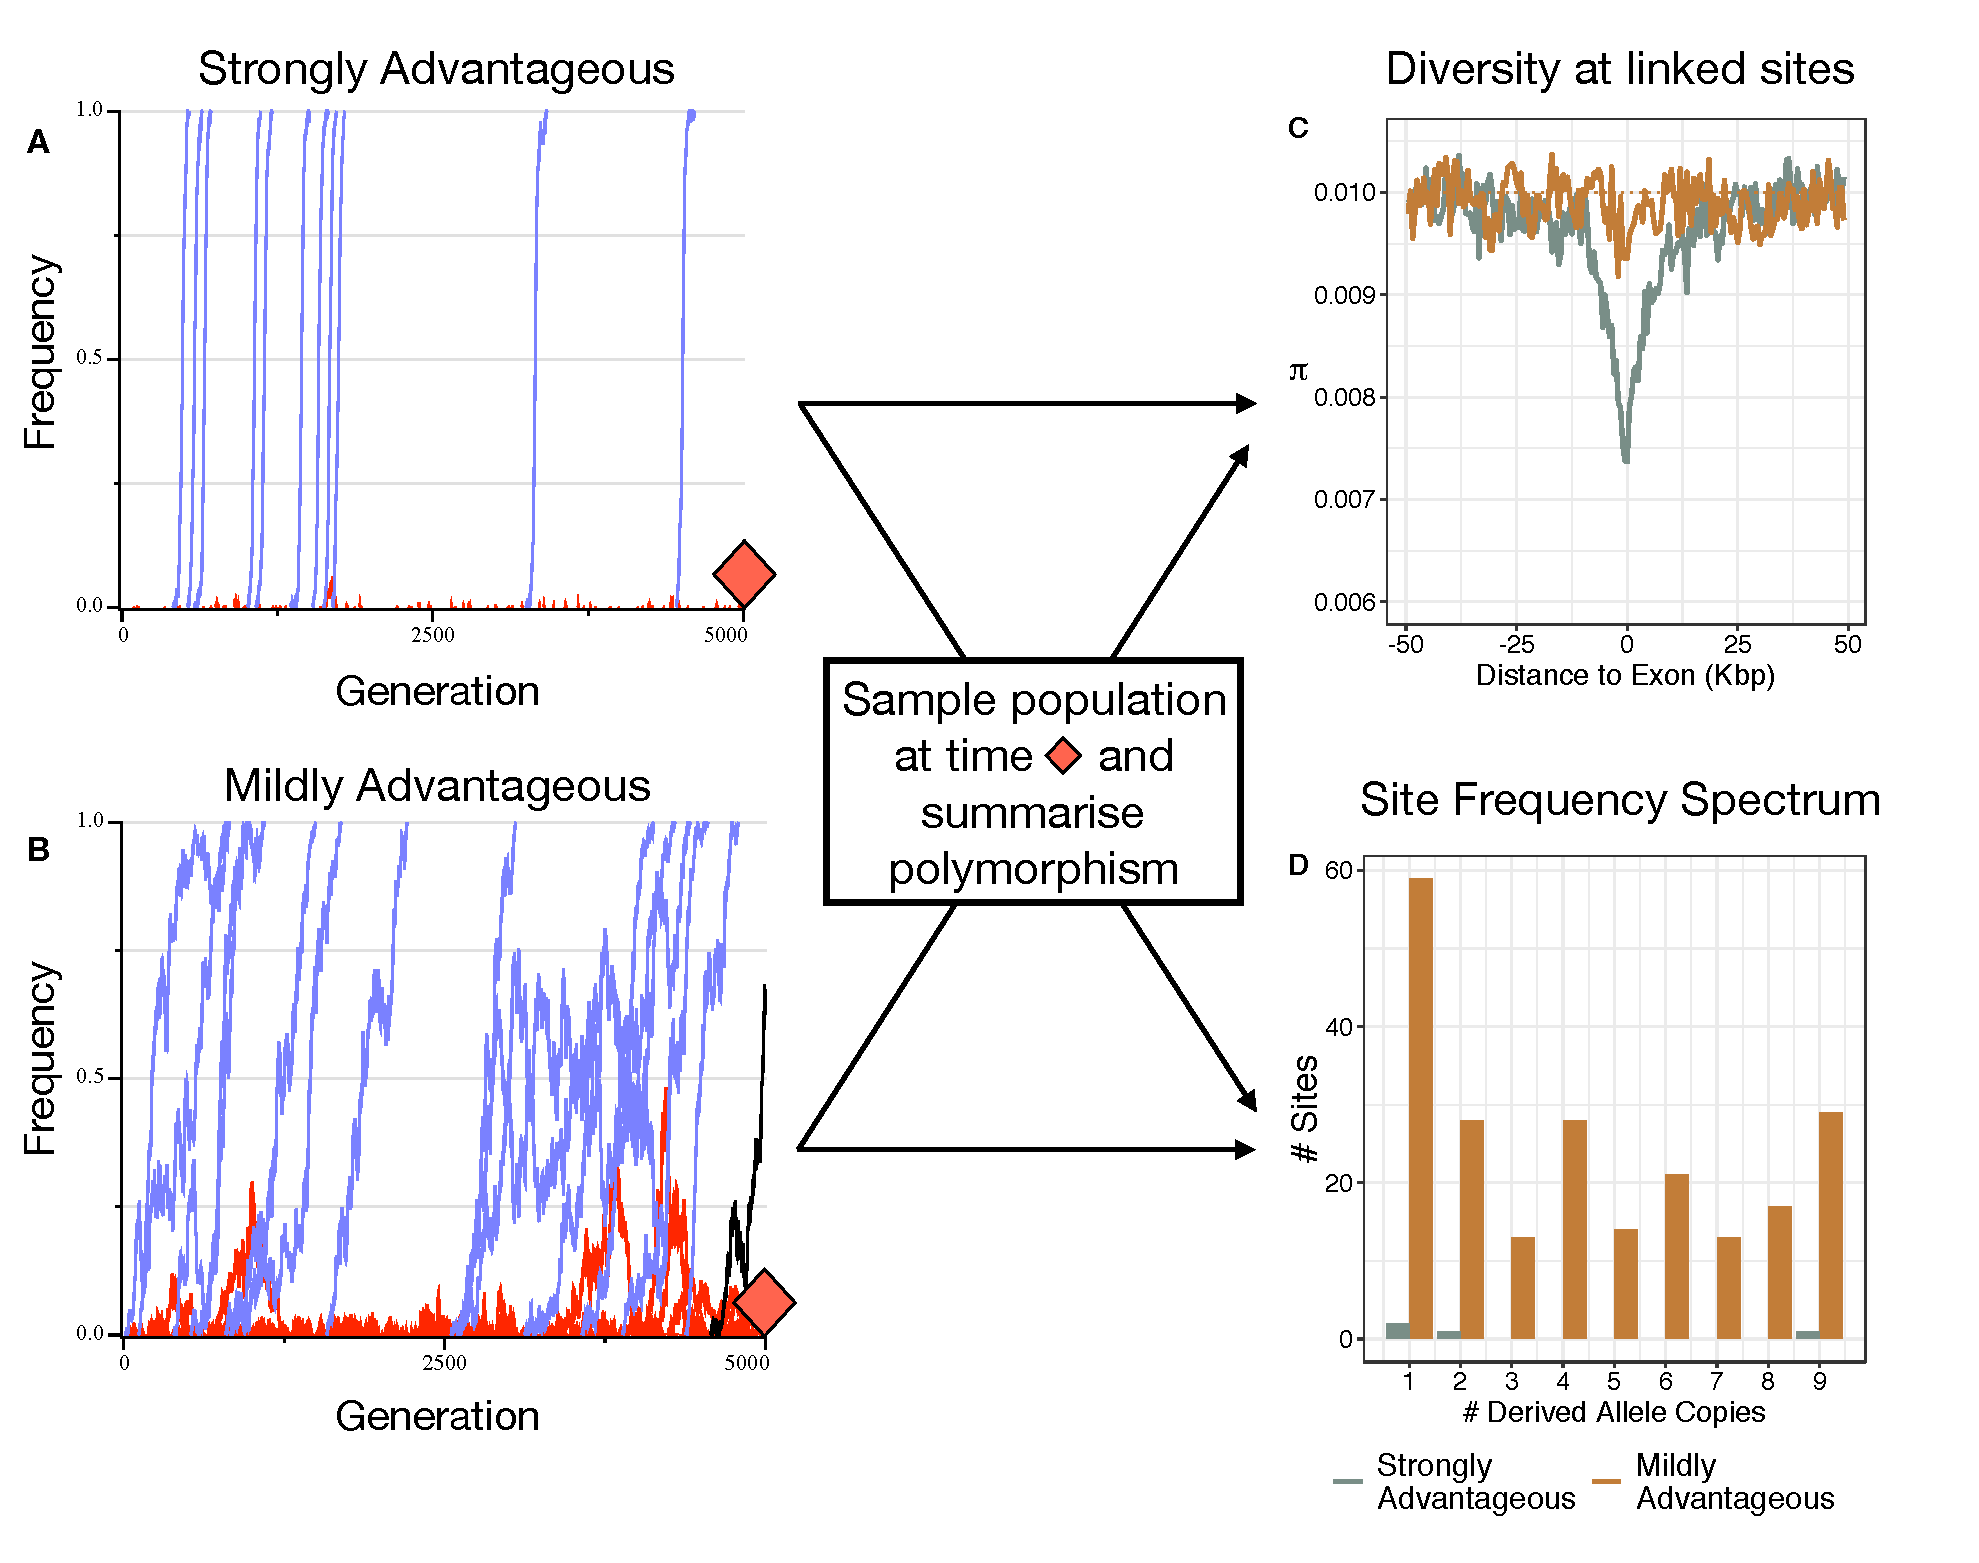
\includegraphics[width=\textwidth]{\dir/chapter4/figures/Trajectories.pdf}}
   
 \caption{A cartoon demonstrating the effect of strongly and mildly advantageous mutations on different aspects of population genomic data. A and B show frequency trajectories for advantageous mutations occurring in a simulated protein-coding exon. The case of infrequent, strongly selected advantageous mutations ($\gamma_a = 400$ and $p_a = 0.00025$) is shown in A. The case of frequent, mildly beneficial mutations ($\gamma_a = 10$ and $p_a = 0.01$) is shown in B. Note that the compound parameter $\gamma_a p_a$, which is directly proportional to the rate of selective sweeps, is the same for the two scenarios. In A and B blue lines represent mutations that went to fixation, red lines are mutations that were lost through drift and black lines are mutations that were polymorphic at the end of the simulation. Panel C shows the reduction in neutral diversity in regions surrounding a 1,000bp exonic region. D shows the site frequency spectra for advantageous mutations. Simulations were performed using the SLiMgui available at https://messerlab.org/slim/.}.
 
 \label{fig:Cartoon}
\end{figure}
\linespread{2}

	In Chapter 3, we sought to tease apart the contributions of BGS and SSWs to patterns of diversity in mice. By analysing unfolded site frequency spectra (uSFS), we estimated positive selection parameters, but found that these could not explain the troughs in nucleotide diversity around functional elements in the mouse genome. One explanation for our findings is that infrequent, strongly advantageous mutations, which may substantially influence diversity at linked sites, will make little contribution to standing variation and are thus undetectable by analysis of the uSFS \citep{RN290}. Figure \ref{fig:Cartoon} demonstrates how, for a given rate of sweeps, frequent mildly or infrequent strongly selected advantageous mutations may influence different aspects of population genomic data. The frequency trajectories in Figure \ref{fig:Cartoon} clearly show how weakly selected mutations take longer to fix and contribute more to standing variation than do strongly selected mutations. Furthermore, Figure \ref{fig:Cartoon} shows how strongly selected mutations in the population result in a marked reduction in diversity around the simulated exon, while contributing very little to standing variation (i.e. the uSFS). On the other hand, mildly advantageous mutations do not substantially affect linked diversity, but do contribute substantially to standing variation. Although only a cartoon, Figure \ref{fig:Cartoon} shows how, depending on the underlying parameters, different summaries of population genomic data are more or less informative for inferring positive selection. The methods we used in Chapter 3 relied on the assumption that selected mutations segregate in populations of interest, such that they affect the shape of the uSFS. Since the parameter estimates we obtained from the uSFS cannot explain the dips in diversity in mice, a more powerful approach for inferring the strength of positive selection may be to apply a model of selective sweeps to the observed data.
	
	In this study, we use a model of SSWs to estimate the strength and frequency of advantageous mutations in protein-coding exons and regulatory elements. Specifically, we find that the strength of selection acting on protein-coding exons is far greater than that acting on regulatory elements. Using simulations, we demonstrate that the inferred parameters of positive selection are likely out of the range detectable by analysis of the uSFS.  Finally, using a simple model of the fitness change brought about by adaptive evolution, we show that, despite adaptation occurring more frequently in regulatory regions, adaptation in protein-coding regions may contribute more to phenotypic evolution in mice.


%%%%%%%%%%%%%%%%%%%%%%%%%%%%%%%%%%%%%%%%%%%%%%%%%%%%
%
% #   #  ####  #####  #   #  ####    ####
% ## ##  #       #    #   #  #   #   #  
% # # #  ###     #    #####  #   #   ####
% #   #  #       #    #   #  #   #      #        
% #   #  #       #    #   #  #   #      #
% #   #  ####    #    #   #  ####    ####
%
%%%%%%%%%%%%%%%%%%%%%%%%%%%%%%%%%%%%%%%%%%%%%%%%%%%%
\section{Materials and Methods}

\subsection{Model of selective sweeps with background selection}

	\cite{RN290} gave expressions for the neutral diversity expected under the combined effects of BGS and SSWs. The model of sweeps they assumed considers the case of a haplotype carrying a neutral mutation at site $k$. A new semi-dominant advantageous mutation with selection coefficient $s_a$ occurs at site $i$ on the haplotype and spreads to fixation, affecting a change in the frequency of the neutral allele. Recombination between sites $i$ and $k$ uncouples the neutral and selected alleles at rate $r_{i,k}$. The change in neutral diversity at site $k$ ($\Delta \pi_k$), relative to its expectation in the absence of selection ($\pi_0$) is given by
	
\begin{equation}
\label{piChange}
\frac{\Delta \pi_{k}}{\pi_{0}} \approx -(2N_e s_a)^{\frac{-4r_{i,k}}{s_a}} .
\end{equation}
	
	\noindent
Where $N_e$ is the effective population size. This approximation assumes that selection on the advantageous allele satisfies $N_es_a > 1$ such that the sweep can be treated deterministically following its escape from drift. See \cite{RN235}, \cite{RN173}, or \cite{RN290} for a full derivation of Equation \ref{piChange}. 
		
	Equation \ref{piChange} can be thought of as the probability that a neutral allele is caught in the sweep, or as the probability of sweep-induced coalescence. For a particular class of functional elements (e.g. protein-coding exons), sweeps occur at a rate of $V_{a} = 2 \mu p_{a} \gamma_{a}$  per nucleotide per generation \citep{RN384}, where $\mu$ is the point mutation rate per nucleotide, $p_a$ is the proportion of new mutations that are advantageous and $\gamma_a$ is the scaled selection coefficient ($2N_es_a$) of those mutations. If $V_a$ is sufficiently low, such that one sweep does not interfere with another, the total probability of sweep-induced coalescence for a neutral site caused by selection at a linked functional element is
	
\begin{equation}
\label{singleClass}
P_{sc,k} \approx V_a \tau\gamma_a^{\frac{-4r_{i,k}}{s_a}}.
\end{equation}

\noindent
Where $\tau$ is the average number of sites in a particular class of functional elements. This model assumes that $N_e$ has remained constant for the timescale of the effects of sweeps and that there is full recovery of diversity between sweeps. When assuming that recombination proceeds solely by crossing over, $r_{i,k}$ is simply the product of the physical distance ($d_{i,k}$) and the local crossing-over rate ($r_c$). When incorporating gene conversion, we use Equation 1 from \cite{RN379}:
 
\begin{equation}
\label{geneConversion}
r_{i,k} = d_{i,k} r_c + 2 g_c d_g \Bigg( 1 - e ^{-\frac{d_{i,k}}{d_g}} \Bigg)
\end{equation} 
\noindent 
where $g_c$ is the rate of gene conversion and $d_g$ is the mean gene conversion tract length, assuming that the distribution of tract lengths is exponential. When applying Equation \ref{geneConversion} we use $g_c = \kappa r_c$ where $\kappa$ is the ratio of the non-crossovers to crossovers.
	

	The effects of BGS can be thought of as a reduction in the effective population size at a neutral locus by some fraction $B_k$. The probability of coalescence for a neutral allele affected by BGS is thus $\frac{1}{B_k 2N_e}$. If it is assumed that BGS and SSWs are independent exponential processes, the rate of coalescence induced by the two is simply the sum of $\frac{1}{2N_e B_k}$ and $P_{sc,k}$. We scale the sweep effect $P_{sc,k}$ by $B_k$ to reflect the reduction in the fixation probability for a new advantageous mutation given the reduced $N_e$ under BGS \citep{RN349}. Taking the reciprocal of the rate of coalescence at the neutral site given the combined effects of BGS and SSWs ($T_k$) and expressing it relative to the expected rate of coalescence under neutrality ($T_0$) gives

\begin{equation}
\label{jointApprox}
\frac{T_k}{T_0} \approx \frac{\pi_{k}}{\pi_{0}} \approx  \frac{1}{B_{k}^{-1}  + 2N_eB_{k}P_{sc,k}}.
\end{equation}
\noindent
	Where $\pi_k$ is genetic diversity observed at neutral site \textit{k} and $\pi_0$ is diversity expected in the absence of selection at linked sites. 
	
	Both theoretical and experimental results suggest that the distribution of fitness effects for advantageous mutations is exponential \citep{RN109}. We incorporate an exponential distribution of advantageous mutational effects in Equation 3 as follows:

		\begin{equation}
		\label{exponential}
P_{sc,k} \approx \int \limits_{0}^{\infty} f(\gamma_a) V_a \tau\gamma_a^{\frac{-4r_{i,k}}{s_a}} \mathop{d\gamma_a}.
		\end{equation}

	We estimated $\gamma_a$ and $p_a$ by fitting Equation \ref{jointApprox} to the relationship between nucleotide diversity and genetic distance to functional elements using non-linear least squares with the \emph{lmfit} (0.9.7) package for Python 2.7. When analysing the mouse data (\textit{see below}) we compared the fit of Equation \ref{jointApprox} incorporating either one or two discrete classes of advantageous mutations (Equation \ref{singleClass}) or the exponential distribution (Equation \ref{exponential}) using Akaike's Information Criterion (AIC). In the context of nonlinear least squares, the quantity being minimised is the sum of squares about the curve. Under a given model, if a normal distribution of residuals about the curve estimated by least squares is assumed, then the AIC can be calculated from the maximum likelihood estimated of the residual variance (pg60-64 of \citealt{RN393}). Standard errors in nonlinear least squares are derived from the covariance matrix of the best-fitting parameters.
		
	\subsection{Analysis of mouse data}

	We analysed patterns of genetic diversity in 10 wild-caught \textit{M. m. castaneus} individuals, first reported by \cite{RN122}. Briefly, \cite{RN122} sequenced individual genomes to high coverage ($\sim$ 30x) using Illumina paired-end reads, which were then mapped to the mm9 mouse reference genome using BWA \citep{RN251}. Variants were called using a Samtools pipeline \citep{RN252}. Note that we only analyse SNP data in this study, and insertion/deletion variants are not included. For further details of the sequencing and variant calling methods, see \cite{RN122}. Protein-coding exons annotated in version 67 of the Ensembl annotation database, and the locations of conserved non-coding elements (CNEs) identified by \cite{RN122} using an alignment of placental mammals, were used in this study. The mean length of a protein-coding exon is 151bp, of which we assume 75\% are subject to selection. The mean length of a conserved non-coding element is 51bp, of which 100\% of sites are assumed to be subject to selection.

	From the edges of exons (CNEs), polymorphism data and divergence from the rn4 rat reference genome were extracted for non-CpG-prone sites in windows of 1Kbp (100bp) extending to distances of 100Kbp (5Kbp). Non-CpG-prone sites were operationally defined as those that are either preceeded by a C or suceeded by a G in either the 3' to 5' or 5' to 3' directions in the reference genome. Analysis windows were then binned based on genetic distance to the focal element. Genetic distances were calculated using either the linkage disequilibrium (LD) based recombination map for \textit{M. m. castaneus} constructed by \cite{RN340} or the pedigree-based genetic map constructed using common lab strains of \textit{M. musculus} by \cite{RN232}. Because LD-based and pedigree-based recombination maps have different advantages and shortcomings (\textit{see Results}), we performed analyses based on both of these maps in parallel.

	Compared to crossingover rates, gene conversion parameters are very difficult to estimate \citep{RN247}. Empirical estimates of the ratio of crossovers to non-crossovers (a parameter we have termed $\kappa$) vary by orders of magnitude in mammals \citep{RN247}. \cite{RN263} measured non-crossover gene conversion rates in three recombination hotspots in mice and estimated a mean gene conversion tract length of 144bp and $\kappa = 0.105$, we refer to this estimate as the low gene conversion rate. \cite{RN263} pointed out that they likely underestimated the gene conversion rate. Since values of $\kappa$ as high as 12.0 have been reported in humans \citep{RN247}, we explored the effects of high gene conversion rates on the parameters of SSWs inferred from models of selection at linked sites, by also assuming $\kappa$ = 12.0, which we refer to as the high gene conversion rate. 

	In order to disentangle the sweep parameters we obtained by fitting Equation \ref{jointApprox}, we assume a point mutation rate of $5.4 \times 10^{-9}$, which is based on a mutation-accumulation experiment in \textit{M. musculus} \citep{RN228}. We also assume an $N_e$ for \textit{M. m. castaneus} of 426,200, based upon the level at which neutral diversity plateaus in the regions surrounding CNEs.

	\subsection{Estimates of \textit{B}} 
 
 	BGS contributes to the troughs in diversity around both protein-coding exons and CNEs (\citealt{RN122}; Chapter 3). We therefore required estimates of the effect of BGS on neutral diversity, \textit{B}, to use as a covariate when fitting Equation \ref{jointApprox} to diversity troughs. Analytical formulae for calculating \textit{B} over-predict the effects of BGS when purifying selection is weak ($\gamma_d < 1$) \citep{RN380,RN378}, and since weakly deleterious mutations comprise a large portion of the DFEs estimated for mice (\citealt{RN122}, Chapter 3), we opted to obtain \textit{B} from simulations.
 	
 	In Chapter 3, we used simulations to estimate the contribution of BGS to patterns of nucleotide diversity around both protein-coding exons and CNEs. We incorporated the actual distribution of the protein-coding genes (modelling both exons and untranslated regions) as well as CNEs into our simulations. The dDFEs we estimated for the 0-fold sites, untranslated regions and CNEs in Chapter 3 were incorporated into the simulations. Recombination rate variation was included in simulations assuming the \textit{castaneus} map. Simulations of $N = 1000$ diploid individuals were run for 10,000 generations. At the endpoint of simulations, we sampled 200 haploid chromosomes from the population and extracted $B = \frac{\pi}{\pi_0}$ as a function of genetic distance from both protein-coding exons and CNEs. We used these estimates of \textit{B} when fitting Equation \ref{jointApprox}. The simulations described here were identical to those we used in Chapter 3, except that we increased the number of simulation replicates from 2,000 to 6,000. 
 	
 	To obtain smoothed $B$ values we fitted Loess curves to the simulation data using R (v3.4.2), using a span parameter of 0.2 and using the number of sites contributing to each analysis bin as weights. Simulations were performed in SLiM (v1.8; \citealt{RN148}). 

	\subsection{Simulating the unfolded site frequency spectra}
	
	Figure \ref{fig:Cartoon} demonstrates that, for given rate of sweeps, different aspects of population genomic data may be informative for inferring positive selection if advantageous mutations occur frequently, but have mild fitness effects, or are infrequent, but are strongly beneficial. In Chapter 3 of this thesis, we estimated the frequency and strength of selection acting on advantageous mutations in \textit{M. m. castaneus} by analysing the uSFS, but found that the parameter estimates we obtained could not explain troughs in diversity observed around either protein-coding exons or CNEs. A possible explanation for our inability to explain the observed patterns is that the advantageous mutations involved are strongly selected and infrequent, and are thus difficult to estimate by analysis of the uSFS (see Introduction).
		
	We tested the hypothesis that infrequent, strongly advantageous mutations are difficult to detect by analysis of the uSFS using simulations. We generated simulated datasets using the forward-time simulation package SLiM (v1.8; \citealt{RN148}). We simulated the evolution of 1Mbp chromosomes containing 20 evenly spaced  `genes`. Each `gene` consisted of ten 100bp exons, separated by 1Kbp of neutrally evolving intronic sequence. We modelled nonsynonymous mutations as 75\% of mutations occurring in exons, and the remaining 25\% were strictly neutral (i.e. synonymous sites). We varied the $\gamma_a$ and $p_a$ parameters across simulations, but kept the product $\gamma_a p_a$ equal to 0.1. We based this value of $\gamma_a p_a \approx 0.1$ on a recent study of \textit{D. melanogaster} \citep{RN321}. All simulations incorporated the same gamma dDFE (shape parameter $\beta$ = 0.2 and mean $\hat{\gamma_d}$ = -1,000), but the advantageous mutation parameters varied, and are listed in Table \ref{tab:polyDFE} in the Results section. The population-scaled mutation and recombination rates (i.e. $\theta$ = \emph{$4N_{e}\mu$} and $\rho$ = \emph{$4N_{e}r$}, respectively) were set to 0.01. Populations of $N$ = 1,000 diploid individuals were simulated for an initial burn-in of 10$N$ generations to establish equilibrium conditions. After the burn-in, 20 haploid chromosomes were sampled every 2$N$ generations for a further 100$N$ generations. We performed 10 replicate simulations for each set of selection parameters. Across simulation replicates, time-points and loci we extracted simulated nonsynonymous and synonymous sites, giving uSFS data for 10,000 `genes'. We sampled the set of 10,000 `genes' with replacement 100 times, collating the nonsynonymous and synonymous site uSFSs for each replicate.
	
	We estimated our simulated DFEs by analysis of the uSFS using the methods of \cite{RN354}, as implemented in the polyDFE (v1.1) package. polyDFE fits an expression for the uSFS expected in the presence of both advantageous and deleterious mutations to data from putatively neutral and selected classes of sites, and estimates parameters by maximum likelihood. The neutral class is used to determine distortions to the uSFS caused by processes such as selection at linked sites and a history of population size change. In addition, polyDFE corrects for polymorphism misattributed to divergence, mutation rate variability and error in assigning sites as ancestral/derived. \cite{RN354} performed extensive simulations and showed that accurate estimates of the parameters for both deleterious and advantageous mutations can be obtained using their methods. However, there are a range of parameters that they did not test which may be biologically relevant, specifically when advantageous mutations are strongly selected, but infrequent.

	 We analysed the simulated uSFS data using polyDFE choosing Model C (a gamma dDFE and a discrete class of advantageous mutations) and either including or not including between-species divergence. We analysed the uSFS for simulated nonsynonymous sites using synonymous sites as the neutral reference class. For each of the advantageous mutation parameter sets tested, we analysed 100 bootstrap samples of the simulation data.
 
 	
%%%%%%%%%%%%%%%%%%%%%%%%%%%%%%%%%%%%%%%%%%%%%%%%%%%%
%
% ####   ####  #####  #   #  #     #######  #####
% #   #  #     #      #   #  #        #     #
% ## #   ###   #####  #   #  #        #     #####
% # #    #         #  #   #  #        #         #
% #  #   #         #  #   #  #        #         #
% #   #  ####  #####  #####  #####    #     #####
%
%%%%%%%%%%%%%%%%%%%%%%%%%%%%%%%%%%%%%%%%%%%%%%%%%%%%


\section{Results}

\subsection{Patterns of genetic diversity around protein-coding exons and conserved non-coding elements}


	In this study, we analysed the relationship between nucleotide diversity and genetic distance from functional elements in \textit{M. m. castaneus} assuming either a high resolution recombination map constructed using LD (Chapter 2; \citealt{RN340}) (the \textit{castaneus} map) or a pedigree-based map \citep{RN232} (the Cox map). The two methods for constructing recombination rate maps have advantageous and disadvantages. For example, the population-scaled recombination rate ($\rho$) can be inferred from a relatively small sample of unrelated individuals at very fine-scales using LD. However, selection at linked sites influences local LD and may therefore affect recombination rate estimates obtained in this way \citep{RN370}. Alternatively, direct estimates of the recombination rate ($r$) can be obtained from crossing experiments, but to achieve a high resolution recombination map a very large number of individuals need to be genotyped, and this has typically precluded the use of whole-genome re-sequencing, thereby limiting resolution. When analysing patterns of genetic diversity under a model of selection at linked sites, the way in which recombination rate estimates were obtained may, therefore, affect parameter estimates.

	Polymorphism data were extracted from genomic windows surrounding protein-coding exons and CNEs, genetic distances to focal elements were calculated assuming either an LD-based or a pedigree-based recombination map. The choice of recombination map used had a substantial effect on patterns of nucleotide diversity around both protein-coding exons and CNEs (Figure \ref{fig:Diversity2x2}). In the immediate flanks of both exons and CNEs, we found that diversity was lower when assuming the LD-based \textit{castaneus} map than when assuming the pedigree-based Cox map (Figure \ref{fig:Diversity2x2}). Note that we excluded analysis windows where $\rho<1$. Additionally, genetic diversity plateaued at higher levels (Figure \ref{fig:Diversity2x2}). These differences are consistent with the possibility that the Cox map, which was constructed with a far smaller number of markers than the \textit{castaneus} map, does not fully capture regions with both low and high recombination rates. A consequence of this would be, for example, that analysis windows tightly linked to functional elements appear less tightly linked. The choice of recombination map will, therefore, have an impact on the parameters of selection inferred from the patterns of diversity shown in Figure \ref{fig:Diversity2x2}. Throughout the rest of this chapter, we present the results of analyses based on the \textit{castaneus} map together with those based on the Cox map.

\linespread{1}
\begin{figure}[h!]
   \centering      
   \noindent\makebox[\textwidth]{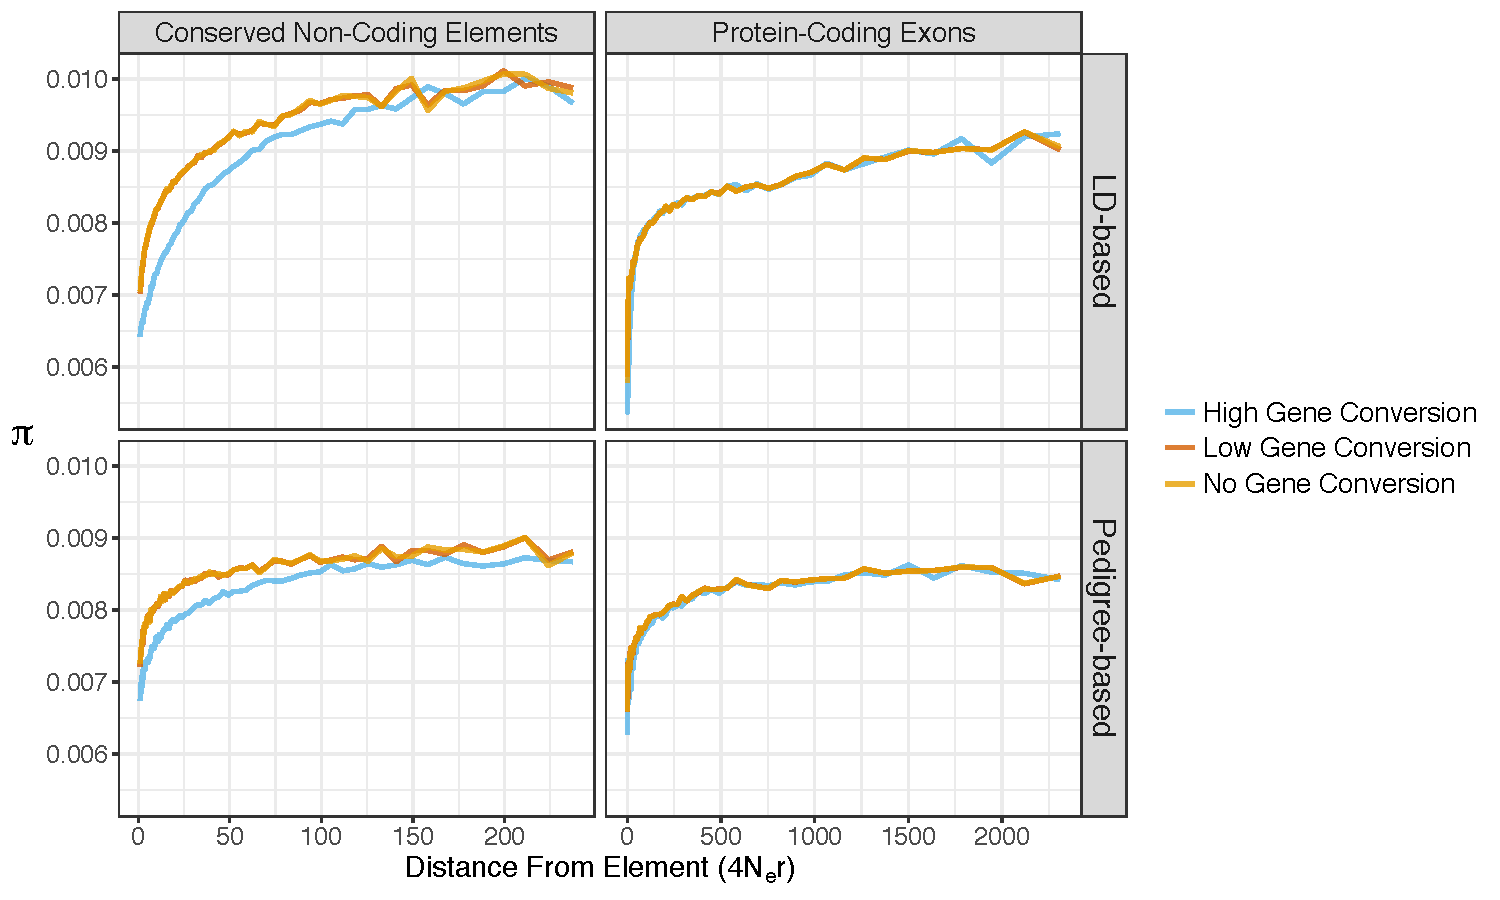
\includegraphics[width=\textwidth]{\dir/chapter4/figures/Pi_geneticDistance_4x4.pdf}}
 \caption{Nucleotide diversity in regions surrounding protein-coding exons and conserved non-coding elements in wild mice, assuming different rates of gene conversion. Population-scaled genetic distances ($4N_er$) were calculated using either an LD-based recombination map constructed for \textit{M. m. castaneus} or a pedigree based genetic map constructed for \textit{M. musculus}. Note that the lines for the cases of no gene conversion and low gene conversion are highly similar.}.
 
 \label{fig:Diversity2x2}
\end{figure}
\linespread{2}

	 Assuming the gene conversion parameters estimated by \cite{RN263} (i.e. a low gene conversion rate) had little effect on the patterns of genetic diversity around both classes of element (Figure \ref{fig:Diversity2x2}). Assuming a higher rate of gene conversion (i.e. 12 times the number of noncrossovers to crossovers) made more of a difference, particularly for CNEs (Figure \ref{fig:Diversity2x2}). The reason for this is that gene conversion will increase the recombination distance between two points proportionally more if analysis windows are physically short than if they are long (Equation \ref{geneConversion}) and the reductions in diversity around CNEs are about 10 times narrower than those around exons on a scale of physical distance \citep{RN122}. 
	 	 
\subsection{Diversity expected in the absence of selection, $\pi_0$}

	A key parameter in the model of SSWs and BGS investigated in this study is $\pi_0$, the nucleotide diversity expected in the absence of selection at linked sites. This parameter is very difficult to estimate and may even prove unobservable to be in real data given the ubiquity of selection effects at linked sites \citep{RN357}. One strategy for estimating $\pi_0$ is to divide the mean $\pi$ in regions distant from functional elements by the corresponding value of $B$, the reduction in neutral diversity caused by BGS. $B$ plateaus at approximately 0.95 in regions surrounding both protein-coding exons and CNEs (Figure {\ref{fig:BGSLoess}), but the level at which observed diversity plateaus is different for the two classes of elements (Figure \ref{fig:Diversity2x2}). It may be, then, that the diversity reducing effects of SSWs at elements linked to exons have been greater than for elements linked to CNEs. Because of this difference, and the similarity in BGS effects around the two classes of sites, simply dividing observed $\pi$ by $B$, would give an underestimate of $\pi_0$ as it would not incorporate the reduction in diversity caused by SSWs at linked elements. In addition, the levels at which diversity plateaus in the regions surrounding protein-coding exons and CNEs differ depending on which recombination map is assumed (Figure \ref{fig:Diversity2x2}).	When analysing patterns of diversity around protein-coding exons, we assumed $\pi_0$ values of 0.00955 and 0.00895 when analyses were based on the \textit{castaneus} and Cox maps, respectively. When analysing patterns of diversity around CNEs, we assumed $\pi_0$ values of 0.0102 and 0.00915 when analyses were based on the \textit{castaneus} and Cox maps, respectively.

\subsection{Parameters of selective sweeps obtained from patterns of nucleotide diversity}

	We fitted a model of SSWs and BGS to the reductions in diversity around exons and CNEs, and found that two classes of advantageous mutational effects typically gave a substantially better fit to the data than did a single class or an exponential distribution (as judged by AIC differences; Table \ref{tab:AICcomparison})). This result held regardless of the recombination map assumed and whether or not gene conversion was included. The only exception was that an exponential distribution gave the best fit when protein-coding exons were analysed using the \textit{castaneus} map with the high gene conversion rate, but in this case the AIC differences between the competing models were fairly small (Table \ref{tab:AICcomparison}).
	
\linespread{1}
\begin{table}[H]
   \centering
      \begin{threeparttable}[b]
\caption{Differences in fit for models of advantageous mutations when fitted to troughs in diversity around CNEs or protein-coding exons. Cells with no values indicate the best-fitting models.}


\begin{tabular}{ccccc}
\toprule
	& & & \multicolumn{2}{c}{$\Delta AIC$} \\
       Map & GC & Model\tnote{a} &  CNEs &  Exons \\
\midrule
 \multirow{9}{*}{\textit{castaneus}} &    \multirow{3}{*}{High} &     2 &       &        \\
  &      &     e &   -367 &    -284 \\
  &      &     1 &    -85.6 &    -284 \\ \cdashline{2-5}
  &     \multirow{3}{*}{Low}  &     2 &       &        \\
  &      &     e &   -280 &    -134\\ 
  &      &     1 &   -113 &    -161\\ \cdashline{2-5}
  &     \multirow{3}{*}{None}  &     2 &       &        \\
  &      &     e &   -262 &    -127 \\
  &      &     1 &    -87.3 &    -153 \\ 
\hdashline
\multirow{9}{*}{Cox}  &     \multirow{3}{*}{High} &     2 &       &      -3.91\\
  &      &     e &   -177&        \\
  &      &     1 &    -92&      -1.48\\ \cdashline{2-5}
  &     \multirow{3}{*}{Low} &     2 &       &        \\
  &  	 &     e &   -147 &     -16.2\\
  &      &     1 &    -43.5 &     -32.1\\ \cdashline{2-5}
  &     \multirow{3}{*}{None} &     2 &       &        \\
  &      &     e &   -150&     -19.6\\
  &      &     1 &    -44.0&     -38.9\\ 
\bottomrule
\end{tabular}
 
   \begin{tablenotes}
     \item[a] Denotes the model of advantageous mutations used. $e$ - exponential, $2$ - two classes of discrete effects and $1$ - a single class of discrete effects.
   \end{tablenotes}
  \label{tab:AICcomparison}

  \end{threeparttable}
  
\end{table}
\linespread{2}

	For both protein-coding exons and CNEs we inferred that there is a class of strongly advantageous mutations and a class of more mildly beneficial mutations (Table \ref{tab:EstimatesCastaneus}). When assuming the \textit{castaneus} map and the low gene conversion rate, we estimated the scaled effect of advantageous mutations ($\gamma_a$) was 8,470 and 432 for protein-coding exons and CNEs, respectively. The proportion of new mutations that possess these strongly advantageous selection coefficients were 2.2 x $10^{-5}$ and 1.12 x $10^{-3}$ for protein-coding exons and CNEs, respectively. We also inferred that there is a more mildly beneficial class of advantageous mutations affecting both protein-coding exons and CNEs, which had scaled effects of 22.3 and 14.5, respectively. The proportion of new mutations possessing the more mild selective effects were 0.0202 and 0.0298 for protein-coding exons and CNEs, respectively. With the \textit{castaneus} map, the inferred mildly beneficial mutation parameters were fairly similar to ones obtained by analysis of the uSFS in Chapter 3. Despite two classes of advantageous mutational effects giving the best fit to the CNE data when assuming the Cox map, the estimated standard errors for the mildly selected class are very large, so the evidence for mildly beneficial mutations is fairly weak in that case (Table \ref{tab:EstimatesCastaneus})

\linespread{1}


\begin{sidewaystable}[H]
\caption{Parameters of positive selection in \textit{M. m. castaneus} estimated by fitting a model of selective sweeps to troughs in diversity around functional elements. The frequency ($p_a$) and scaled selection coefficients ($\gamma_a$) for the two classes of advantageous effects are given. Parameters were obtained assuming background selection and the gene conversion parameters from \cite{RN263}. Standard errors are shown in square brackets below point estimates.}
\centering
	\label{tab:EstimatesCastaneus}
        \begin{tabular}{cccccc}

        \hline
  %            & \multicolumn{2}{c}{} & \multicolumn{2}{c}{}  \\
  Element  &  $\gamma_{a,1}$ & $p_{a,1}$ &$\gamma_{a,2}$ & $p_{a,2}$ &  \\ [0.5ex] \hline

\multirow{2}{*}{Protein-Coding Exons} &  8,470 & 2.22 x $10^{-5}$ & 22.3 & 0.0202 & \multirow{4}{*}{\textit{castaneus} map}\\
   &  [ 672 ] & [ 2.21 x $10^{-6}$ ]& [ 3.39 ] & [ 4.38x $10^{-3}$ ] & \\ 
\multirow{2}{*}{Conserved Non-Coding Elements}  & 432 & 1.12 x $10^{-3}$ & 14.5 & 0.0298 & \\
  &   [ 21.2 ] & [ 8.86 x $10^{-5}$ ]& [ 3.17 ] & [ 8.22 x $10^{-3}$ ] &\\ \hdashline
\multirow{2}{*}{Protein-Coding Exons} &  4,100 & 2.45 x $10^{-5}$ & 117 & 6.16 x $10^{-4}$  & \multirow{4}{*}{\textit{Cox} map}\\
   &  [ 640 ] & [ 5.56 x $10^{-6}$ ]& [ 49.9 ] & [ 2.78 x $10^{-4}$ ] & \\ 
   
\multirow{2}{*}{Conserved Non-Coding Elements}  & 357  &  4.77 x $10^{-4}$ & 5.95 & 0.0454 & \\
  &   [ 46.8 ] & [ 9.37 x $10^{-5}$ ]& [ 3.533 ] & [  0.0358 ] &\\ \hline
        \end{tabular}
   
\end{sidewaystable}


\linespread{2}	
	
	The choice of recombination map strongly affected the estimated selection parameters obtained by fitting patterns of genetic diversity. Use of the pedigree-based Cox map resulted in estimated selection coefficients that were typically smaller than the parameters obtained when assuming the LD-based \textit{castaneus} map (Table \ref{tab:EstimatesCastaneus}). This is presumably because we found the troughs in diversity around both classes of elements to be shallower when calculating genetic distances using the pedigree-based map than when using the LD-based map (Figure \ref{fig:Diversity2x2}).
	
	BGS contributes to the troughs in diversity around both protein-coding exons and CNEs, and causes an overall reduction in neutral diversity (Figure \ref{fig:castaneusFit}). Ignoring the contribution of BGS by setting $B$ to 1.0 when fitting Equation \ref{jointApprox} to the diversity troughs resulted in a much poorer model fit (Table \ref{tab:BGSeffect}). In the absence of BGS effects, the selection coefficents of advantageous mutations required to explain the observed data are far higher (Table \ref{tab:BGSeffect}), consistent with \cite{RN290}. 
	
\linespread{1}
\begin{figure}[h!]
   \centering      
   \noindent\makebox[\textwidth]{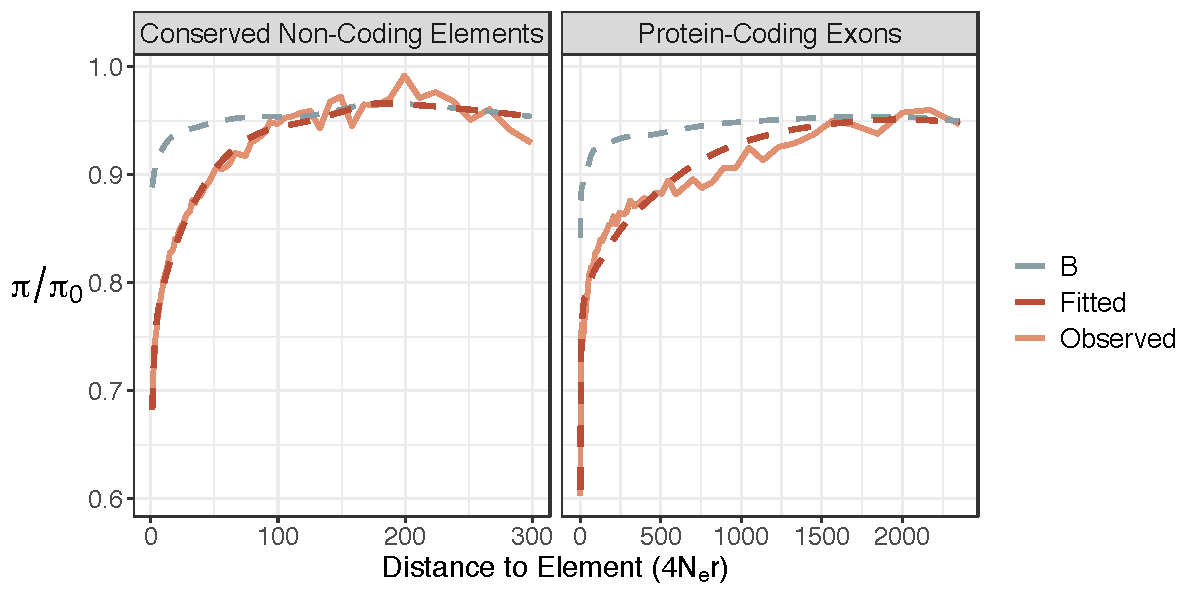
\includegraphics[width=\textwidth]{\dir/chapter4/figures/ModelFit.pdf}}
 \caption{The pattern of scaled nucleotide diversity around protein-coding exons and CNEs in \textit{M. m. castaneus} fitted using a model combining the effects of background selection and selective sweeps. Genetic distances were calculated assuming an LD-based recombination map constructed using population data from \textit{M. m. castaneus} and gene conversion parameters estimated by \cite{RN263}. The values of $B$ shown were from simulations.}  

 \label{fig:castaneusFit}
\end{figure}
\linespread{2}		
	The low rate of gene conversion that we assumed, which was estimated in \textit{M. m. domesticus}, did not substantially influence the outcome of our analyses (Table \ref{tab:GeneConversion}). This is presumably because gene conversion tracts, which are estimated to have a mean length of 144bp, will preserve little of the neutral diversity present in the population before the onset of a selective sweep. As sweeping alleles sojourn to fixation, a single crossover event affecting the sweeping haplotype may preserve much more neutral diversity than a small number of gene conversion tracts, so the effect of gene conversion on the troughs in diversity will be relatively small. We explored the effects of a high rate of gene conversion by setting the ratio of non-crossovers to crossovers to 12.0. In this case, the selection parameter estimates were substantially larger than the parameters obtained under either the low rate of gene conversion, or when assuming recombination proceeds solely by crossing-over, also consistent with \cite{RN290}. 
	
\subsection{Estimating selection parameters based on the uSFS of simulated data}

	Parameters of the DFE can be estimated directly from polymorphism data if selected mutations are segregating in the population of interest (\textit{reviewed in} \citealt{RN109}), and it has been repeatedly demonstrated that parameters of the DFE for deleterious mutations (dDFE) can be accurately estimated from the SFS \citep{RN201, RN164, RN178, RN354}. It has also been shown that the parameters of positive selection can be estimated from the uSFS \citep{RN210, RN354}, but it has also been argued that strongly selected advantageous mutations, which may contribute little to standing variation, will be undetectable by such methods (\citealt{RN290}; Chapter 3). In this study, we tested this verbal argument using simulations, showing that accurate estimation of positive selection parameters does indeed depend on the strength and relative frequencies of advantageous mutations. We used forward-in-time simulations that incorporated linkage, because selection at linked sites can distort the uSFS in ways that probably affect real data and thus cannot be ignored. For each set of advantageous mutation parameters, we simulated 10Mbp of gene-like sequences, giving a total of 7.5Mbp of nonsynonymous sites and 2.5Mbp of synonymous sites, which we used to construct the uSFS for 20 haploid individuals. This sample size and quantity of data are fairly typical of population genomic datasets (e.g. \citealt{RN236, RN238, RN368}). 

	Across simulations, the selection coefficients we simulated for advantageous mutations differed (ranging between $\gamma_a$ = 10 and $\gamma_a$ = 800), but the product $\gamma_a p_a$, which is directly proportional to the rate of sweeps, was always equal to 0.1. All simulations were subject to the same dDFE, so the extent of BGS should be fairly similar for all comparisons. We found that selection at linked sites reduced synonymous site diversity below the expected value of 0.01 in all simulations (Table \ref{tab:summaryStats}),  however as the strength of selection acting on advantageous mutations increased, diversity at linked sites decreased (reflected in the decreasing $\pi/\pi_0$ values shown in Table \ref{tab:summaryStats}). As expected, the relative fixation rate of nonsynonymous mutations (measured by $dN/dS$) did not vary systematically across simulations (Table \ref{tab:summaryStats}).

\linespread{1}

\begin{table}[h!]
   \centering
   \begin{threeparttable}[b]
\caption{Summary statistics for simulated populations. $\pi / \pi_0$ is diversity at simulated synonymous sites relative to neutral expectation. $dS$ and $dN$ are the proportions of substituted sites at simulated synonymous and nonsynonymous sites, respectively.}

\begin{tabular}{cccccc}
\toprule 
 \multicolumn{2}{c}{Simulated Value} &  \multirow{2}{*}{$\pi / \pi_0$} &  \multirow{2}{*}{$dS$} &  \multirow{2}{*}{$dN$} &  \multirow{2}{*}{$dN/dS$}     \\ \cline{1-2}
 $\gamma_a$ &       $p_a$ & & & &      \\
\midrule
       10 &  0.010000 &  0.940 &  0.00533 &  0.00159 &  0.299 \\
      20 &  0.005000 &  0.914 &  0.00526 &  0.00157 &  0.299 \\
      50 &  0.002000 &  0.880 &  0.00527 &  0.00159 &  0.302 \\
      100 &  0.001000 &  0.862 &  0.00525 &  0.00162 &  0.309 \\
     200 &  0.000500 &  0.844 &  0.00531 &  0.00159 &  0.300 \\
     400 &  0.000250 &  0.819 &  0.00523 &  0.00155 &  0.296 \\
     800 &  0.000125 &  0.795 &  0.00527 &  0.00156 &  0.295 \\
\bottomrule
\end{tabular}
\label{tab:summaryStats}

   \end{threeparttable}

   \end{table}
	
\linespread{2}

\linespread{1}

\begin{sidewaystable}[H]
\caption{Positive selection parameter estimates obtained by analysis of the uSFS for simulated populations. }
\medskip
\resizebox{\linewidth}{!}{%
\tabcolsep=2pt
\begin{tabular} { c | c c | c c | c c }

\toprule
 \multirow{2}{*}{Divergence \footnote{+/- indicates whether or not divergence was included when analysing the uSFS} } & \multicolumn{2}{c}{$\gamma_a$} & \multicolumn{2}{c}{$p_a$}  & \multirow{2}{*}{$\gamma_a p_a$} & Prop.\\
 	&    \textit{Simulated} & \textit{Estimated} & \textit{Simulated} & \textit{Estimated} &  &  Significant \footnote{The proportion of bootstrap replicates where a full DFE gave a significantly better fit than a model containing just deleterious mutations}\\
\midrule
         + &    \multirow{2}{*}{10} & 11.2 [5.60 - 20.0] &  \multirow{2}{*}{0.010000} & 0.00856 [0.00440 - 0.0199] &  0.0954 [0.0838 - 0.115] &  1.00 \\
         - &     & 3.97 [1.13 - 27.2] &   &         0.0201 [0.00472 - 0.0706] &  0.0828 [0.0616 - 0.155] &               1.00 \\ \hdashline
         + &   \multirow{2}{*}{20} &           16.6 [9.20 - 37.4] &  \multirow{2}{*}{0.005000} &  0.00568 [0.00241 - 0.0107] &  0.0949 [0.0822 - 0.108] & 1.00 \\
         - &    &        19.9 [2.90 - 37.4] &   & 0.00532 [0.00289 - 0.0207] &  0.106 [0.0454 - 0.193] &  0.97 \\ \hdashline
         + &   \multirow{2}{*}{50} &   37.4 [21.6 - 41.8] &  \multirow{2}{*}{0.002000} & 0.00257 [0.00202 - 0.00467] &  0.0951 [0.0809 - 0.106] & 1.00 \\
         - &    &   37.3[1.87 - 65.5] &  & 0.00266 [0.00125 - 0.0146] &  0.0717 [0.0112 - 0.145] &  0.86 \\ \hdashline
         + &   \multirow{2}{*}{100} &   37.43 [37.4 - 1530] &  \multirow{2}{*}{0.001000} &        0.00249 [0.0000738 - 0.00283] &   0.0938 [0.0795 - 0.107] &  1.00 \\
         - &    &  0.323 [0.0371 - 1.25] &   &  0.00259 [0.000525 - 0.0941] &  0.00102 [0.0000620 - 0.0137] & 0.00 \\ \hdashline
         + &  \multirow{2}{*}{200} &  37.4 [37.4 - 1,700] &  \multirow{2}{*}{0.000500} & 0.00251 [0.000220 - 0.00283] &     0.0947 [0.0738 - 0.106] & 1.00 \\
         - &   &            0.272 [0.00546 - 1.911] &   &                     0.0122 [0.000690 - 0.138] &  0.00310 [0.000104 - 0.0294] & 0.07 \\ \hdashline
         + &  \multirow{2}{*}{400} & 37.4 [32.7 - 37.4] &  \multirow{2}{*}{0.000250} & 0.00245 [0.00199 - 0.00283] &  0.0919 [0.0776 - 0.102] & 1.00 \\
         - &   & 12.3 [0.287 - 66.6] &   &  0.00212 [0.000783 - 0.0104] &  0.0338 [0.000250 - 0.0984] & 0.22 \\ \hdashline
         + &  \multirow{2}{*}{800} & 37.4 [32.9 - 37.4] &  \multirow{2}{*}{0.000125} & 0.00222 [0.00186 - 0.00264] &       0.0831 [0.0701 - 0.0936] & 1.00 \\
         - &   & 1.75 [0.111 - 43.0] &   &  0.00240 [0.000343 - 0.0293] &  0.0134 [0.0000515 - 0.0649] & 0.12 \\
\bottomrule
\end{tabular}}
  \label{tab:polyDFE}

\end{sidewaystable}

\linespread{2}


	 We analysed the uSFS obtained from our simulated populations and found that, when mutations were mildly advantageous ($\gamma_a$ $<$ 100) but relatively frequent ($p_a$ $>$ 0.0005), both $\gamma_a$ and $p_a$ parameters can be estimated with precision (Table \ref{tab:polyDFE}). However, we found that when advantageous mutations were strongly selected, but infrequent ($\gamma_a$ $\geq$ 100 and $p_a$ $\leq$ 0.0005), the parameters were very poorly estimated. Across all simulated datasets, when we analysed the uSFS, including sites fixed for the derived allele in the analysis, the product $\gamma_a p_a$ was accurately estimated (Table \ref{tab:polyDFE}) and likelihood ratio tests never failed to detect the presence of advantageous mutations in the uSFS. When we excluded sites fixed for the derived allele from the analysis, however, the product  $\gamma_a p_a$  was poorly estimated when $\gamma_a \geq 100$ and likelihood ratio tests typically failed to detect positive selection (Table \ref{tab:polyDFE}). 	 

	We found that the uSFS analysis methods of \cite{RN354} as implemented in polyDFE gave estimates of the dDFE which were highly accurate (Table \ref{tab:dDFE}), even when positive selection was very strong. Analysing simulated uSFSs with polyDFE yielded estimates of the dDFE that were extremely precise, although whether or not divergence was included and whether or not a full DFE was inferred affected parameter estimates. This is particularly evident for the case when $\gamma_a$ = 10 and $p_a$ = 0.01 (Table \ref{tab:dDFE}), where advantageous mutations contribute substantially to standing variation (Figure \ref{fig:SFSexample}). In this case, by limiting the inference to just the dDFE, advantageous mutations that contribute to the shape of the uSFS are assumed to be deleterious, resulting in spurious dDFE inferences. In the simulations where $\gamma_a$ = 800 and $p_a$ = 0.000125, advantageous mutations make little contribution to standing variation (Figure \ref{fig:SFSexample}, and the effect of not modelling a full DFE is less pronounced (Table \ref{tab:dDFE}).
	
%	 Across all simulations, we found that polyDFE gave estimates of the dDFE which were highly accurate (Table \ref{tab:dDFE}). polyDFE performed most poorly when divergence was included in the analysis, but only a dDFE was inferred. These results replicate the findings of \cite{RN354} and further emphasize the importance of specifying a full DFE model when making inferences of selection from the uSFS. 

%%%%%%%%%%%%%%%%%%%%%%%%%%%%%%%%%%%%%%%%%%%%%%%%%%%%
%
% ####  #  #####  #####  #   #    #####  #####
% #   # #  #      #      #   #    #      #
% #   # #  #####  #      #   #    #####  #####
% #   # #      #  #      #   #        #      #
% #   # #      #  #      #   #        #      #
% ####  #  #####  #####  #####    #####  #####
%
%%%%%%%%%%%%%%%%%%%%%%%%%%%%%%%%%%%%%%%%%%%%%%%%%%%%

\section{Discussion}

	There is now evidence that both BGS and SSWs operate in the mouse genome. By fitting a model of SSWs to the troughs in diversity around protein-coding exons and CNEs, assuming that part of the reduction is driven by BGS, we estimated parameters of positively selected mutations occurring in the two classes of element that can explain observed patterns of pairwise diversity at putatively neutral sites. We found that protein-coding regions experience more strongly selected mutations than do regulatory sequences. For both classes of sites, we found statistical support for two classes of advantageous mutational effects, one strong ($\gamma_a > 200$) and one comparatively weak ($\gamma_a < 150$). Using simulations, we demonstrated that it is difficult to accurately infer selection parameters using analyses which rely on the presence of advantageous mutations contributing to the uSFS. In such cases, patterns of diversity at linked sites, such as reductions in putatively neutral diversity near near functional elements, are perhaps a more useful summary of population genomic data from which to estimate parameters of selection.
	
	Our selection parameter estimates for \textit{M. m. castaneus} are fairly similar to estimates obtained for European \textit{M. m. domesticus} \citep{RN355}. \cite{RN355} analysed patterns of variation at microsatellite loci across the \textit{M. m. domesticus} genome using a model of SSWs and estimated that sweeps casued by mutations with a selection coefficient of $s \approx 0.008$ occur at least every hundredth generation, though they did not account for BGS. If we assume $N_e$ = 423,200 for \textit{M. m. castaneus}, we estimate that SSWs in protein-coding exons and CNEs are driven by strongly beneficial mutations with selection coefficients of approximately 0.010 and 0.0005, respectively (using the parameters of the strongly beneficial mutations obtained assuming the LD-based map). Our parameter estimates roughly correspond to  0.01 and 0.30 strong sweeps per generation for protein-coding exons and CNEs, respectively, so our estimates are broadly consistent with the lower bound from \cite{RN355}.
	
\subsection{The relative contribution of adaptive substitutions in protein-coding and regulatory regions to fitness change in mice}

	An enduring goal of evolutionary biology has been to understand the extent to which protein-coding and regulatory regions of the genome contribute to phenotypic evolution \citep{RN347, RN346}. \cite{RN347} posited that, since identity between human and chimpanzee proteins is around 99\%, changes in gene regulation may explain the plethora of phenotypic differences between the two species. If we assume that there is a simple relationship between fitness and phenotype, then using a simple model of the fitness change brought about by the substitution of advantageous mutations, we can use the parameter estimates we obtained in this study to try and understand the contributions of protein-coding and regulatory regions of the genome to phenotypic evolution.

	Consider the following model of the fitness change ($\Delta W$) brought about by the fixation of advantageous mutations. For a particular class of sites, of which there are $n_a$ nucleotides in the genome, new mutations occur at rate $\mu$ per nucleotide site, per generation. We assume that a proportion of those new mutations, $p_a$, are strongly advantageous with a selection coefficient of $s_a$. The advantageous mutations fix with probability $u(s_a)$ and once fixed contribute $s_a$ to the change in fitness. If selection is strong relative to genetic drift, then $u(s_a)$ is approximately $s_a$, giving the following expression:

		\begin{equation}
		\label{eq:fitness}
		\Delta W \propto \mu p_a n_a s_a^2,
		\end{equation}

	We parametrized Equation \ref{eq:fitness} using the selection parameters estimated in this study, summing the fitness contribution for the two classes of fitness effect. We assume that the average point mutation rate is the same for CNEs and protein-coding exons, and we can thus ignore $\mu$ in Equation \ref{eq:fitness}. 
 
	Based on our parameter estimates, we find that adaptation is far more frequent in regulatory regions than in protein-coding regions, but that protein-coding regions contribute more to fitness change. Firstly, there are about two to three times as many CNE bases as there are non-synonymous ones in the mouse genome \citep{RN122}, and secondly the frequency at which new advantageous mutations arise at CNEs is greater than for protein-coding exons (Table \ref{tab:EstimatesCastaneus}). Because of these two factors, the rate of advantageous mutations occurring in regulatory regions is likely to far exceed that of protein-coding regions. However, the average strength of selection acting on a new advantageous mutation in a protein-coding exon far exceeds that of a mutation in a CNE (Table \ref{tab:EstimatesCastaneus}) and since the change in adaptive fitness is dependant on the square of the selection coefficient, the change in population mean fitness brought about by the fixation of advantageous mutations is higher for protein-coding exons than for CNEs (Table \ref{tab:fitness}). The difference we found was small (around 3 times higher for protein-coding regions than for regulatory regions), but was robust to the choice of recombination map (Table \ref{tab:fitness}). 

\linespread{1}
\begin{sidewaystable}[H]
\caption{Estimates of the change in fitness brought about by the fixation of advantageous mutations ($\Delta$). Estimates were obtained using Equation \ref{eq:fitness} assuming the selection parameters shown in Table \ref{tab:EstimatesCastaneus}. }

\begin{tabular}{ccccccccccccc}
\toprule
       Map & Element &        $s^{2}_{a,1}$ &      $s^{2}_{a,2}$ &     Sites (Mbp) & $\Delta W_{a,1}$ &    $\Delta W_{a,2}$ &   $\Delta W_{a}$ & Ratio \\
\midrule
 \multirow{2}{*}{\textit{castaneus}} &    Exon  &  9.87 x $10^{-5}$  & 6.87 x $10^{-10}$  & 24.0 &  2.84 x $10^{-10}$  &  1.79 x $10^{-12}$  &  2.86 x $10^{-10}$  &  3.29 \\
  &     CNE  &  2.56 x $10^{-7}$ &  2.90 x $10^{-10}$  & 54.2 & 8.44 x $10^{-11}$  &  2.53 x $10^{-12}$  &  8.69 x $10^{-11}$  &         - \\ \hdashline
       \multirow{2}{*}{Cox} &     Exon  &  2.31 x $10^{-5}$ &  1.89 x $10^{-8}$  &  24.0 &  7.34 x $10^{-11}$  &  1.51 x $10^{-12}$  &  7.50 x $10^{-11}$ &  2.98 \\
        &     CNE  &  1.76 x $10^{-7}$ &  4.88 x $10^{-11}$  &  54.2 &  2.45 x $10^{-11}$  &  6.49 x $10^{-13}$  &  2.51 x $10^{-11}$ &         - \\
\bottomrule
\end{tabular}
 \label{tab:fitness}

\end{sidewaystable}

\linespread{2}

	There are a number of factors that should temper these conclusions, however. 	Firstly, we assumed fixed values for the selection coefficient that appears in Equation \ref{eq:fitness}. If there were a continuous distribution of $s$ values around the point estimates we obtained in this study, integrating over this distribution could yield a different result. Secondly, we have assumed that all elements of a particular class share a common set of selection parameters. This is slightly, problematic since there are a number of sub-categorisations that could be applied to the set of CNEs we analysed (e.g. promoters and enhancers may be subject to different selective pressures). Indeed, different categories of protein-coding genes may also be subject to different selection pressures. For instance, virus interacting proteins in humans and highly expressed genes in \textit{Capsella grandiflora} have been estimated to have higher rates of adaptive substitutions than the genome wide average \citep{RN236, RN777}.

	Whether or not the conclusions we have drawn in this study can be generalised to other organisms remains to be seen, but the brown rat, \textit{Rattus norvegicus}, provides a compelling first case for comparison. In \textit{R. norvegicus} there are troughs in nucleotide diversity around protein-coding exons and CNEs that are very similar to those observed in \textit{M. m. castaneus} \citep{RN327}. Since broad-scale recombination rates are similar in mice and rats \citep{RN184}, qualitatively similar conclusions regarding the contribution of protein-coding versus regulatory change to adaptive evolution may be reached when analysing patterns of genetic diversity in rats. 

\subsection{Estimating parameters of positive selection from the uSFS versus estimates from patterns of diversity}

	In this study, we fitted a model of selective sweeps to troughs in putatively neutral diversity surrounding protein-coding exons and CNEs in \textit{M. m. castaneus}, and found that strongly advantageous mutations explain the observed patterns. In Chapter 3, we analysed the uSFSs for the same classes of sites, but found only evidence for mildly advantageous mutations. The different approaches we took in this study and in Chapter 3 make use of different aspects of population genomic data, which are both informative about positive selection, but in differnet ways (Figure \ref{fig:Cartoon}). Two recent studies in chimpanzees provide a clear example of how different features of population genomic data can lead one to different conclusions regarding positive selection. Firstly, evidence, from between-species divergence, suggests that about 30\% of nonsynonymous substitutions in chimps were driven by positive selection \citep{RN215}. Because the rate of adaptive substitution is determined by the product of the strength of selection and frequency of advantageous mutations \citep{RN384}, the 30\% of nonsynonymous substitutions in chimps attributable to adaptation could be due to a relatively high rate of weakly advantageous mutations, or a low rate of strongly advantageous mutations. Recently, \cite{RN365} analysed population genomic data from chimps (as well as several other great ape species) and concluded that SSWs driven by strongly selected mutations were the cause of dips in diversity observed around protein-coding genes on the autosomes. \cite{RN354} analysed the uSFS for nonsynonymous and synonymous sites in chimps using polyDFE, but found little evidence for positive selection on the autosomes. The cartoon shown in Figure \ref{fig:Cartoon}, as well as our simulation results, demonstrate how strongly advantageous mutations affect different aspects of population genomic data, potentially reconciling the seemingly contradictory results of \cite{RN365} and \cite{RN354}. 

	In collating the patterns of genetic diversity around either CNEs or protein-coding exons across the entire genome, it is likely that we have lost some valuable information. In particular, we set $\pi_0$, nucleotide diversity expected in the absence of selection, when fitting a model combining the effects of SSWs and BGS (Equation \ref{jointApprox}), using values that gave a reasonable fit to the data, but did not explicitly model the reduction in genetic diversity caused by SSWs at linked elements.	An alternative approach would be to fit Equation \ref{jointApprox} to genome-wide variation in nucleotide diversity, conditioning on the locations of functional elements and the genetic map. \cite{RN274} performed such an analysis on polymorphism data from \textit{D. melanogaster} using a model that condiditoned the effects of SSWs on the locations of recent substitutions and the effects of BGS on the locations of functional elements. However, applying their methods to mice, where there is little difference between the patterns of mean diversity around putatively selected/neutral nucleotide substitutions \cite{RN122}, would probably result in spurious parameter estimates. 
		
	Increases in statistical power could possibly be made by analysing larger amounts of data when attempting to detect positive selection using the uSFS. In Chapter 3, for example, we excluded CpG-prone sites from our analyses as a conservative way to remove hyper-mutable CpG sites from the analysis, because the methods we used assume a single mutation rate. However, removing CpG-prone sites removed approximately 50\% of the available data. Increasing the number of sites or the number of sampled individuals may give more precise estimates of the uSFS and more power to infer selection coefficients, but based on the parameter estimates obtained in this study, very few strongly advantageous mutations would segregate in the mouse population at any given time, and uSFS-based analyses only work if selected mutations are segregating in the population. 

	The rate of fixation of advantageous mutations provides information on the product of the scaled strength of selection and frequency of advantageous mutations $\gamma_a p_a$ (Kimura and Ohta 1971). When there is little information present in the polymorphism data, this compound parameter cannot be used to separately estimate $\gamma_a$ and $p_a$. In our simulations, increasing $\gamma_a$, but decreasing $p_a$ such that the compound parameter stayed constant, we found that the ability to infer positive selection from uSFS on the basis of polymorphism alone decreased (Table \ref{tab:polyDFE}). In our analyses of the uSFS for wild mice in Chapter 3, we found statistically significant evidence for positive selection on the basis of polymorphism alone. In this study, we analysed patterns of genetic diversity at linked sites and estimated that there is a class of mildly advantageous mutation that occur in protein-coding exons. If the true DFE for advantageous mutations in mice contained a substantial fraction of mildly beneficial mutations, as our analyses in this study suggest (Table \ref{tab:EstimatesCastaneus}), then they should be reflected in the parameter estimates that we obtained by analysis of the uSFS in Chapter 3.

	To our knowledge, there are currently no methods that estimate the DFE using an analytical expression for the expected SFS under either BGS or SSWs. Rather, nuisance parameters or demographic models are used to correct for the contribution that selection at linked sites makes to the shape of the SFS, while assuming that selected mutations also shape the SFS. However, we have shown that advantageous mutations occurring in \textit{M. m. castaneus} may be far stronger and more infrequent than those that can reliably be detected by analysis of the uSFS. A way forward may be in using approximate Bayesian computation or machine-learning approaches to make use of all of the available data, while not having to have an expression for the uSFS expected under the combined effects of BGS, SSWs, population size change and direct selection.
		

\subsection{Choosing gene conversion parameters}

	There is little knowledge of how rates of gene conversion vary across the mouse genome. We have assumed a constant rate of gene conversion in this study, but whether or not this is biologically realistic is unknown. There is evidence that the spacing of gene conversion events are not restricted by interference in the same way as crossovers are \cite{RN263}, but beyond that, there is relatively little known about the variation in gene conversions rates across the mouse genome. We demonstrated that a high rate of gene conversion has the potential to substantially influence parameter estimates, but the rate based on the analyses of \cite{RN263} had little effect compared with no gene conversion (Table \ref{tab:GeneConversion}). In addition, the LD-based \textit{castaneus} map was constructed using a model of crossovers that does not explicitly model gene conversion (Chapter 2). However, gene conversion will affect LD and may be reflected in the estimates of $\rho$/bp obtained using LDhelmet. In particular, gene conversion may generate bias in LD-based recombination maps in regions of the genome with high marker density, because higher marker densities are required to detect gene conversion events (reviewed in \citealt{RN394}). It is conceivable that patterns of LD could be used to estimate rates of gene conversion across whole chromosomes, and applying such methods may provide further insight into the variation in recombination across mammalian genomes. Understanding how gene conversion rates vary across the genome would allow us to make more precise estimates of the parameters of selection.

\subsection{Hard versus soft selective sweeps}


	For both protein-coding exons and CNEs we found that a model that included two classes of advantageous mutational effects gave the best fit to the data. For a single class of advantageous mutational effects, the predicted reduction in diversity caused by selective sweeps is a simple logistic function (Equation \ref{jointApprox}). We found that the observed troughs in diversity around protein-coding exons and CNEs more closely resembled the curves expected under two different classes of advantageous mutational effects. However, the model of SSWs that we assumed in this study involves so-called `hard' (or `classic') sweeps, whereas studies in both humans and \textit{Drosophila} suggest that 'soft' sweeps are common \citep{RN208, RN303, RN338}. A 'soft' selective sweep occurs when an advantageous allele reaches fixation but drags multiple haplotypes to high frequencies, which can occur if selection acts on standing genetic variation or if multiple copies of the selected mutation arise independently \citep{RN336}. Additionally, adaptation acting on quantitative traits subject to stabilising selection may generate partial sweeps, because abrupt changes in allele frequency at many loci can rapidly alter mean phenotypes, without necessarily causing fixations \citep{RN147}. Such partial sweeps may be common in humans \citep{RN301}. The profiles of the reductions in diversity around soft and partial sweeps differ from those expected under hard sweeps, so if either of the alternative types of sweep were common, the assumption of a hard sweep model may result in spurious parameter estimates \citep{RN274}. It seems likely that adaptation does not fit any one category, rather different functional elements will be subject to a mixture of different types of sweep. In the case of a soft sweep from standing variation, for example, the effect on neutral diversity is related to the frequency with which the focal allele was segregating before the onset of selection. Since nonsynonymous variants are maintained at lower frequencies than variants within CNEs \citep{RN122}, the effects of soft sweeps may differ between the two classes of sites.

	
\section{Conclusions}

	In this study we have shown that that strong positive selection explains the diversity dips around protein-coding exons and CNEs. Using simulations, we showed that the parameters of these mutations are out of the range detectable by the uSFS, thus reconciling the present results with those obtained in Chapter 3. Furthermore, the parameters we estimated suggested that mutations in protein-coding regions may contribute slightly more to phenotypic change than do regulatory mutations.







	% Boot up the Chapter 5: Overall discussion
	\chapter{General Discussion}
\chaptermark{Discussion}

\section{Overview}

	The main aim of this thesis has been to increase our understanding of the factors that have shaped nucleotide diversity across the mammalian genome. To that end, I have focussed on understanding how processes of selection at linked sites contribute to variation in genetic diversity across the genome. Each of the projects described in the preceding three chapters have touched upon a different aspect of this. Here, I briefly summarise the main points, as regards selection at linked sites, that can be gleaned from the three projects I presented.

	In Chapter 2, I used a coalescent-based method to infer a recombination rate map from patterns of LD for \textit{M. m. castaneus}. I used this map to analyse the relationship between synonymous site diversity for protein-coding genes and local recombination rate. I found that putatively neutral diversity and recombination rate were positively correlated. Since both background selection and selective sweeps are expected to cause reductions in diversity, which are positively correlated to the rate of recombination, the relationship I found is indicative of the widespread effects of selection at linked sites. However, the positive correlation does not, on its own, carry information on the contributions of background selection and selective sweeps. The recombination map that I generated was important for the analyses performed in Chapters 3 and 4.
	
	In Chapter 3, I estimated the DFE for both harmful and advantageous mutations by analysing the unfolded site frequency spectrum (uSFS). Given the parameters obtained, I found that a combination of BGS and SSWs, could not fully explain the dips in diversity observed around functional elements in \textit{M. m. castaneus}. Using simulations, I found circumstantial evidence that selective sweeps, driven by strongly advantageous mutations, are a major contributor to the dips in putatively neutral diversity around functional elements in mice.

	In Chapter 4, I used a model that combined the effects of background selection and selective sweeps to estimate parameters of positively selected mutations that could generate the troughs in diversity observed around protein-coding exons and conserved non-coding elements (CNEs). My analyses suggested that strongly selected advantageous mutations in protein-coding exons are less frequent, but have substantially larger selection coefficients than those that occur in CNEs. Using the parameters, I found that the contribution to fitness change brought about by the substitution of advantageous mutations in protein-coding regions may somewhat outweigh that of advantageous mutations in regulatory elements.

	The main finding from the work I have carried out is that strongly advantageous mutations are chiefly responsible for the large troughs in diversity around both protein-coding exons and CNEs observed by \cite{RN122}. In Chapter 3, I showed that BGS makes a contribution to the observed troughs, but in Chapter 4 I showed that strong SSWs are required to fully explain them. I also presented evidence that, for at least two classes of functional sites in mice, there is a multimodal distribution of advantageous mutational effects. 
	 
\section{Limitations}

	There are a number of useful insights to be gleaned from the three projects described in this thesis, but the work I have done does not close the book on our understanding of selection in the house mouse genome. There are a number of assumptions that permeate this thesis, and here I give a brief description of these and the limitations they impose on the work carried out.
 
\subsection{Neutrally evolving sequences}

	 Probably the most obvious assumption I made is that that neutrality can be ascribed to certain classes of sites and regions of the genome. I made this assumption when analysing recombination rates in Chapter 2, the method I used (LDhelmet) invokes neutrality to model recombination rate variation across a chromosomal region \citep{RN213}. I also made this assumption in Chapter 3, where I assumed that the uSFSs for 4-fold and CNE-flanking sites represent neutrally evolving sequences. Although the sites may not themselves be the targets of selection, they may be influenced by selection at linked sites. There is ample evidence for selection acting on several classes of functional elements in the house mouse genome \citep{RN342, RN170} and for some classes of sites, this affects genetic diversity in surrounding genomic regions (\citealt{RN122}; Chapter 3). This will have influenced my efforts to estimate recombination rates and to estimate DFEs in Chapters 2 and 3, respectively.

\subsubsection{Recombination rate issues}

	The method used to infer recombination rate variation in Chapter 2, LDhelmet \citep{RN213}, is built upon coalescent theory, which makes the assumption that SNPs in a focal region are evolving neutrally. For a pair of SNPs, the likelihood of an observed genealogy under a particular recombination rate (in terms of $4N_er$) is calculated. By estimating the recombination rate between pair-wise combinations of SNPs, one can then build up a recombination map for a particular genomic region. Both population size change and selection at linked sites can influence linkage disequilibrium \citep{RN319}, distort genealogies away from neutral expectation \citep{RN192} and reduce the total number of segregating variants in a region \citep{RN287}. Both processes could, therefore, potentially bias and affect the resolution of recombination rate maps obtained using methods such as LDhelmet.
		
	Firstly, methods such as LDhelmet rely on the presence of SNPs, so a low number of variants in a region limits the resolution to which recombination rates can be inferred. The effects of population size change have recently been incorporated into the methodology \citep{RN381}, but this relies on accurate estimates of the demographic history of the population, which is not necessarily straightforward (\textit{see below}).
	
	Low recombination rates estimated from LD may be a caused by the effects of selection at linked sites, the true recombination rate being low, or both. If the true recombination rate were low and selection at linked sites were operating, then estimates of the recombination could potentially become severely biased. I showed in Chapter 2 that my LD-based estimates of the recombination rate are similar to pedigree-based estimates at the megabase scale, but without high resolution pedigree-based estimates of the recombination rate for \textit{M. m. castaneus} it is difficult to assess the extent of this bias at finer scales. 
	
	Finally, there is a degree of circularity in using LD-based estimates of the recombination rate for analysing selection at linked sites. For instance, in Chapter 3, we simulated positive and negative selection and set recombination rates using the LD-based estimates of $\rho$ obtained in Chapter 2. A recent selective sweep in \textit{M. m. castaneus} could result in elevated LD in a region, and thus downwardly biased estimates of $\rho = 4N_er$ in the recombination map. When simulating such regions the downwardly biased estimate of $\rho$ may have exacerbated the signal of selection at linked sites. This circularity has the effect of making the analysis in Chapters 3 conservative, but may have biased the selection parameters obtained in Chapter 4.

\subsubsection{Inferring the DFE}
	
	Estimates of the DFE for mutations that affect fitness can be obtained by contrasting the distribution of allele frequencies in a class of sites assumed to be subject to selection with that of a putatively neutrally evolving comparator. The uSFS analysis methods used in Chapters 3 and 4, DFE-alpha and polyDFE respectively, assume that the neutrally evolving reference class is interspersed among the selected sites of interest. A good example of this interspersion are synonymous and nonsynyonmous sites of protein-coding genes. However, in Chapter 3, when estimating DFEs For CNEs and UTRs, we  used neutral comparators that are tightly linked, but not interspersed among the selected site class. \cite{RN178} showed that linked putatively neutral sites can be used as a neutral reference for inferring the DFE using simulations. However, in the case of the CNEs identified by \cite{RN122}, there is evidence for the presence of functionally constrained sequences in the flanks of inferred elements. One potential consequence of selected mutations segregating in these functionally constrained sequences would be underestimation of the strength of selection by analysis of the SFS.
	
	We assumed that 4-fold sites and CNE flanking sites evolve neutrally in order to estimate DFEs from linked sites. While there is little evidence of codon-usage bias in mice, one potential source of selection on synonymous sites \citep{RN195}, there is evidence that synonymous sites within splice enhancers are conserved and are thus potentially subject to purifying selection \citep{RN369}. 
	
\subsection{Categorisation of functional elements}	
	
	Throughout Chapters 3 and 4, we have assumed that all CNEs share a single DFE. This is a reasonable starting point, but may be problematic. The CNEs analysed in this thesis were identified by \cite{RN122} using a alignment-based approach called phastCons. phastCons identifies conserved elements using an alignment of genomes, identifying individual elements using a phylogenetic hidden Markov model. The model emits discrete intervals of the genome, which are inferred to be functional on the basis of sequence conservation. In vertebrates, CNEs identified by phastCons appear to have arisen during three main time periods, apparently corresponding to the evolution of biological innovations \citep{RN353}. For example, CNEs associated with genes involved in mouse coat development appear to have arisen at a similar time to the ancestor of amniotes \citep{RN353}.
	
	CNEs identified using phastCons \citep{RN353} may play various biochemical roles, for example insulation and repression, and it seems reasonable to expect that they may be subject to different selection pressures. If this were the case, we may have incurred bias when estimating selection coefficients by treating all CNEs as a homogeneous group. Dividing the set of identified CNEs up by biochemical function would perhaps be difficult. However, with data of the kind generated by the ENCODE project, one could attempt to partition CNEs into different biochemical categories and then determine whether these categories experience different selection regimes. Ascribing biological function to phastCons elements is not necessarily straightforward, however, since the parameters used to tune the model (the expected length and coverage of conserved elements) can influence the length and number of functional elements identified \citep{RN376}. Of course, any analysis that would sub-categorise the set of CNEs would have to balance the number of categories analysed with statistical power.
	
 \subsection{Soft selective sweeps in mice}

	The work in this thesis has relied on an assumption of hard selective sweeps. Both the DFE-alpha and polyDFE analyses in Chapters 3 and 4 assume that the strength of selection acting on advantageous or deleterious mutations does not change through time. However, in a rapidly changing environment, alleles that were once neutral could become advantageous or disadvantageous in a new context. Alleles that become advantageous in this manner and subsequently fix generate soft selective sweeps \citep{RN336}. If soft sweeps were common, the assumption of hard sweeps may have influenced the outcomes of the analyses. Soft sweeps can also occur due to multiple copies of an advantageous allele arising in a population. Throughout the course of my PhD, there has been a lively debate in the literature as to the  relative importance of the soft and hard sweep models \citep{RN153, RN336}.

	If a soft sweep arises due to selection acting on standing variation, properties of the reductions in diversity are distinct from those of hard sweeps \citep{RN336}. The reason for this is that as multiple haplotypes go to fixation, more of the neutral polymorphism present before the onset of selection is preserved, causing the trough in diversity around the selected site to be shallower than for a hard sweep. If soft sweeps were the dominant mode of adaptation in mice, then the selection parameters obtained in Chapter 4 would likely be underestimates of the true values. 
	
	A crucial parameter for the probability of whether selection from standing variation results in a soft sweep or not is the frequency at which the sweeping allele was present in the population at the onset of selection, $x_0$. In the case of 0-fold nonsynonymous sites in mice, for example,  most standing variation is at low frequencies (Chapter 3). It has been argued that at the onset of selection $x_0$ will be close to $\frac{1}{2N}$, so when the allele becomes advantageous it will be present on only a very small number of haplotypes, which would likely lead to a hard sweep \citep{RN153}. In contrast, \cite{RN336} showed that if the distribution of $x_0$ (i.e. the site frequency spectrum) is taken into account the probability of a soft sweep from standing variation is far higher than when assuming a single fixed value. The reason for this is that the adaptation acting on higher frequency standing variants are far more likely to cause soft sweeps. Since site frequency spectra for different classes of sites differ, the probabilities of soft sweeps occurring in different classes of functional elements may differ. 

	\cite{RN338} used a machine learning approach to classify regions of the human genome as either having experienced or having been linked to a hard or soft selective sweep. They used a method, S/HIC, which uses `random forest' classification methods \citep{RN337}. The basic protocol is as follows: Data are simulated under a specific model, e.g. neutrality, soft sweeps or hard sweeps, and summary statistics are calculated. Many simulations are performed varying a range of parameters, such as recombination rate and strength of selection. From a randomly sampled subset of these simulations, summary statistics are extracted and used to generate a decision tree that, when presented with a new set of summary statistics, classifies the input dataset as having been generated under a particular model (in this case neutral, hard or soft sweep or linked to a hard or soft sweep). This process is repeated with many randomly generated trees (populating the `random forest'). The model that obtains the most classifications (or `votes') from the large set of random trees provides insight into the underlying process that generated the data. 
	
	\cite{RN338} applied S/HIC to human polymorphism data from the 1000 Genomes project \citep{RN272} and found that soft selective sweeps are far more common than hard sweeps. One of the useful properties of the `random forest` methods employed by \cite{RN338} is that they allow one to rank the most influential summary statistics. In the paper describing S/HIC, \cite{RN337} analysed human chromosome 18 and reported that H2/H1, a statistic that summarises the distribution of haplotype frequencies in a sample \citep{RN208}, was highly influential for their classifications. This is of note, because allelic gene conversion, which was not included in the simulations they used to build their machine learning classifiers, can cause the haplotype distribution under hard sweeps to resemble that of soft sweeps \citep{RN366}. It remains to be seen whether the findings of \cite{RN338} are robust to the effects of gene conversion.
	
	If soft sweeps are the dominant mode of adaptation in humans as the analyses of \cite{RN338} suggest, then it seems likely that it would also be so for mice. On the basis of within-species polymorphism, humans are estimated to have a $\theta = 4N_e\mu$ of around 0.001 \citep{RN398}. The probability of soft selective sweeps occurring from either standing genetic variation or recurrent mutations are proportional to $\theta$ \citep{RN336}, so wild mice, which have an estimated $\theta$ of around 1\%, should thus be more predisposed to soft sweeps than humans. If there were evidence for frequent soft sweeps in mice, which was robust to the effects of gene conversion, then the analysis methods used throughout this thesis would have to be scrutinised under a model of adaptation from standing variation or from multiple mutations.
 
  \subsection{Dominance and Haldane's sieve}
 
	In 1927 Haldane demonstrated that newly introduced recessive beneficial mutations are far more likely to be lost by chance than dominant mutations with the same selective advantage (Haldane 1927). This effect, which has become to be known as Haldane's sieve, thus predicts that most beneficial mutations that become fixed are dominant (assuming that an equal number of dominant and recessive mutations arise). If adaptation proceeds from standing variation, Haldane's sieve may not be relevant, because recessive and dominant alleles have similar probabilities of fixation when they are at high frequencies \citep{RN395}. My analyses of the uSFS and of patterns of genetic diversity in Chapters 3 and 4 relied on models which assume that all new mutations are additive (or semi-dominant) in their effects. In the case of the analyses in Chapter 4, as long as mutations are neither fully recessive nor fully dominant (0 $<$ \textit{h} $<$ 1), the troughs in diversity resulting from mutations with the compound parameter \textit{2hs} (the dominance coefficient $h$ and a selection coefficient $s$) are similar \citep{RN396}. Because of this, if new mutations are neither fully recessive nor fully dominant, the selection coefficients estimated from the patterns of diversity they leave behind should be directly proportional to the true values. It is somewhat unclear, however, how varying dominance coefficients would influence SFS-based analyses.
	
\subsection{The interaction between natural selection and demographic history}

	This thesis has focussed on the effects of background selection and selective sweeps, and has assumed, except where explicitly modelled, that the demographic history of \textit{M. m. castaneus} has not influenced the analyses. This may potentially bias the results presented in Chapters 3 and 4, because the effects of BGS can become amplified under population size change \citep{RN397}. In Chapter 3, we inferred that \textit{M. m. castaneus} has recently undergone a dramatic population expansion, a result obtained from two quasi-independent classes of putatively neutral sites (4-fold degenerate synonymous sites and CNE-flanking sites). It is tempting to interpret these results in light of recent human history: Mice are commensal to humans so their population numbers have likely exploded in the recent past. However, as we also showed in Chapter 3, selection at linked sites can cause one to infer a population expansion even there is not one. \textit{M. m. castaneus} may have undergone a rapid population expansion in the recent past, but it is likely that the demographic parameters we inferred are highly influenced by selection at linked sites.
	
	Across the \textit{M. m. castaneus} genome, there is a strongly negative Tajima's $D$ of around -0.5, consistent with both widespread selection at linked sites and a recent population expansion. In Chapter 3, we showed that selection at linked sites (as generated by the DFEs we inferred from the mouse population data we analysed) does not result Tajima's $D$ values as negative as those observed. Even when I modelled relatively strong selection ($\gamma_a = 800$), SSWs resulted in a localised trough in Tajima's $D$ around protein-coding exons, but this recovered almost to 0 in surrounding regions (Figure C.8). This suggests that the seemingly genome-wide negative Tajima's $D$ is not solely explained by the effects of selection at linked sites, but of course there may be a combination of selection parameters that generate the observed values. Additionally, it is possible that relatively recent demographic processes have erased the signal of selection at linked sites across the genome. To fully investigate this possibility, however, estimates of the demographic history for mice, unbiased by the effects of selection at linked sites are required. There are number of strategies that could be employed to obtain these.

\section{Moving Forward}	

	There are many possible directions that could be taken with to further our understanding of the factors that shape patterns of genetic diversity across the mouse genome. As the final part of this thesis, I will describe several possible areas for further study.
	
\subsection{Robust demographic models}

	The majority of demographic models assume neutrally evolving sites, so it is desirable to parametrise them from regions of the genome that are free from the effects of selection at linked sites. One could use regions of the genome far from functional elements (both coding and non-coding), because these are expected to be the most free from the effects of selection at linked sites, especially if they are in highly recombining regions. One could go a step further and fit a model of selection at linked sites to genome-wide polymorphism data (e.g. \citealt{RN274}) and identify regions that only experience small effects of selection. However, such methods rely on a perfect knowledge of the locations of functional elements in the genome. Since the methods used to identify conserved elements may fail to detect rapidly evolving sequences and weakly selected regions, there is the possibility that BGS and SSWs influence genetic variation even when there are no annotations present. An alternative strategy would be to use methods such as the machine learning method S/HIC, which uses a machine learning classifier that can discriminate between neutrally evolving sequences and sequences influenced by selection at linked sites by `learning` the properties of neutrally evolving sequences on the basis of summary statistics. Parametrising demographic models from the neutrally evolving sequences identified using the above described methods may give estimates of the demographic history that are least affected by selection at linked sites. 

\subsection{Making better use of the available data}

	A substantial hurdle to population genomic research is in making use of all the available data. For example, in Chapters 3 and 4 I have analysed either the site frequency spectrum or nucleotide diversity. These are just two data summaries that can be conveniently analysed in  population genetic models, but there are others. As I demonstrated in Chapter 4, the SFS is a useful summary of the data that can be used to estimate the distribution of fitness effects for harmful variants, but the uSFS can be uninformative for estimating the parameters of strongly selected advantageous mutations, particularly if they are rare. In such cases, patterns of genetic diversity are more informative. Ideally, one would make use of information in both the uSFS for potentially selected sites, whilst simultaneously modelling the reductions in neutral diversity caused by selection at those sites. There is information about the effects of selection in both linkage disequilibrium and population haplotype structure, but these may be very difficult to incorporate into an analytical expression along with the SFS and diversity at linked sites. One possibility for using as much of the available data as possible would be to perform approximate Bayesian computation (ABC) or machine learning with forward-in-time population genetic simulations.

	The basic idea is as follows: Simulate data under a model, sampling the parameters of interest from  plausible ranges, and compare summary statistics from your dataset to those obtained by simulation \citep{RN356}. The parameter sets that generated summary statistics most resembling those in the data give an estimate of the underlying parameters. This is the basic idea behind ABC and machine learning approaches so far developed in population genomics, although ML methods have the benefit of allowing the user to assess the importance of particular parameters \citep{RN377}. In the context of inferring the dDFE and positive selection parameters, one could simulate a chromosome or chromosomal regions with the same structure as the species of interest (like I did in Chapter 3). Many thousands of different combinations of DFE parameters could be simulated, and from these data, one extract summary statistics for the site frequency spectrum, linkage disequilibrium and haplotype structure within and in the regions surrounding, several classes of functional elements. The biggest barrier to applying an analysis such as this is the computational demands of the many simulations required.

	The simulations used in this thesis were performed with SLiM v1.8, a program which was, at the time of its release, among the most computationally efficient forward-in-time simulators available \citep{RN148}. Forward simulators have historically been much slower than coalescent simulators because the evolution of whole chromosomes is typically tracked. In the original SLiM publication, \cite{RN148} described how by tracking just the mutations, simulations of purifying selection acting on a whole human chromosome (100Mbp long; $10^4$ diploid individuals; for $10^5$ generations) took just four days. As impressive as that is, it is not feasible to perform ABC or ML using such simulations. In the four years since starting my PhD a number of increasingly efficient forward-in-time simulators have been developed \citep{RN361, RN362, RN360}, but even with these it would be difficult to perform ABC or ML as described. However, very recent advances in computational efficiency of forward-in-time simulators \citep{RN359} may bring approaches of the kind outlined above within reach.

\subsection{Of mice and men (and fruit flies)}

	The vast majority of the literature cited in this thesis has involved mice, humans or \textit{D. melanogaster}. Being three of the most well studied organisms in biology means that the genomic resources available for these three species are excellent. However, it is not obvious how generalisable findings in these groups are. There are substantial barriers to performing population genomic studies in non-model organisms, for example in obtaining a reference genome and in obtaining functional annotations of the genome \citep{RN382}. However, analysing close relatives of model organisms is a way to give evolutionary studies a broader focus. A number of studies in great apes provide a template for comparisons between closely related species. For instance, across great ape species \cite{RN221} showed that there is a negative correlation between recombination rate similarity and nucleotide divergence and \cite{RN365} concluded that strong sweeps are largely responsible for reductions in diversity near genes. In both these studies, reference genomes and annotations obtained for the model organisms were used when analysing sister species. Similar comparative studies could be performed in murid rodents, using available datasets; population samples of the three principle \textit{M. musculus} sub-species and \textit{Mus spretus} \citep{RN383} and the brown rat \citep{RN327} are publicly available. 

	One of the intriguing findings from Chapter 4 was that adaptation in protein-coding regions may be driven by mutations that are, on average, far stronger than those that occur in regulatory regions. Performing analyses using the rodent datasets described above could further our understanding of whether adaptation in protein-coding regions contributing more to fitness change than regulatory regions is a general feature of mammalian evolution or specific to \textit{M. m. castaneus}.

	\bibliographystyle{apalike}
	\bibliography{\dir/common/MyRefs4} 


	% Here are the appendices. I think it might be a lot cleaner to have them as a separate file and to import that into the document

	\begin{appendices}

		\chapter{Booker \emph{et al.} 2017 - BMC Biology}
% This code works, it's just annoying to have to go through the entire review pdf each time I compile the code

		  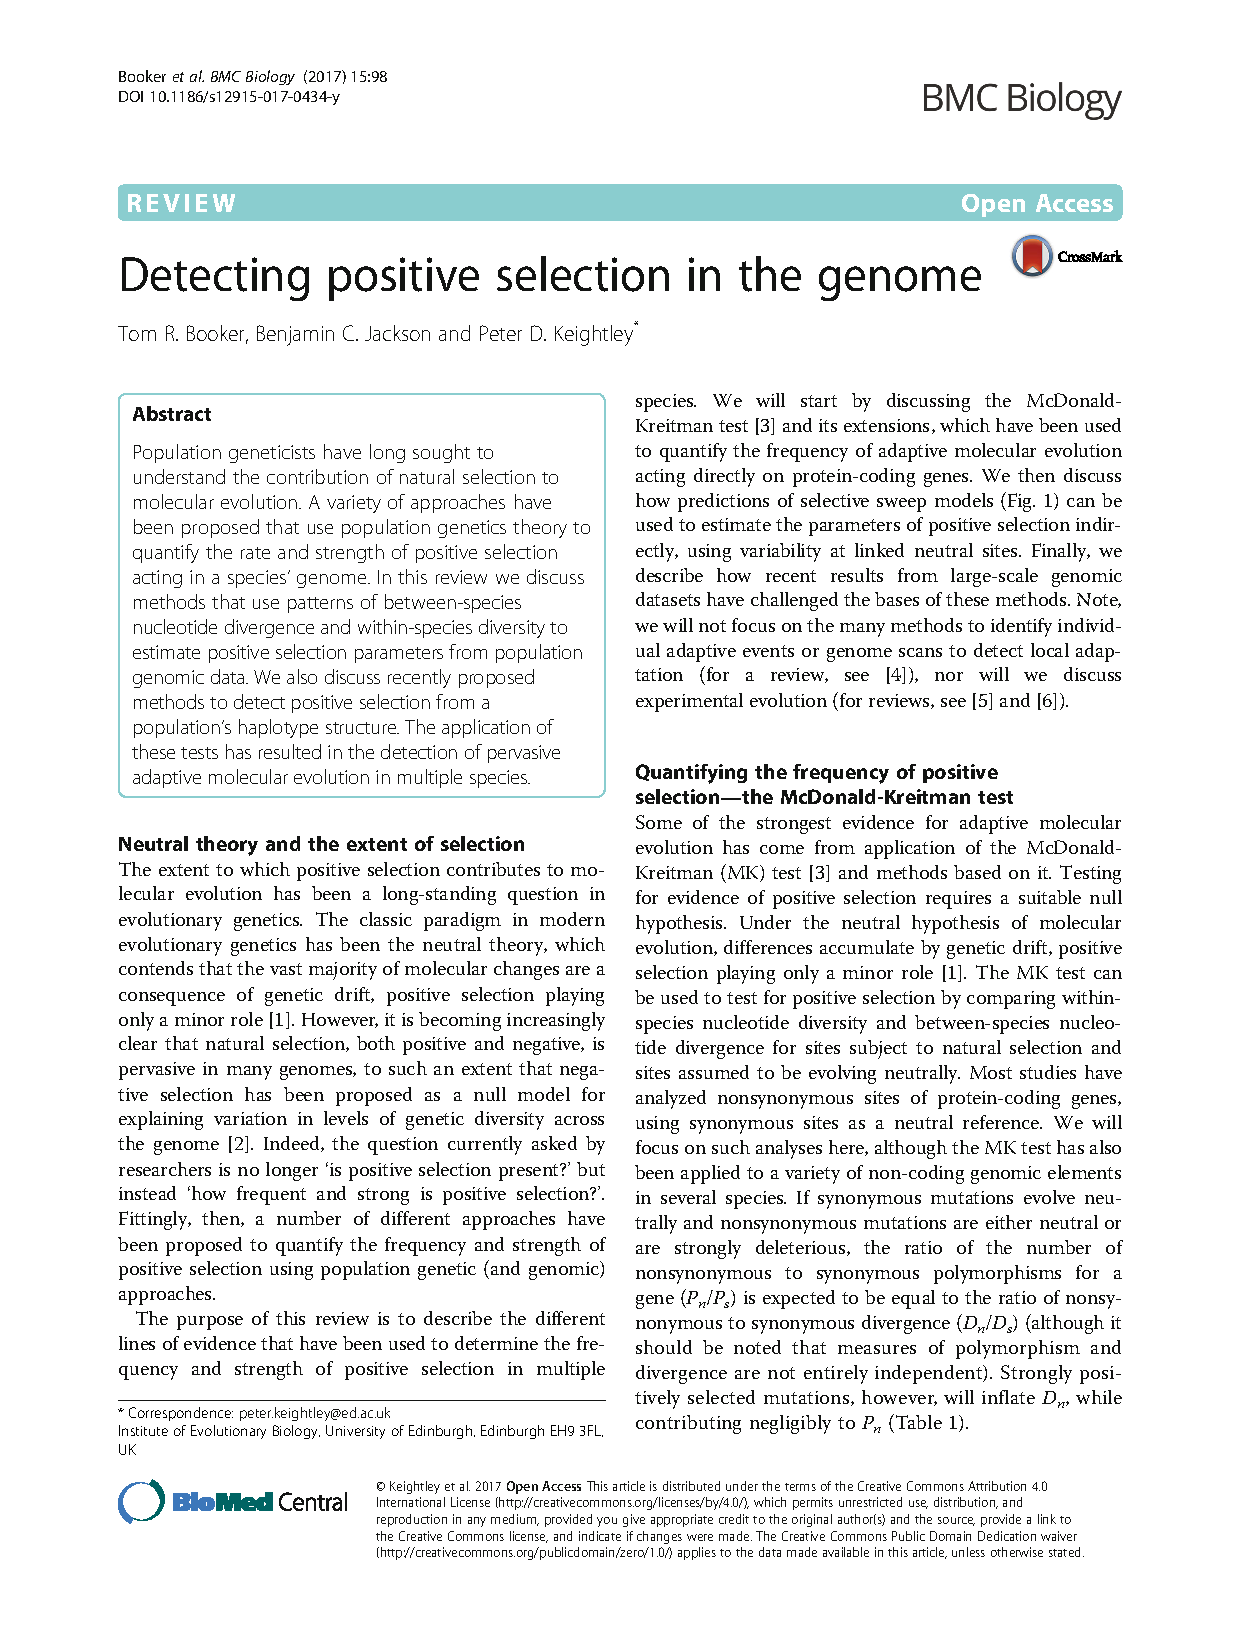
\includepdf[pages=-, scale = 0.8 , pagecommand={\pagestyle{fancy}}]{/Users/s0784966/Dropbox/Thesis/chapter1Appendix/Booker_et_al_2017_REVIEW.pdf}

		\chapter{Recombination in wild mice}

		
\section{Supplementary Material}
Included here are the supplementary figures and tables for Chapter 2.
\linespread{1}
\begin{sidewaystable}
\caption[Summary of recombination rates per chromosomes]{Summary of sex-averaged recombination rates \emph{M. m castaneus} compared with the rates from Brunschwig et al. (2012) and Cox et al. (2009). Rates for the castaneus and Brunschwig maps are presented in terms of $4N_{e}r/bp$. Estimates of $N_e$ were obtained by assuming the recombination rates from Cox et al. (2009).}
 \begin{tabular}{c c c c c c c c c } 
  \hline
& & &  & & \multicolumn{3}{c}{Switch Errors} &  \\
Filter Set & HWE & Min DP & Max DP & Min GQ & H40 & H46 & H62 & \\ \hline
1 & - & - & - & - & 5,148/409,486 & 4,819/407,422 & 5,020/394,778 & 0.0124 \\
2 & <0.0002 & 10 & - & 15 & 1,690/338,592 & 1,451/334,111 & 1,452/324,199 & 0.0046 \\
3 & <0.0002 & 10 & 100 & 5 & 2,460 /341,744 & 2066 /339,508 & 2536 /328,998 & 0.0070 \\
4 & <0.0002 & - & - & 40 & 523 /288,471 & 444 /286,636 & 550 /281,266 & 0.0018 \\
 \hline
\end{tabular}    
 \label{tab:C2ST1}
\end{sidewaystable}

	
\begin{table}[h!]
\centering
\caption[Parameters of the best-fitting demographic model estimated from the analysis of 4-fold and CNE-flanking sites]{Parameters of the best-fitting demographic model estimated from the analysis of 4-fold and CNE-flanking sites. }
 \begin{tabular}{c c c c c } 

\toprule
	&4-fold	&CNE-flank \\ \hline
N2/N1&	0.40&	0.07 \\
t2/N1&	0.44&	0.17 \\
N3/N1&	0.40&	1.00 \\
t3/N1&	1.10&	0.63 \\
\bottomrule

\end{tabular}
\label{tab:CS2}
\end{table}
\begin{table}[h!]
\centering
\caption[Parameters of the 3-epoch demographic model at different sample sizes]{Parameters of the 3-epoch demographic model at different sample sizes. Down sampled datasets were generated by randomly selecting alleles, with respect to frequency, from the full dataset of 10 individuals.}
 \begin{tabular}{c c c c c } 

\toprule
\multirow{2}{*}{Parameter} & \multicolumn{3}{c}{Number of alleles sampled} \\ 
	&	$n = 10$ & 	$n = 16$ & 	$n = 20$ \\ \hline
N2/N1 &	0.030 &	0.030 &	0.060 \\
t2/N1 &	0.204 &	0.140 &	0.181 \\
N3/N1 &	0.120 &	0.200 &	0.800 \\
t3/N1 &	0.080 &	0.220 &	0.461 \\
\bottomrule

\end{tabular}
\label{tab:CS3}
\end{table}


\begin{table}
\caption{The overlap between the hotspots we identified in M. m. castaneus and the locations of DSB hotspots in wild-derived strains obtained by Smagulova et al. (2016). The corrected overlap is the number of overlapping hotspots, above the null expectation, over the total.}
\begin{tabular} {c c c c c c c} \\ [ 0.5ex ] \hline

\makecell{Strain\\ID} & Sub-species & \makecell{\# DSB \\ Hotspots} & \makecell{\# \\ Overlaps} & \makecell{\% Overlap \\ Uncorrected} & \makecell{Null \\Expectation} & \makecell{\% Overlap \\ Corrected}\\ \hline
13R & \emph{domesticus} & 14744 & 1202 & 8.2 & 1169 & 0.2 \\
B6 & \emph{domesticus}& 19455 & 1533 & 7.9 & 1505 & 0.1 \\ 
C3H & \emph{domesticus} & 14635 & 1399 & 9.6 & 1308 & 0.6 \\
CAST & \emph{castaneus} & 15061 & 1831 & 12.2 & 1221 & 4.1 \\
MOL & \emph{molossinus} & 15718 & 1559 & 9.9 & 1351 & 1.3 \\
PWD & \emph{musculus} & 14483 & 1569 & 10.8 & 1205 & 2.5 \\ \hline


\end{tabular}
\end{table}

 
 \begin{figure}
   \centering      
   \noindent\makebox[\textwidth]{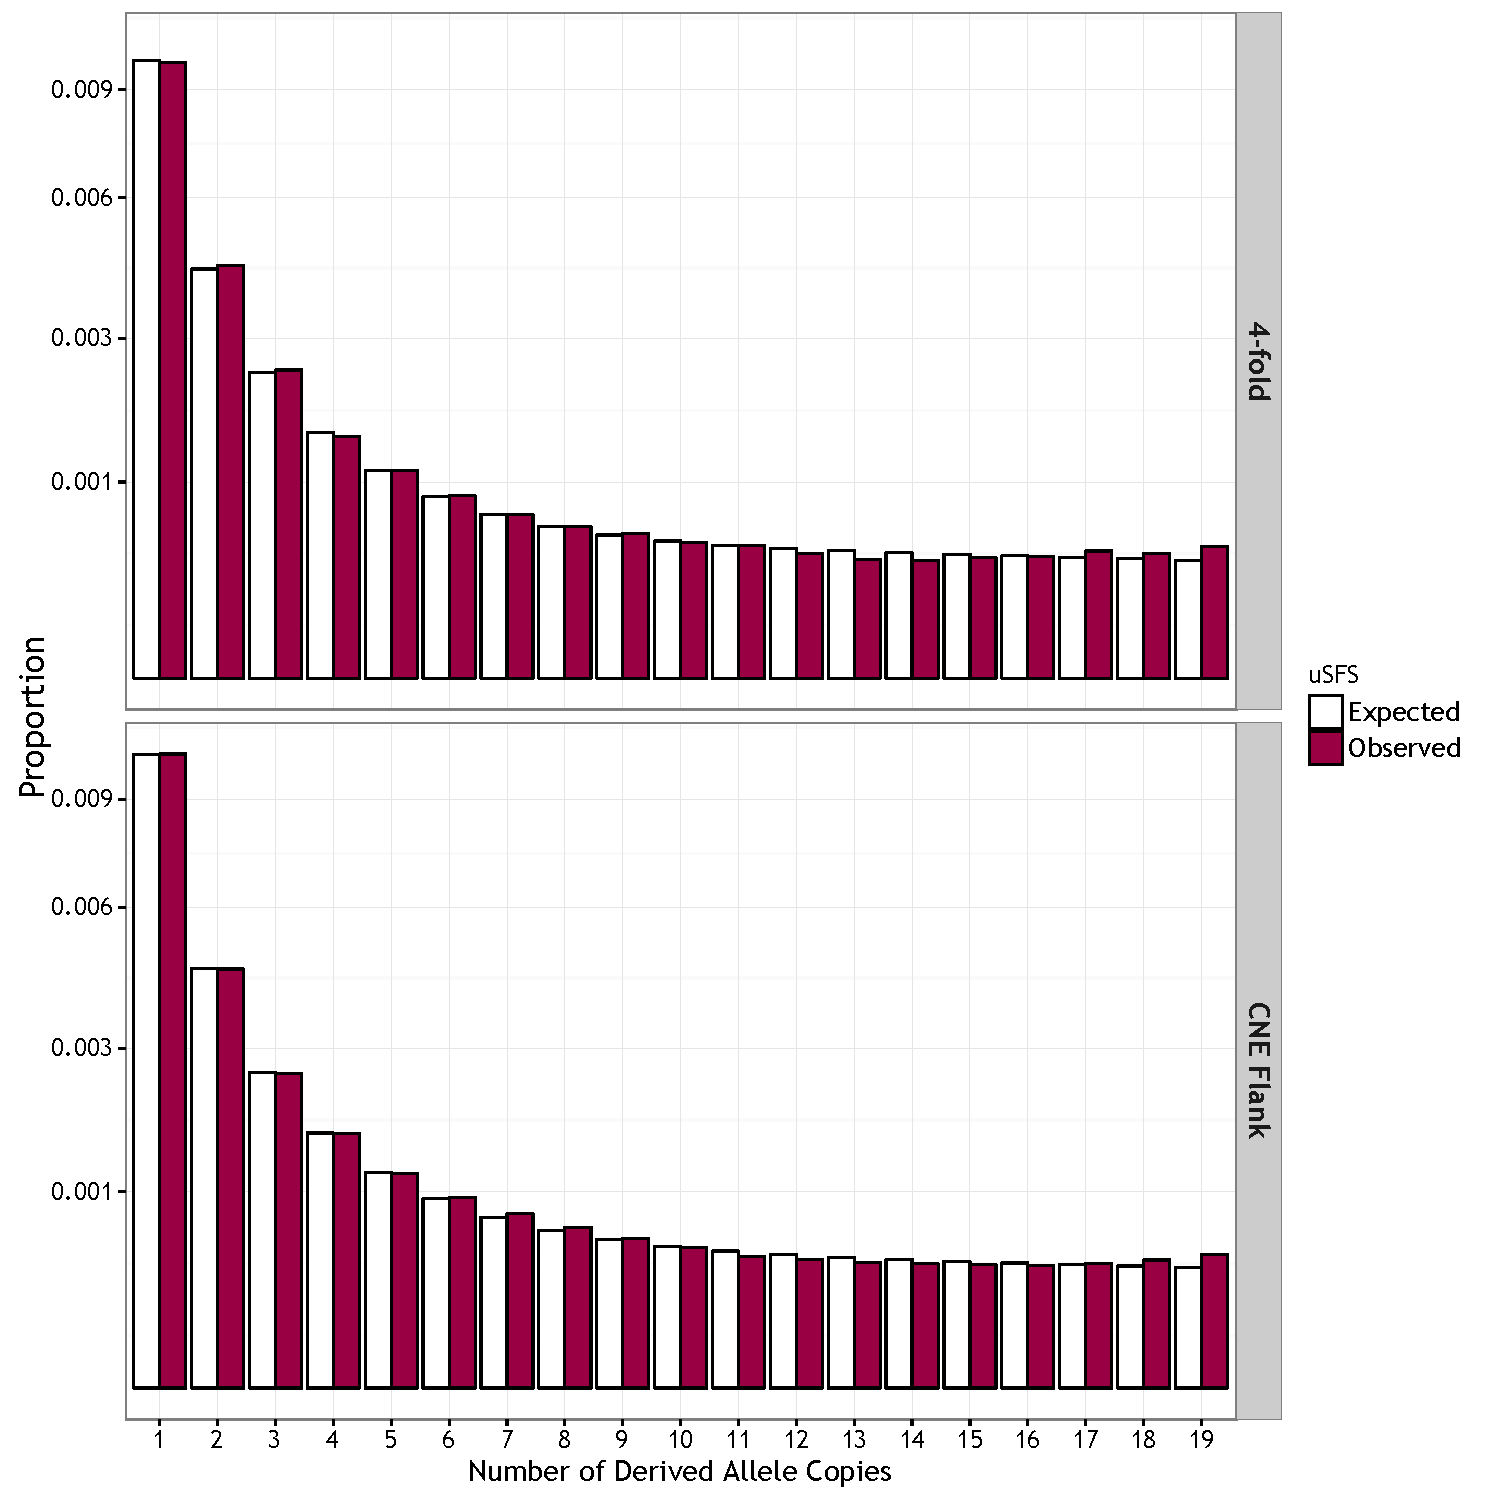
\includegraphics[width=\textwidth]{/Users/s0784966/Dropbox/Thesis/chapter2Appendix/Figures/FigureS1.pdf}}
 \caption[]{}
 \label{fig:1}
\end{figure}

 
 \begin{figure}
   \centering      
   \noindent\makebox[\textwidth]{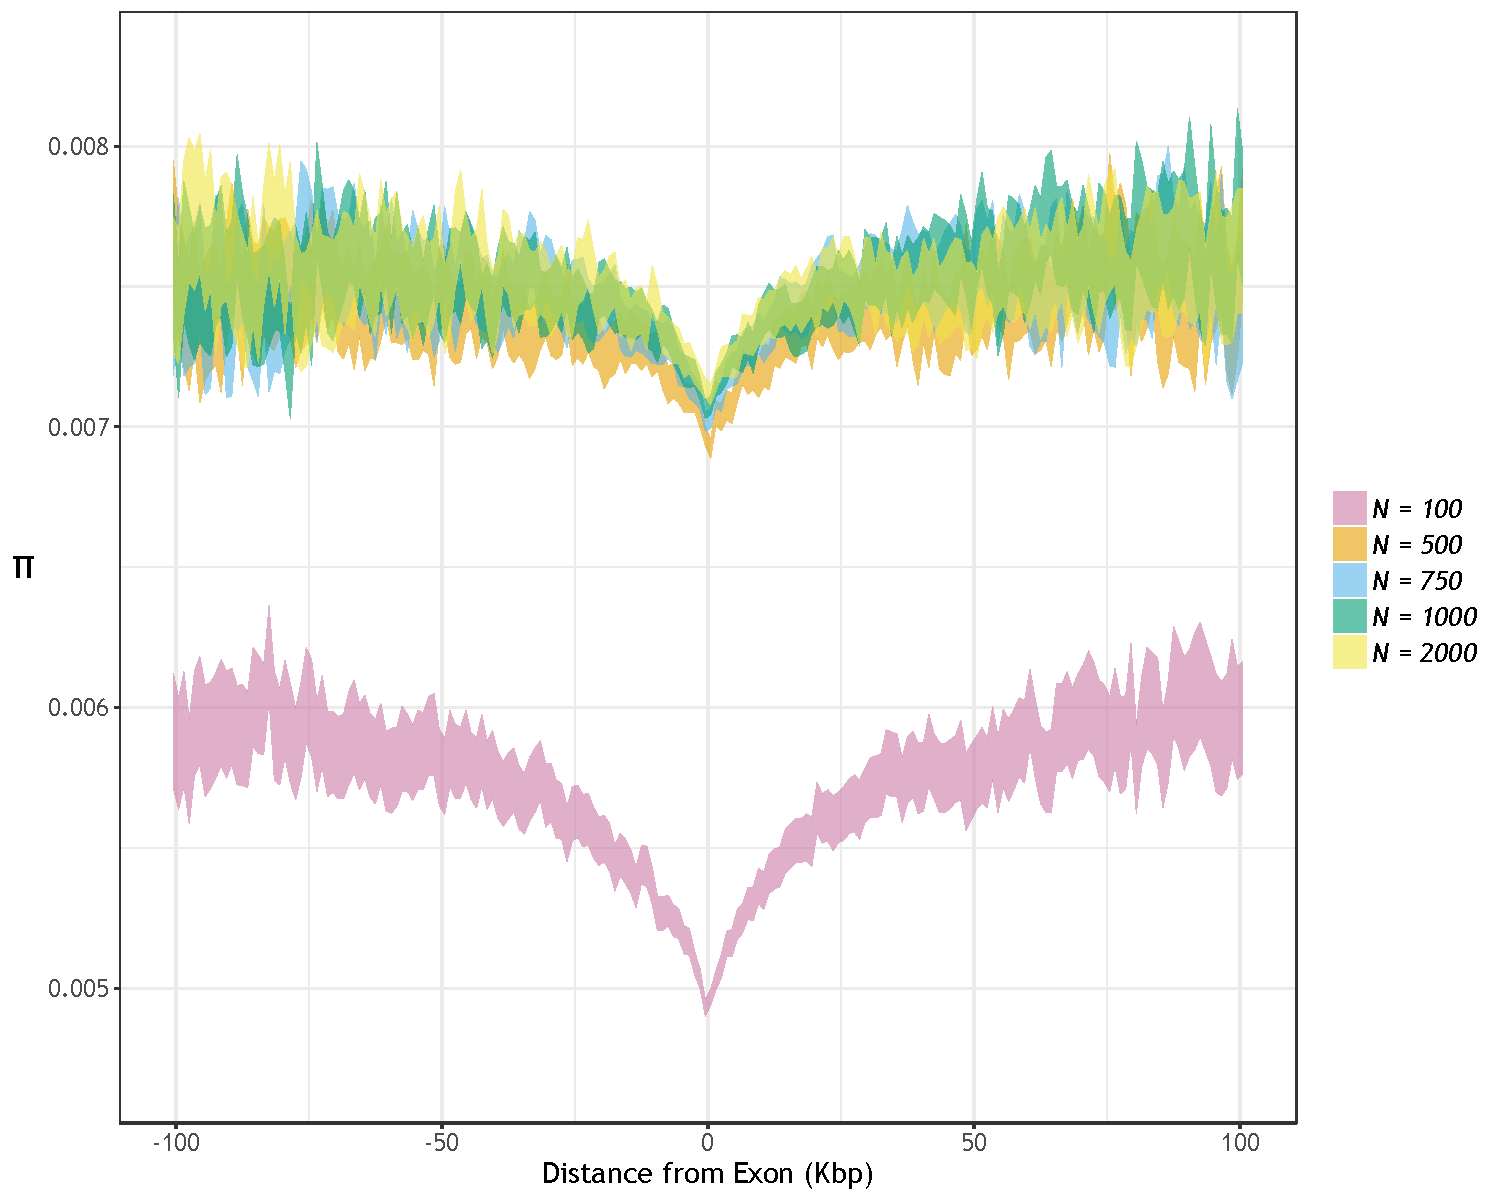
\includegraphics[width=\textwidth]{/Users/s0784966/Dropbox/Thesis/chapter2Appendix/Figures/FigureS2.pdf}}
 \caption[The effect of switch errors on recombination rate inference]{The effect of switch errors on the mean recombination rate inferred using LDhelmet with a block penalty of 100. Each black point represents results for a window of 4000 SNPs, with 200 SNPs overlapping between adjacent windows, using sequences simulated in SLiM for a constant value of $\rho/bp$. Red points are mean values. Switch errors were randomly incorporated at heterozygous SNPs with probability 0.0046. The dotted line shows the value when the inferred and true rates are equal}
 \label{fig:1}
\end{figure}

 
 \begin{figure}
   \centering      
   \noindent\makebox[\textwidth]{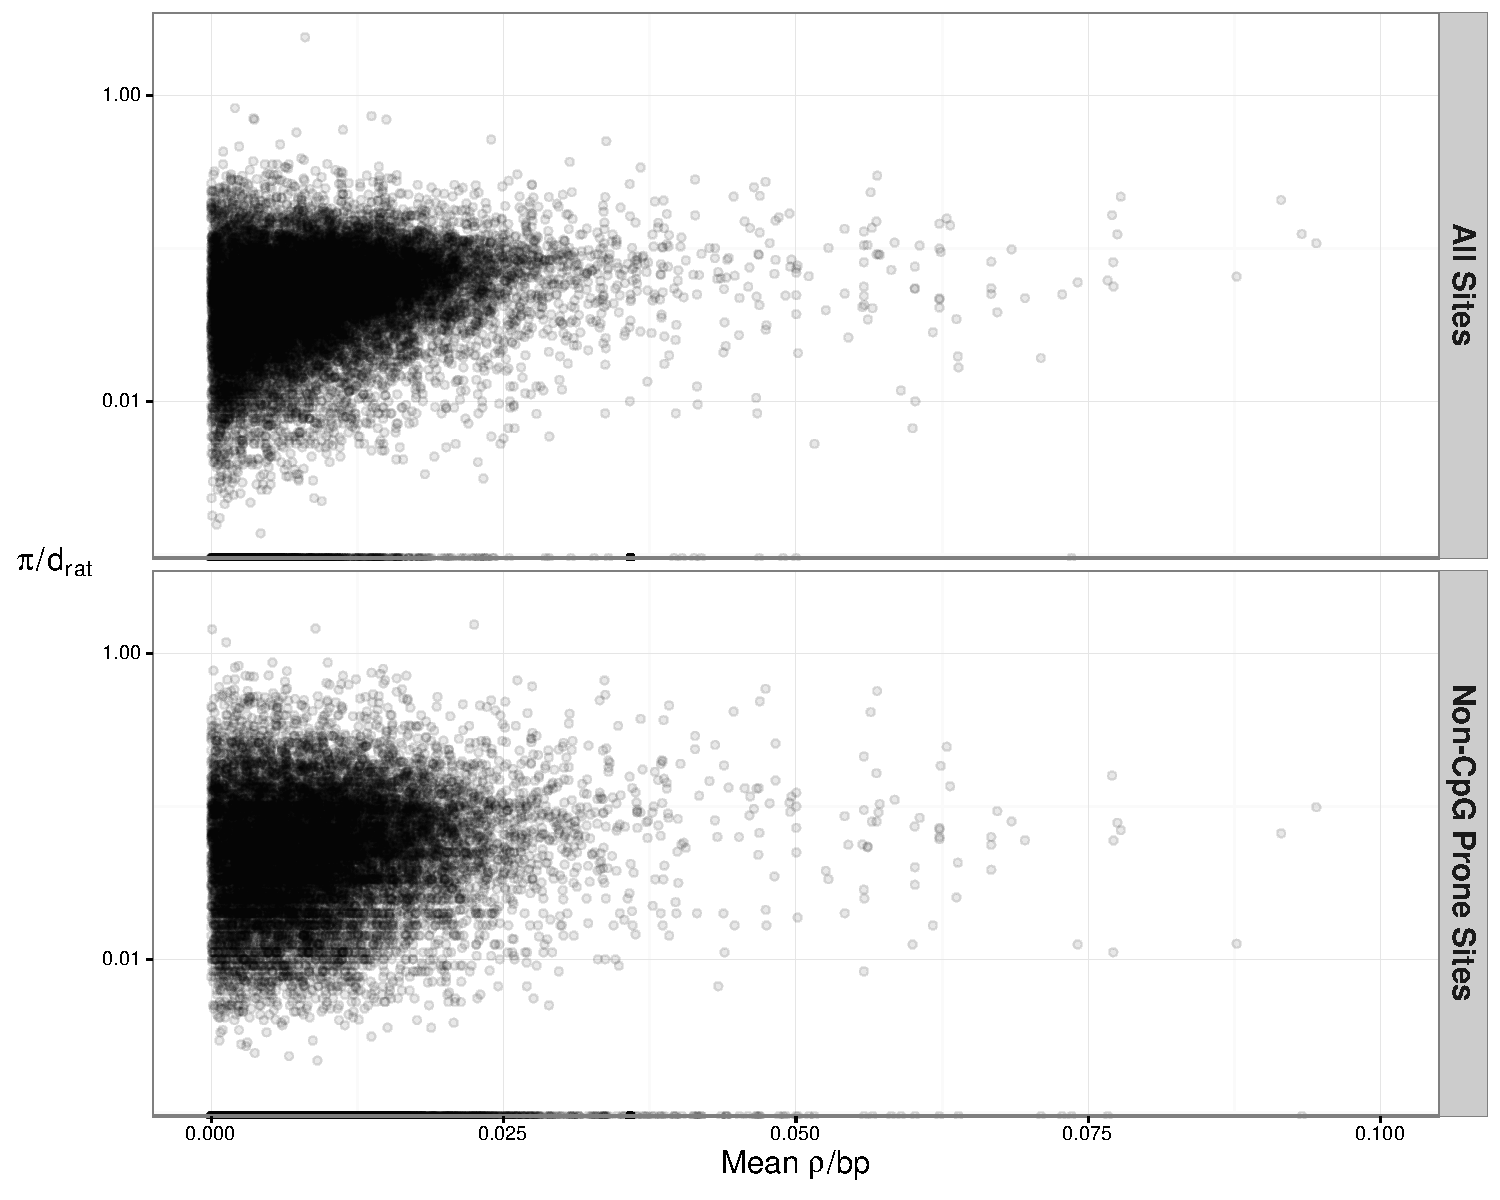
\includegraphics[width=\textwidth]{/Users/s0784966/Dropbox/Thesis/chapter2Appendix/Figures/FigureS3.pdf}}
 \caption[The effect of switch errors on recombination rate inference]{The effect of switch errors on the mean recombination rate inferred using LDhelmet with a block penalty of 100. Each black point represents results for a window of 4000 SNPs, with 200 SNPs overlapping between adjacent windows, using sequences simulated in SLiM for a constant value of $\rho/bp$. Red points are mean values. Switch errors were randomly incorporated at heterozygous SNPs with probability 0.0046. The dotted line shows the value when the inferred and true rates are equal}
 \label{fig:1}
\end{figure}

\linespread{2}
\pagebreak
\section{Booker \emph{et al.} 2017 - Genetics}
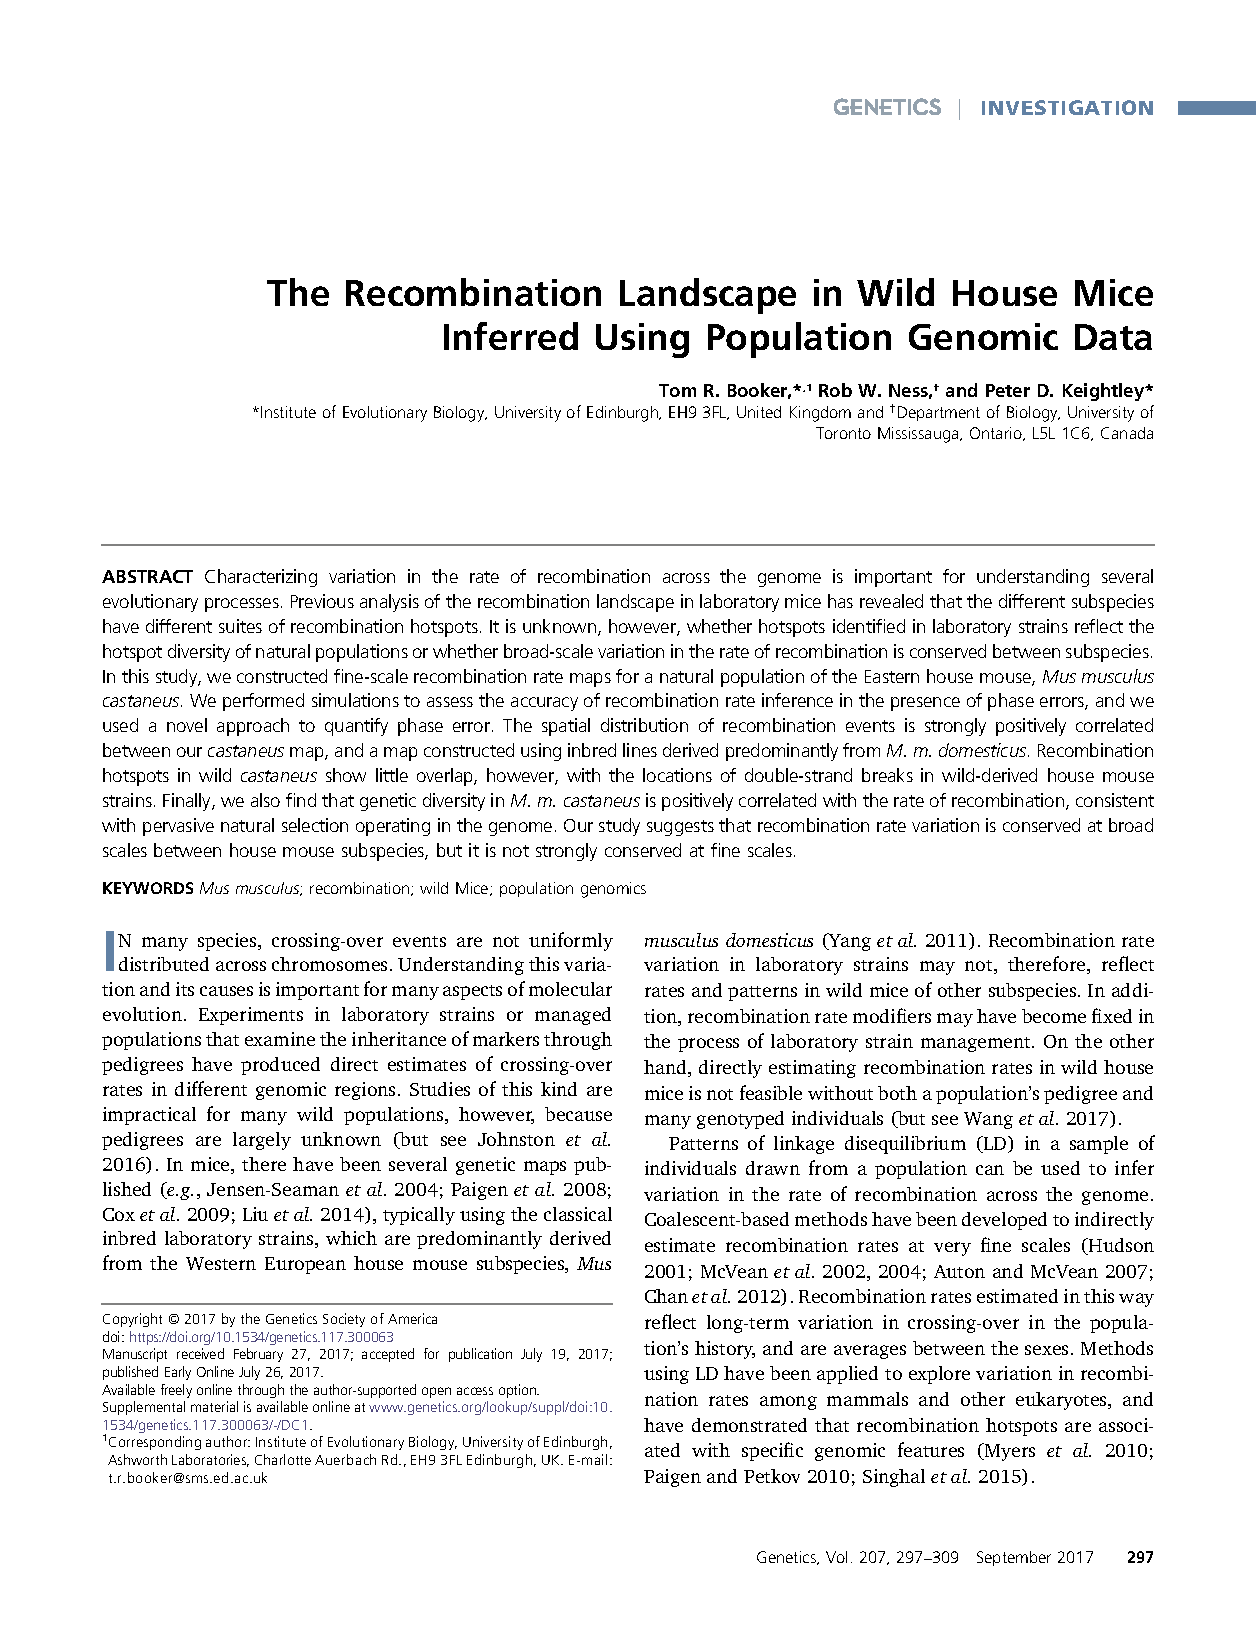
\includepdf[pages=-, scale = 0.8 , pagecommand={\pagestyle{fancy}}]{/Users/s0784966/Dropbox/Thesis/chapter2Appendix/Booker_et_al2017_Genetics.pdf}

		\chapter{Selection at linked sites in wild mice}

		\input{\dir/chapter3Appendix/chapter3appendix.tex}

		\chapter{Estimating sweep parameters}

		\input{\dir/chapter4Appendix/chapter4appendix.tex}

	\end{appendices}


\end{document}